In the following scatter plots, data points coloured black are indicated as noise. Data points with other colours highlight clusters.

\subsubsection{1h aggregated data files}

\begin{figure}[H]
	\centering
	\begin{subfigure}{.5\textwidth}
    \centering
    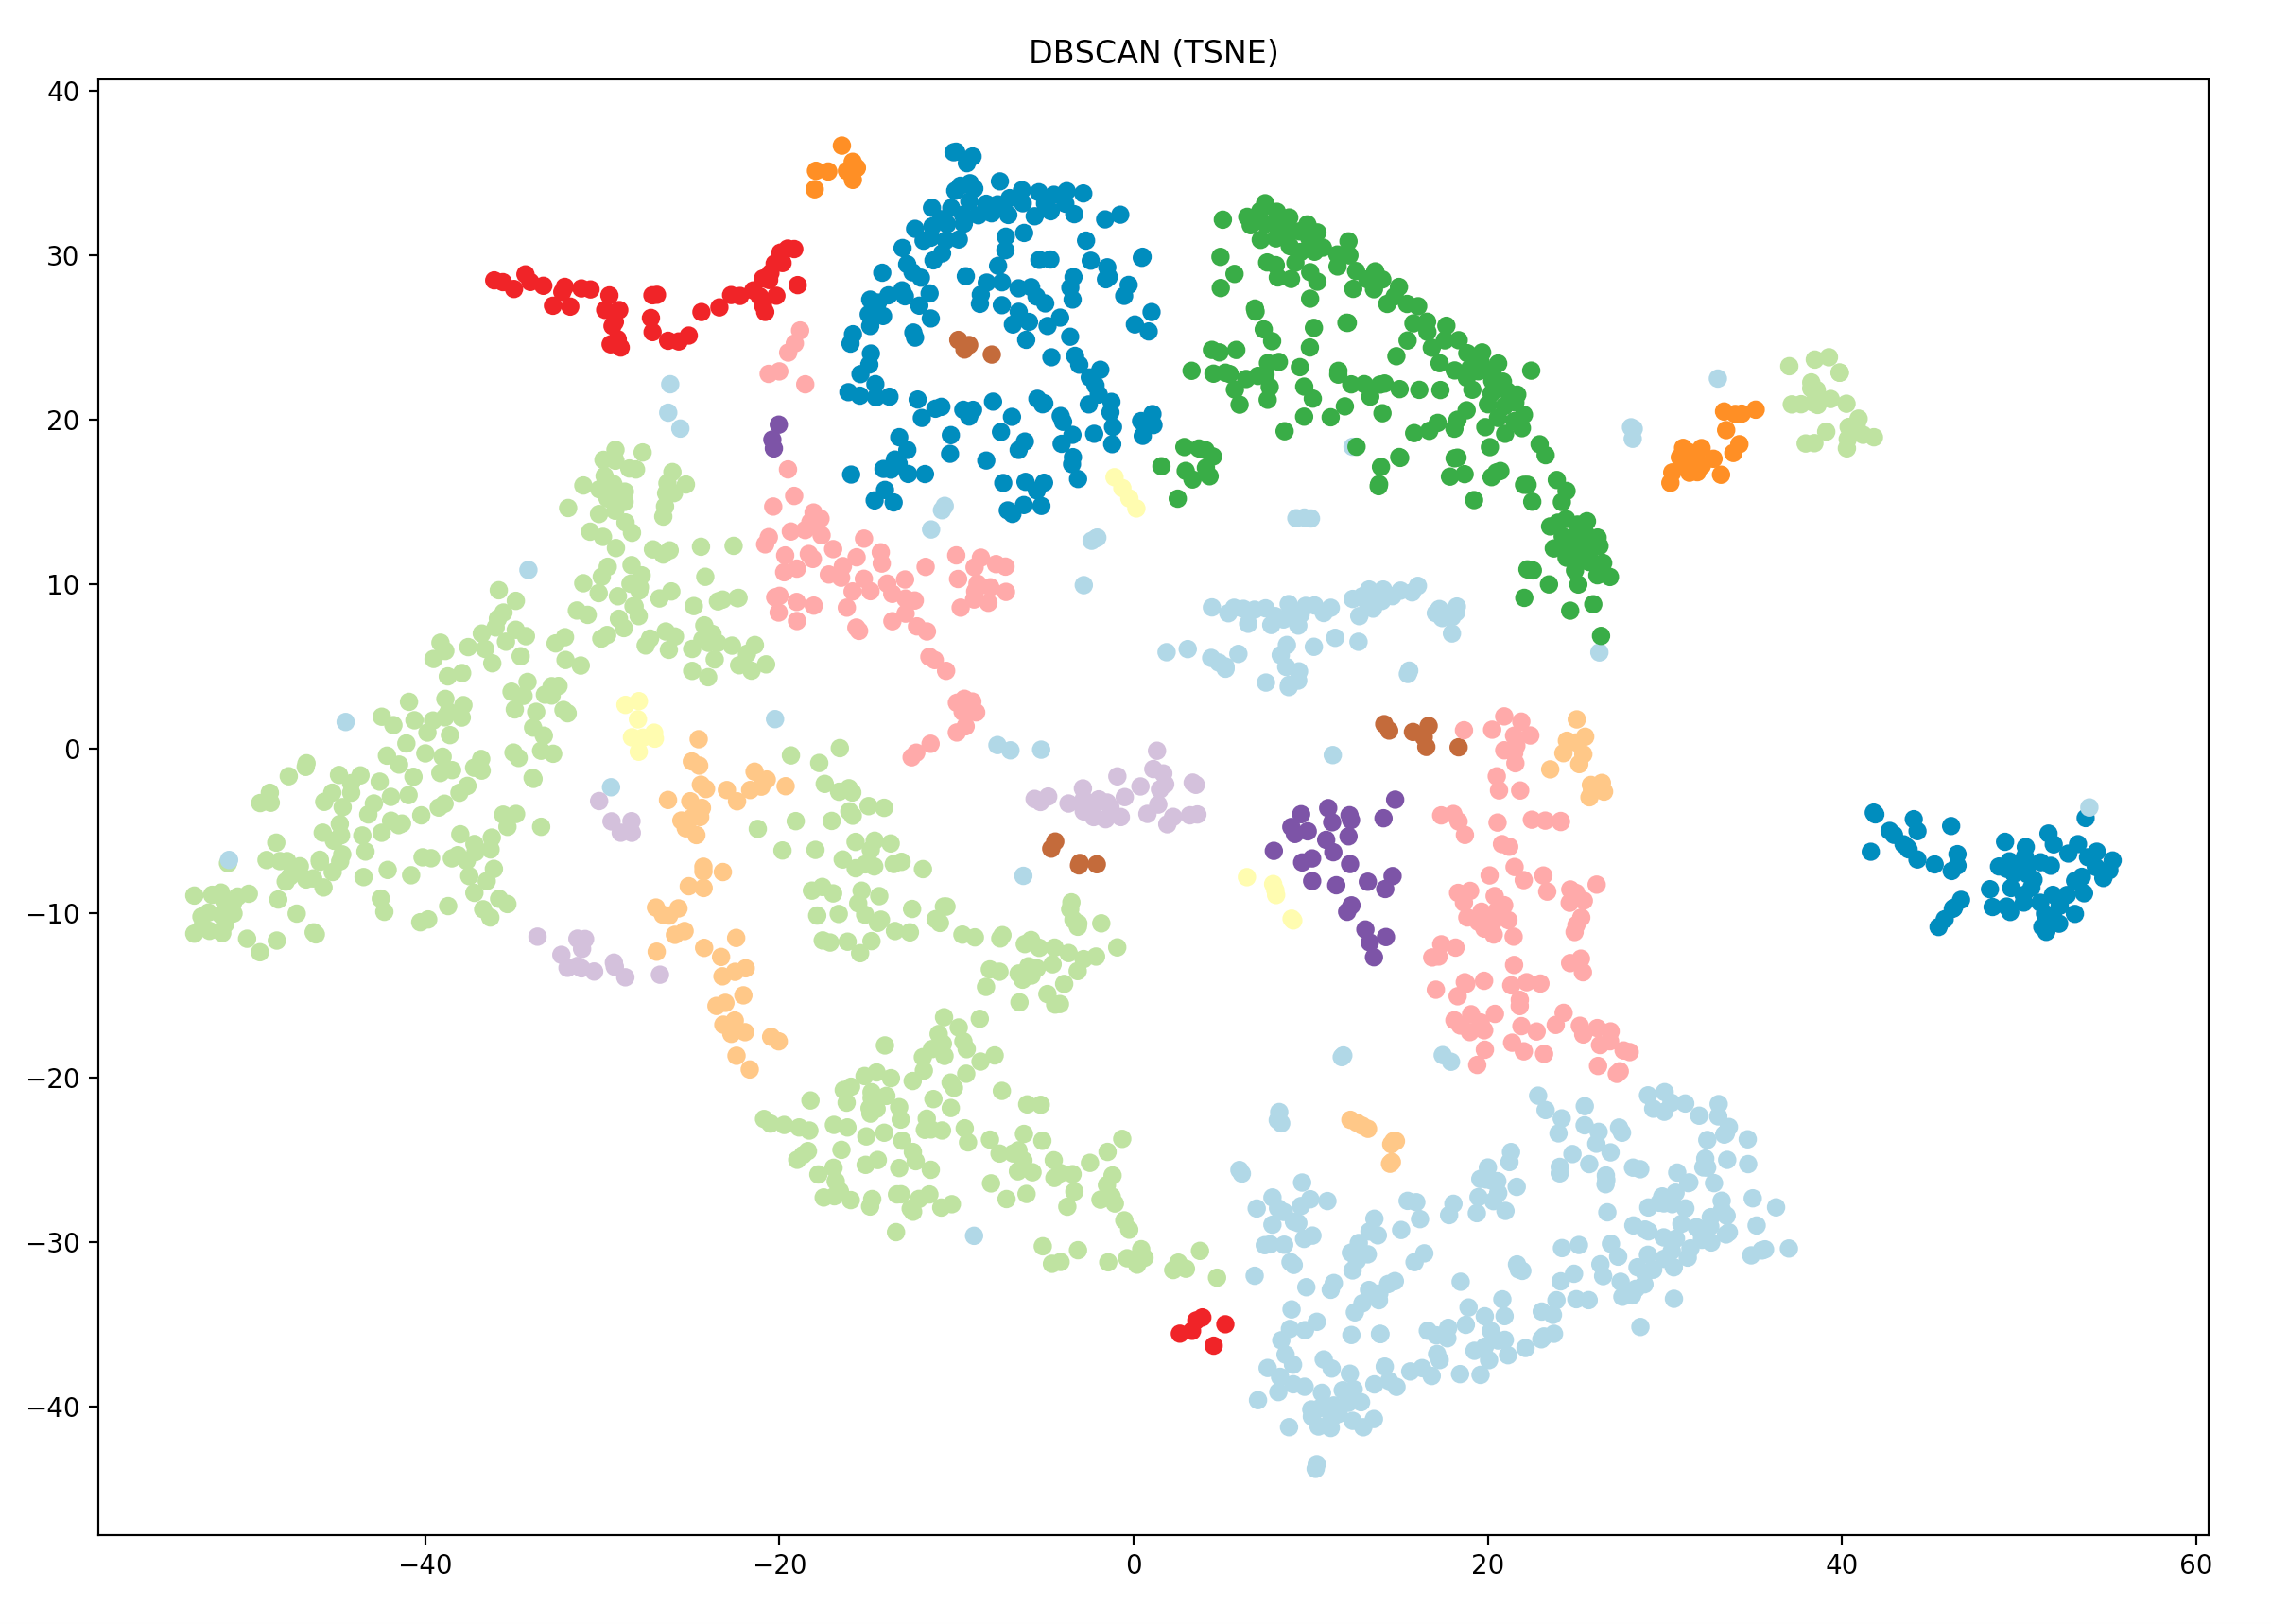
\includegraphics[width=0.9\textwidth]{./images/clusteringResults/1h-1-DBSCAN.png}
  \end{subfigure}%
  \begin{subfigure}{.5\textwidth}
    \centering
    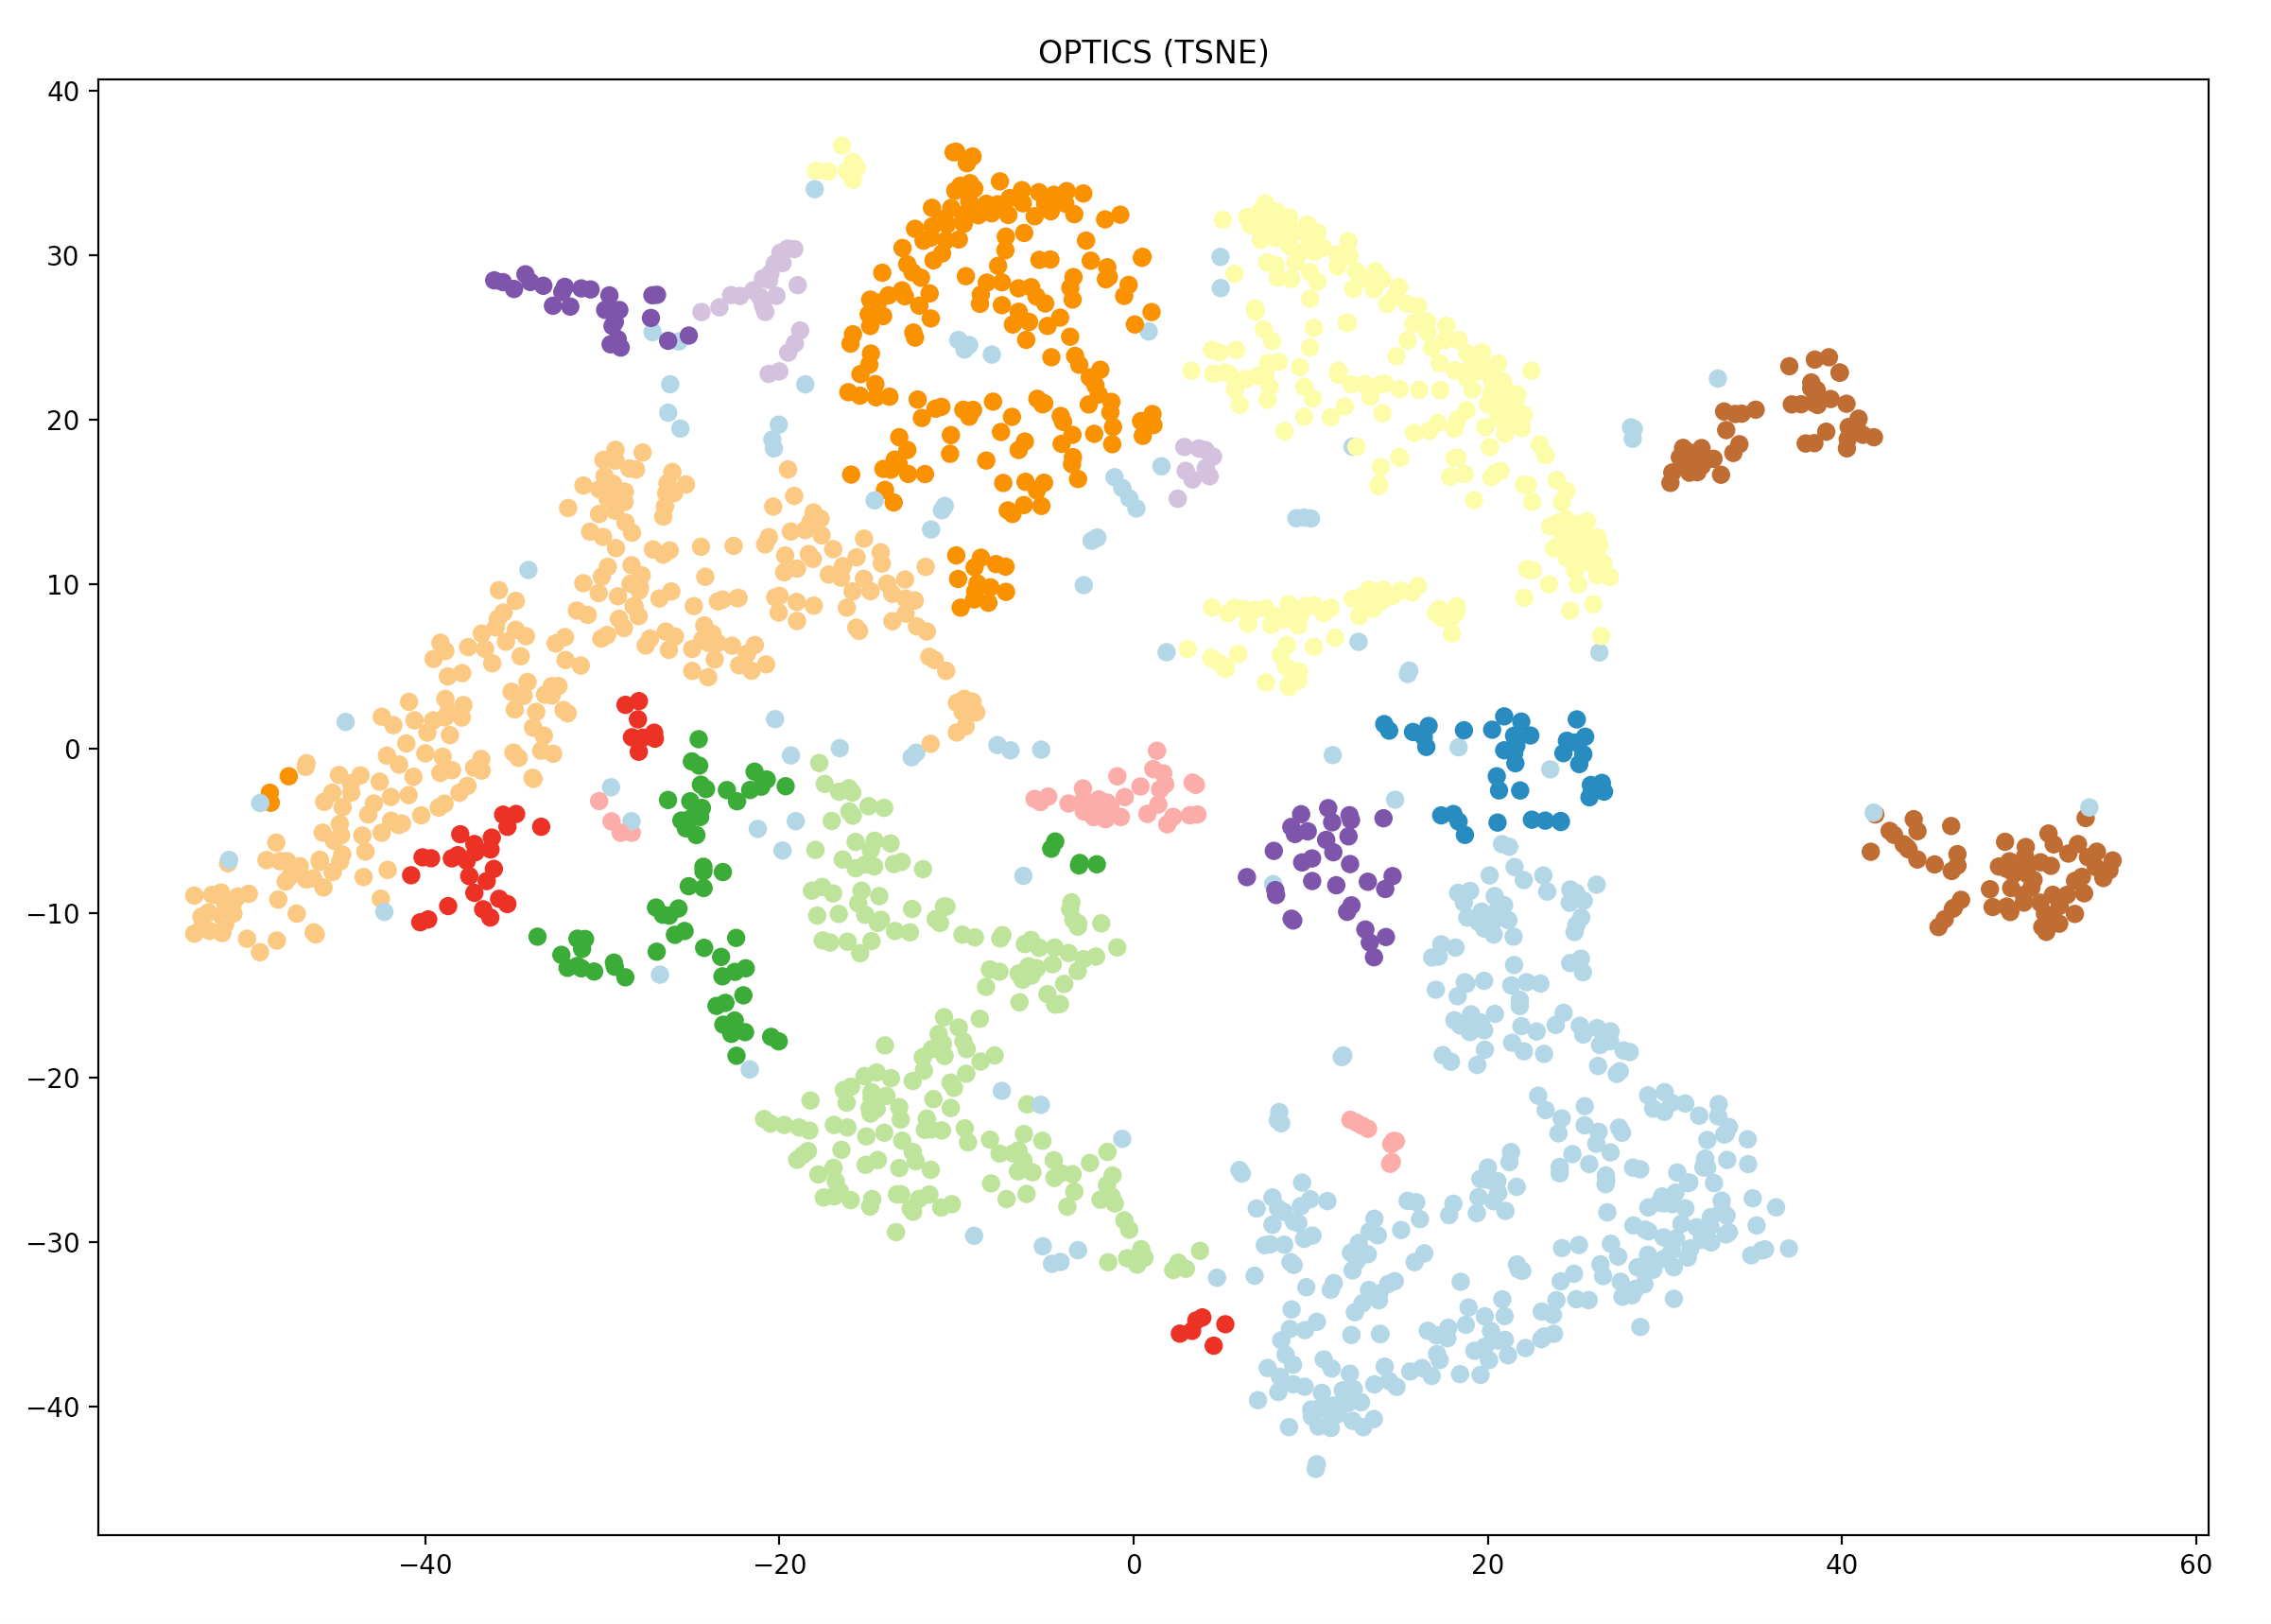
\includegraphics[width=0.9\textwidth]{./images/clusteringResults/1h-1-OPTICS.png}
	\end{subfigure}
	\caption{Comparison of the scatter plots from the DBSCAN (a) and OPTICS (b) clusterings of the 1st column, so the first \textbf{15 minutes} (1h data files: first 15 minutes).}
  \label{figure:finalClustering1h-1}
\end{figure}

\begin{figure}[H]
	\centering
	\begin{subfigure}{.5\textwidth}
    \centering
    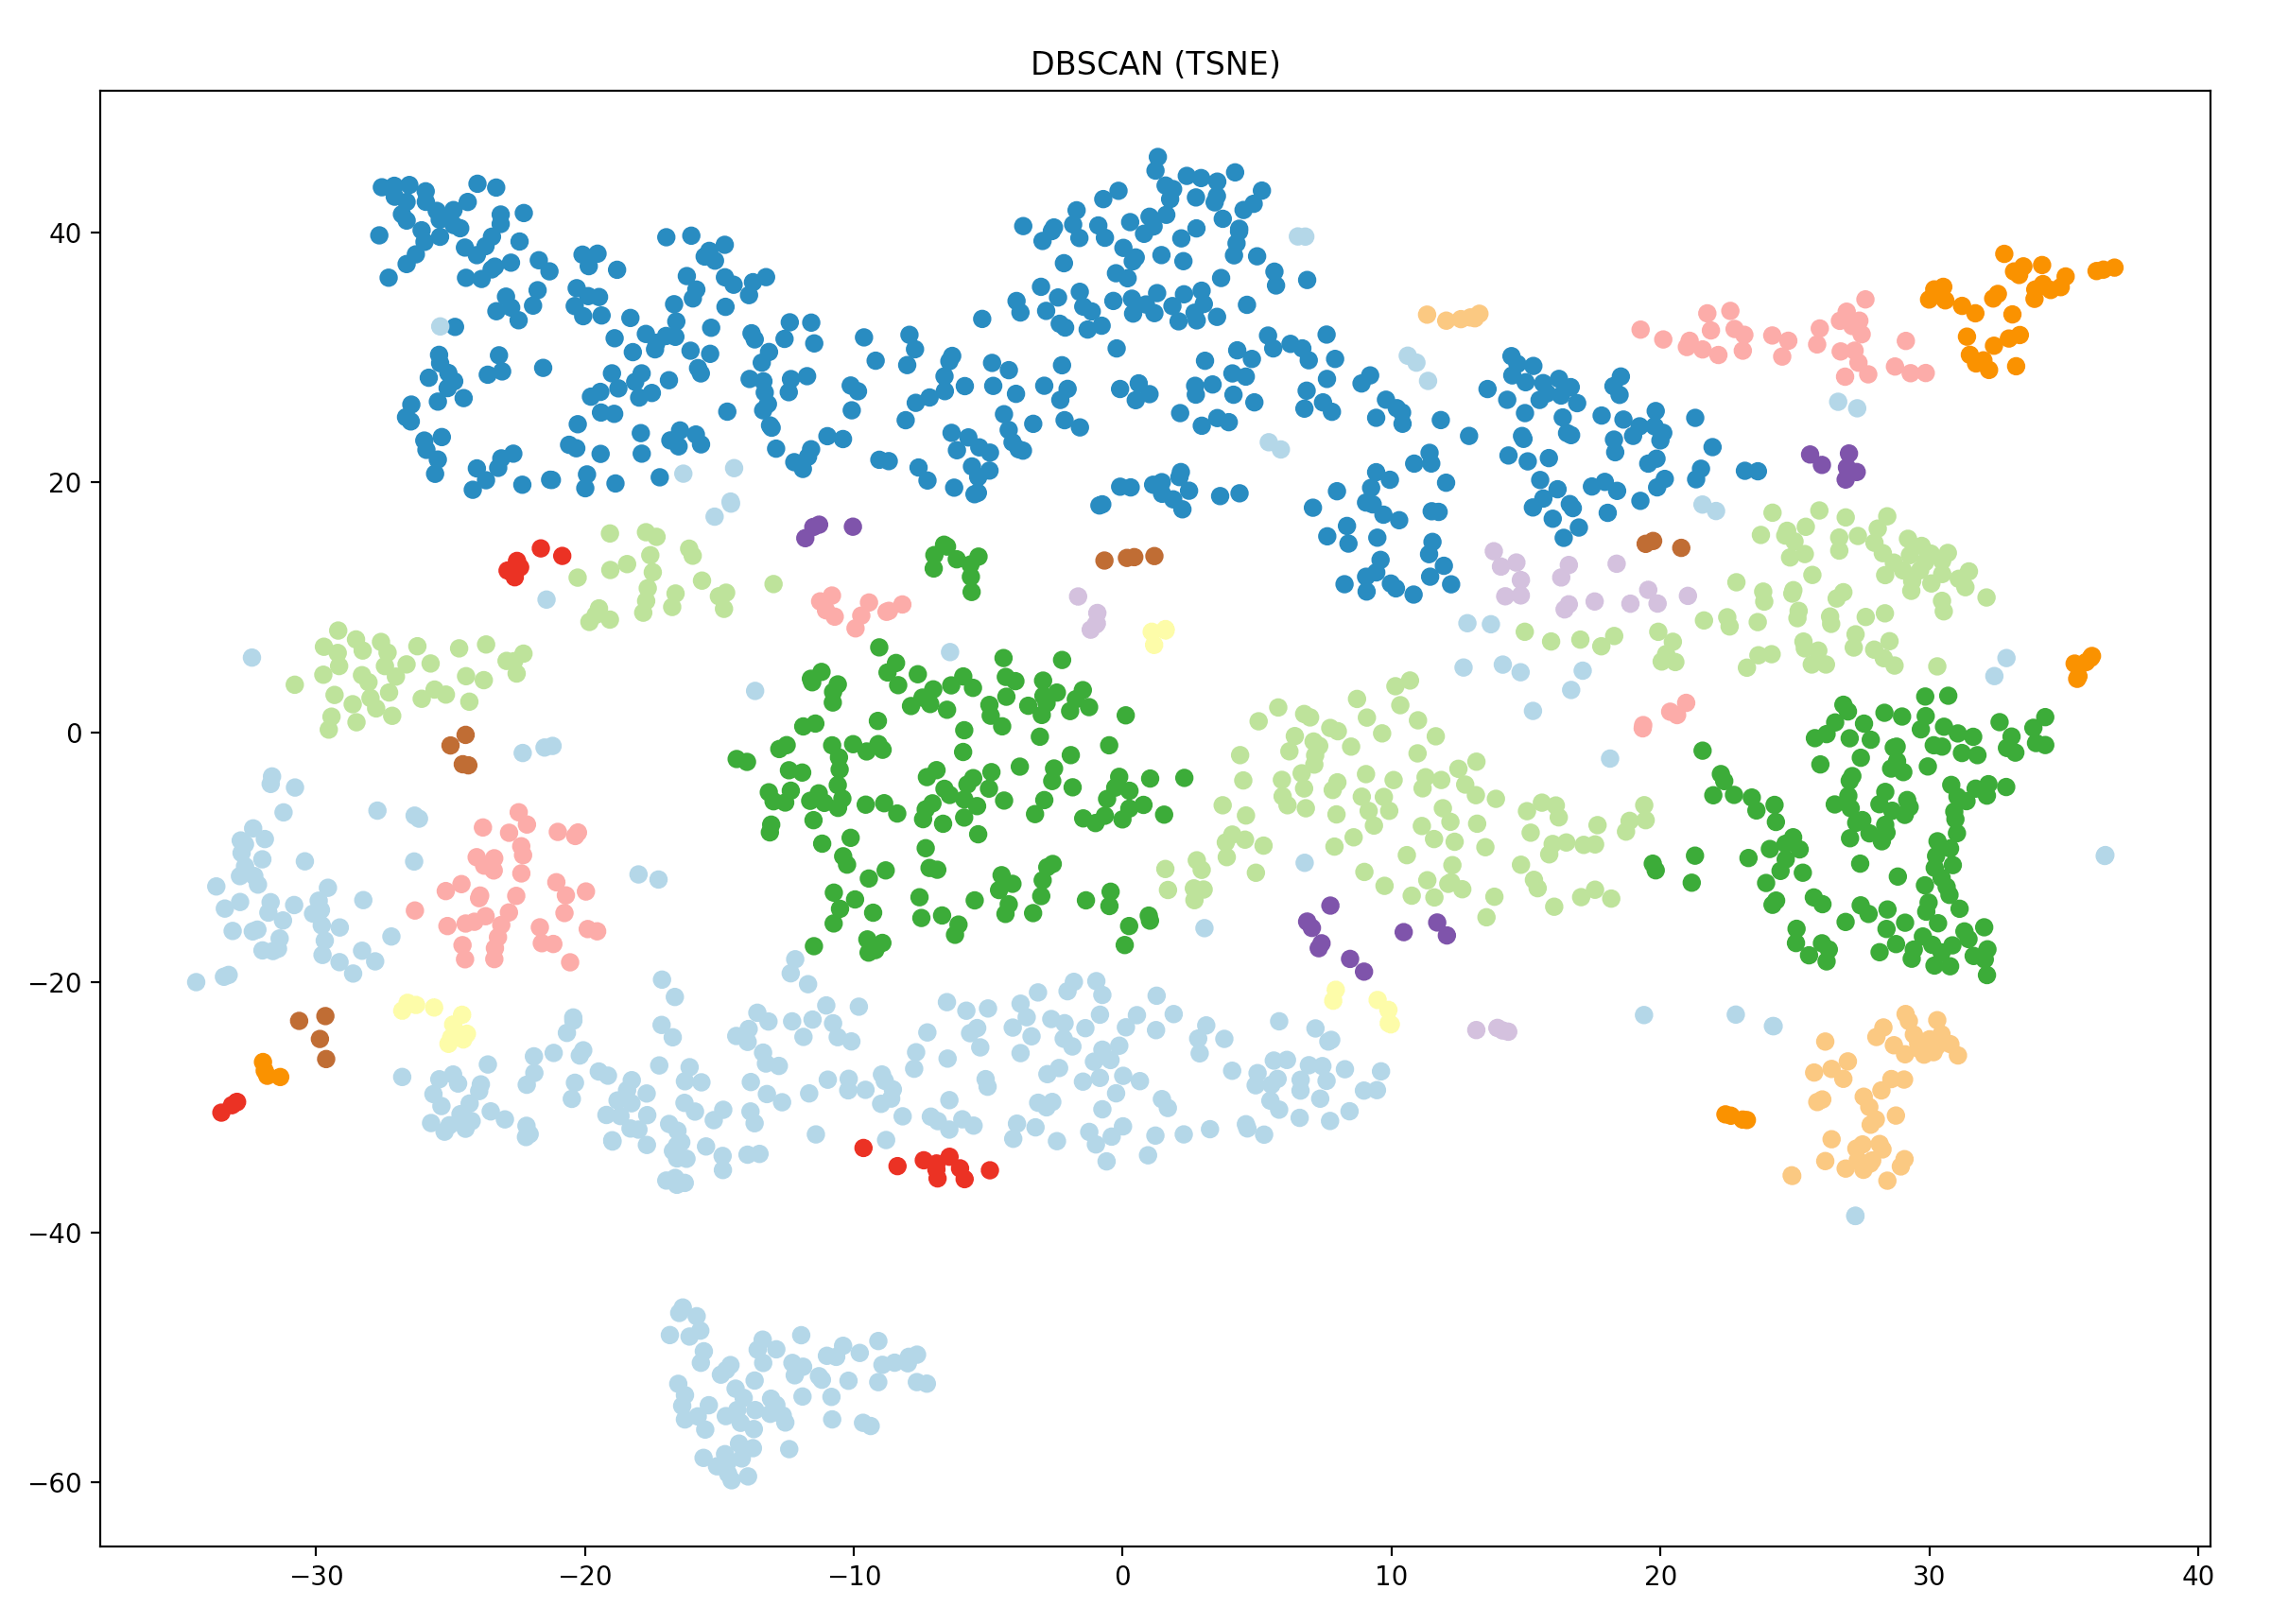
\includegraphics[width=0.9\textwidth]{./images/clusteringResults/1h-2-DBSCAN.png}
  \end{subfigure}%
  \begin{subfigure}{.5\textwidth}
    \centering
    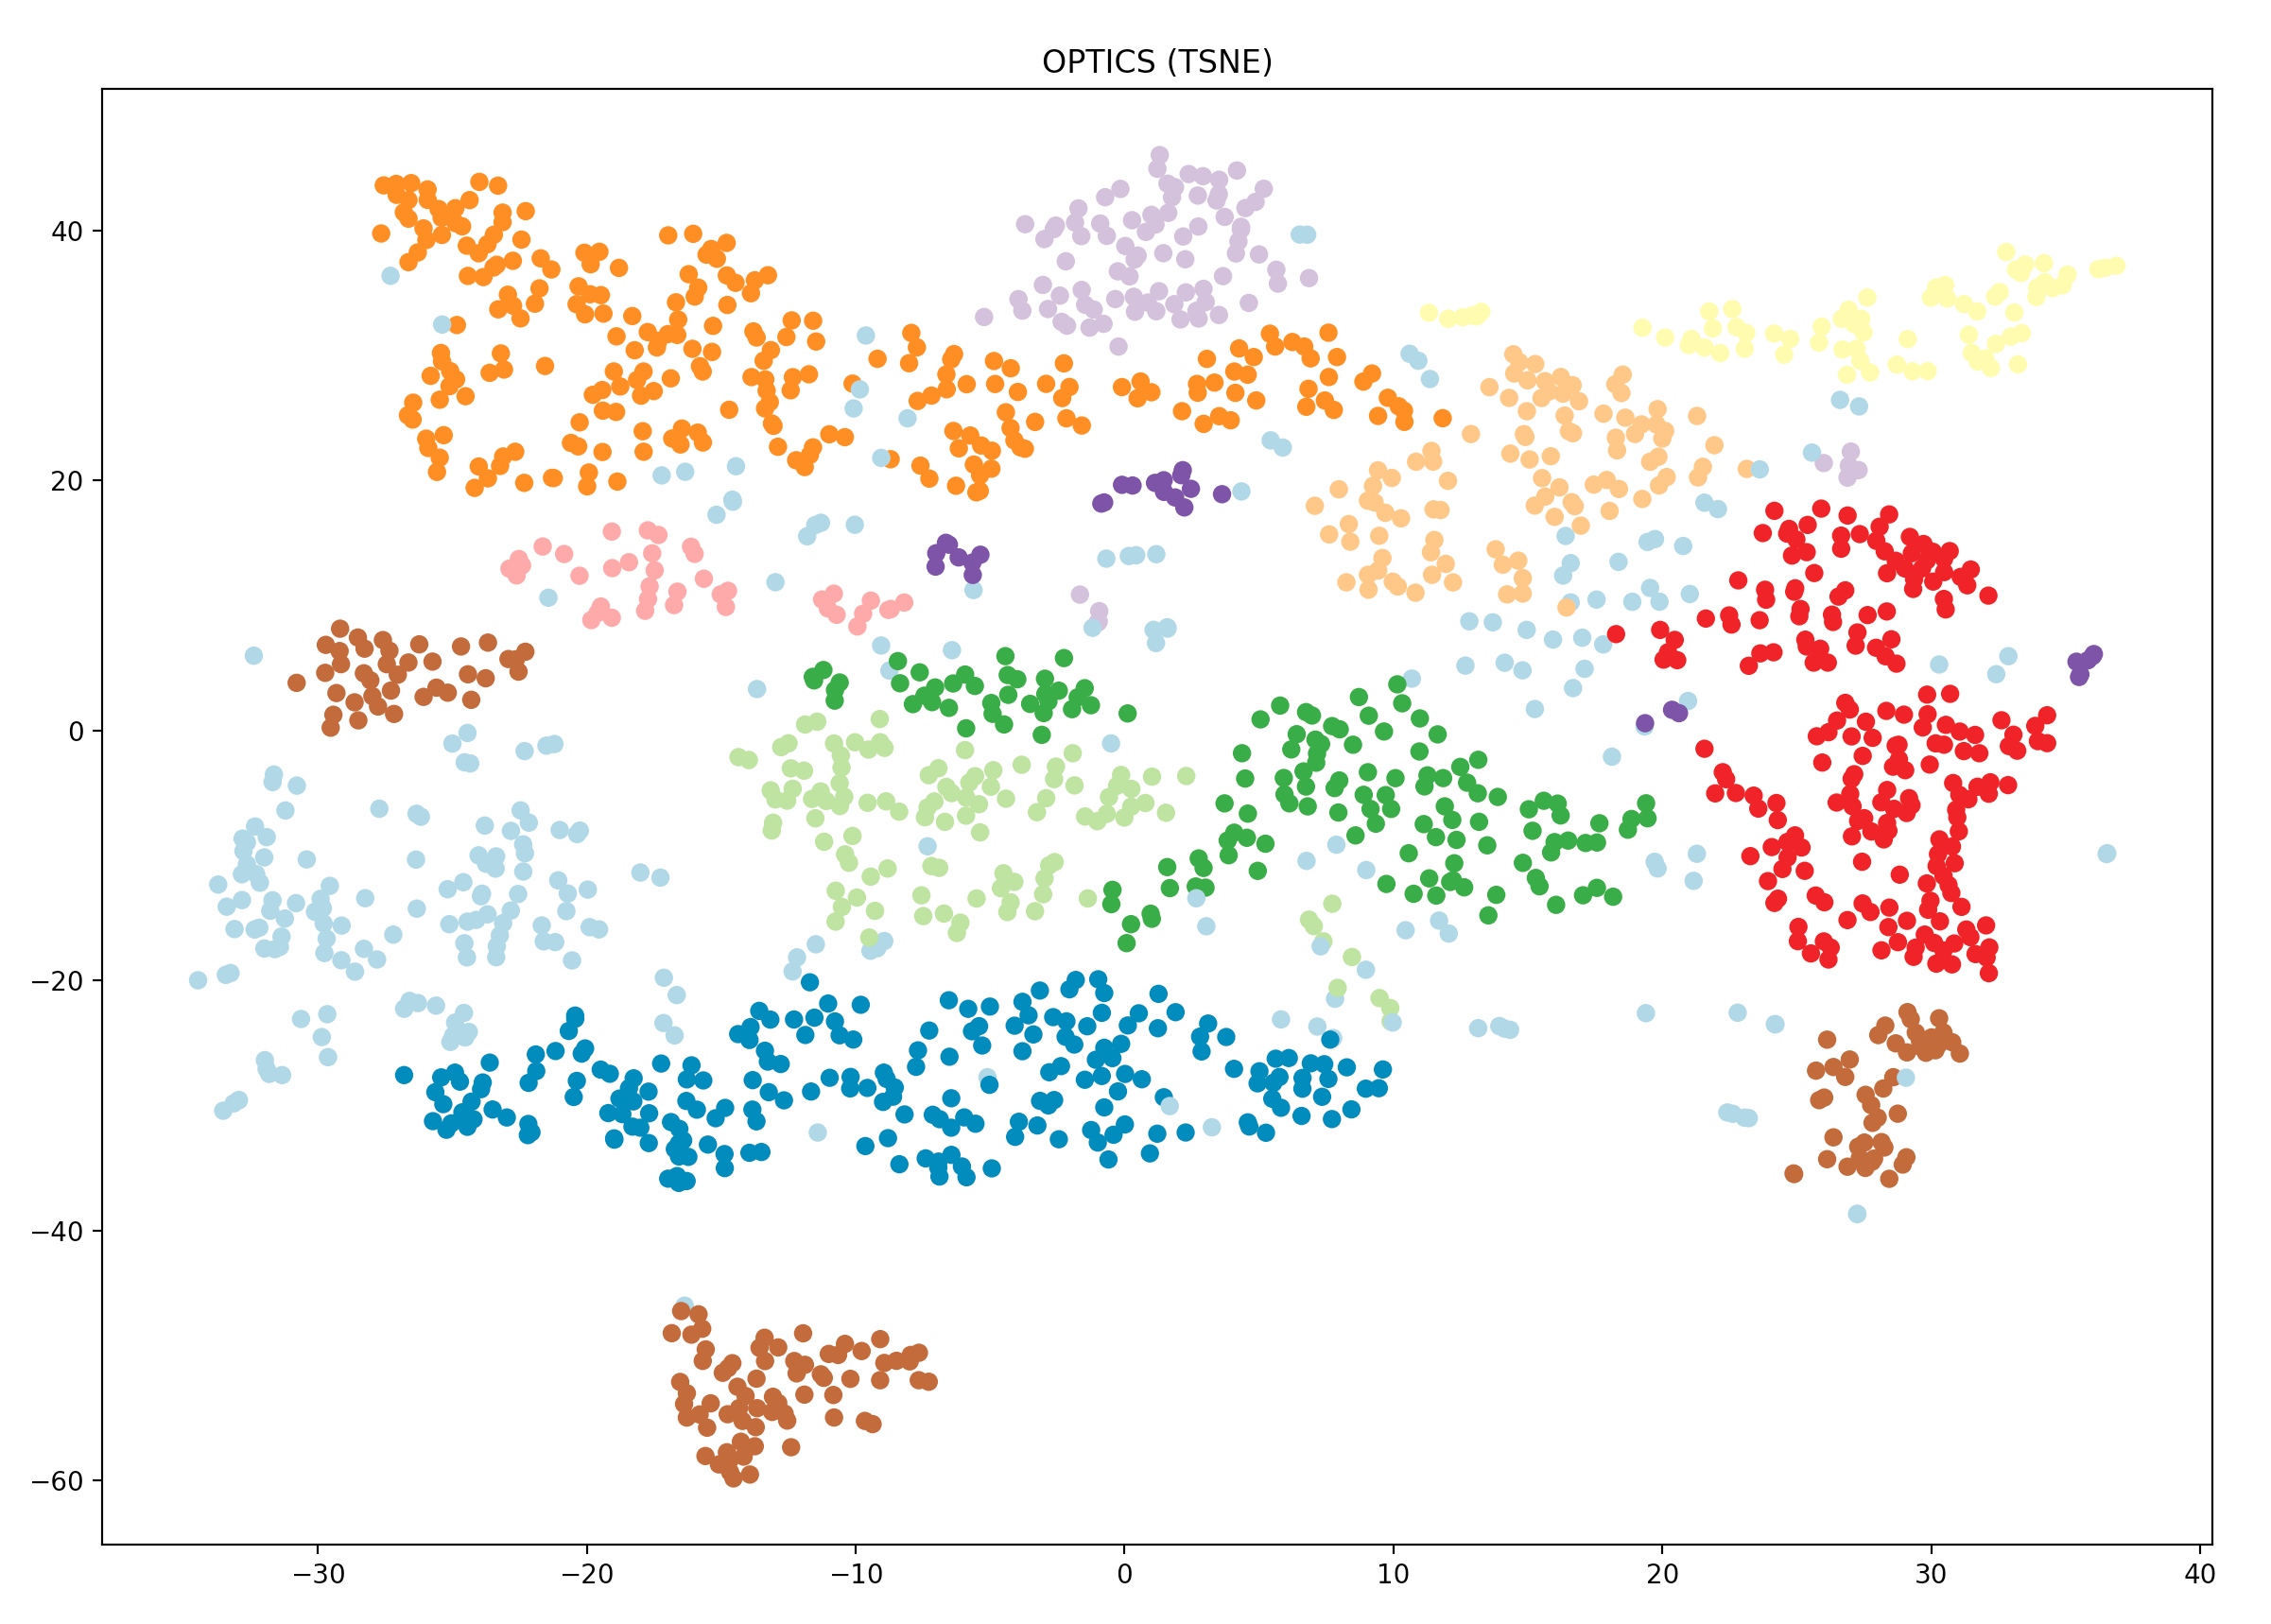
\includegraphics[width=0.9\textwidth]{./images/clusteringResults/1h-2-OPTICS.png}
	\end{subfigure}
	\caption{Comparison of the scatter plots from the DBSCAN (a) and OPTICS (b) clusterings of the average of the 1st column and 2nd column, so the first \textbf{30 minutes} (1h data files: 15 minutes \& 30 minutes).}
  \label{figure:finalClustering1h-2}
\end{figure}

\begin{figure}[H]
	\centering
	\begin{subfigure}{.5\textwidth}
    \centering
    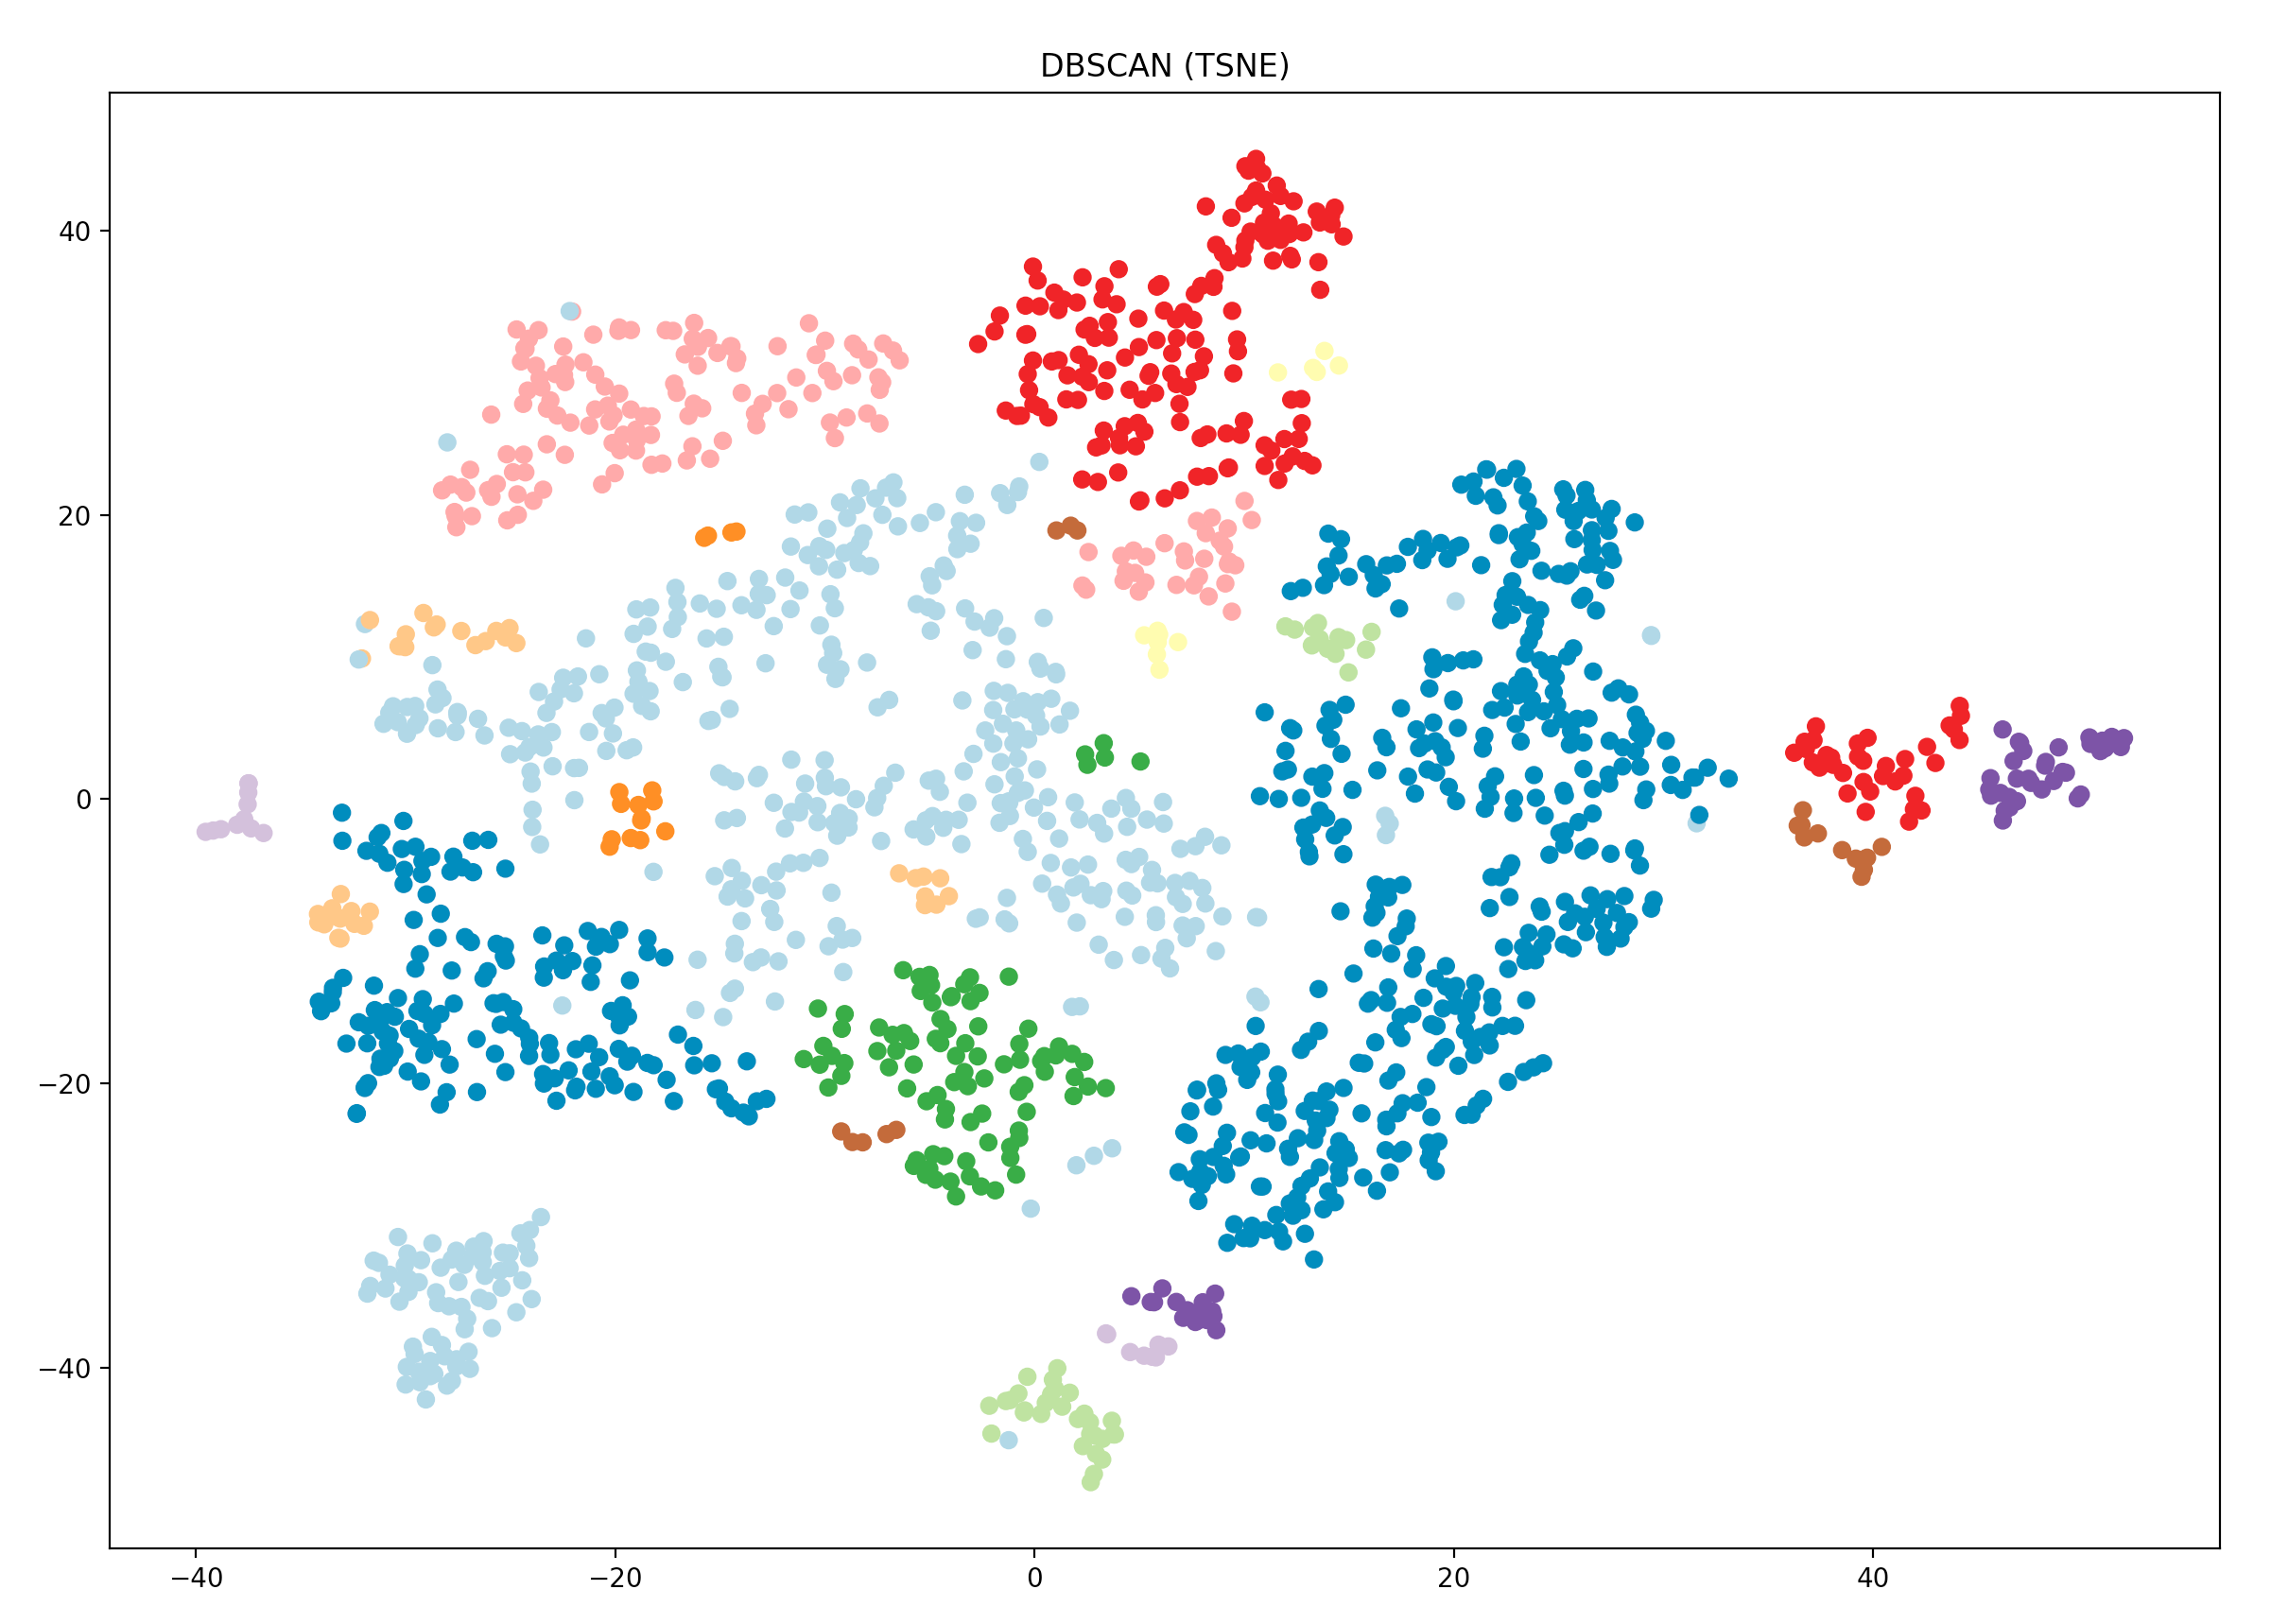
\includegraphics[width=0.9\textwidth]{./images/clusteringResults/1h-3-DBSCAN.png}
  \end{subfigure}%
  \begin{subfigure}{.5\textwidth}
    \centering
    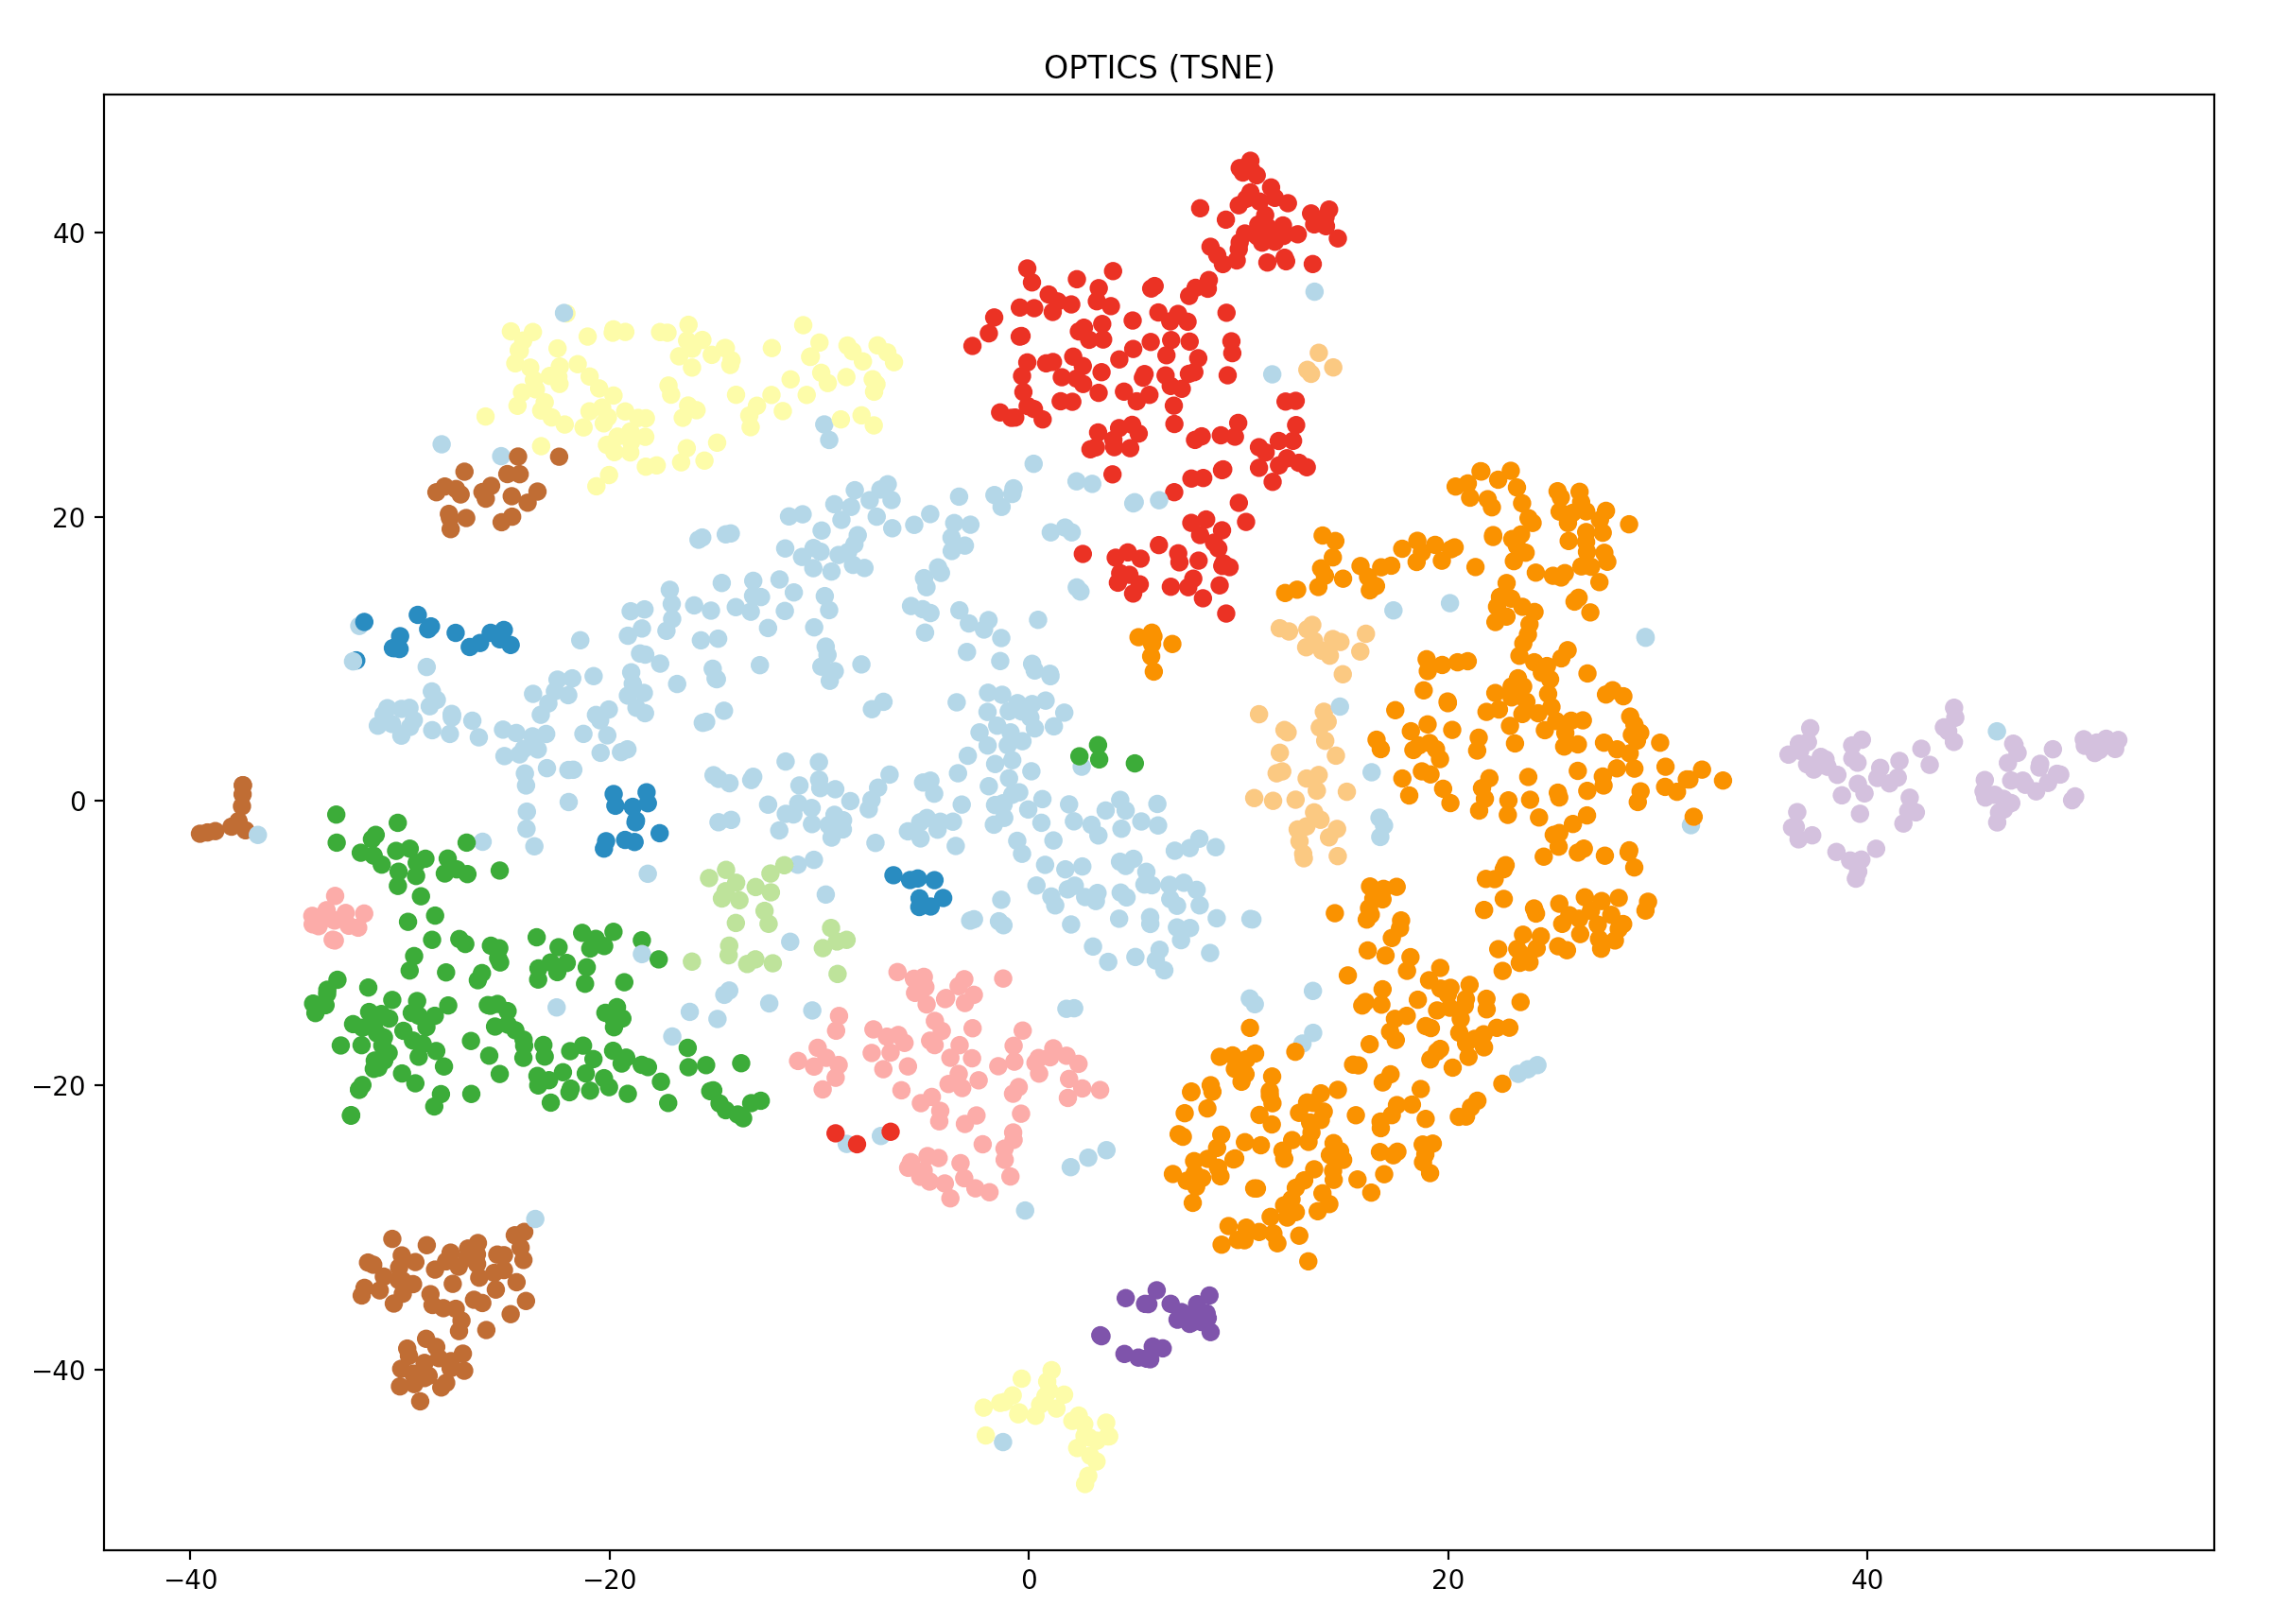
\includegraphics[width=0.9\textwidth]{./images/clusteringResults/1h-3-OPTICS.png}
	\end{subfigure}
	\caption{Comparison of the scatter plots from the DBSCAN (a) and OPTICS (b) clusterings of the average of the 1st column to the 3rd column, so the first \textbf{45 minutes} (1h data files: 15 minutes, 30 minutes \& 45 minutes).}
  \label{figure:finalClustering1h-3}
\end{figure}

\begin{figure}[H]
	\centering
	\begin{subfigure}{.5\textwidth}
    \centering
    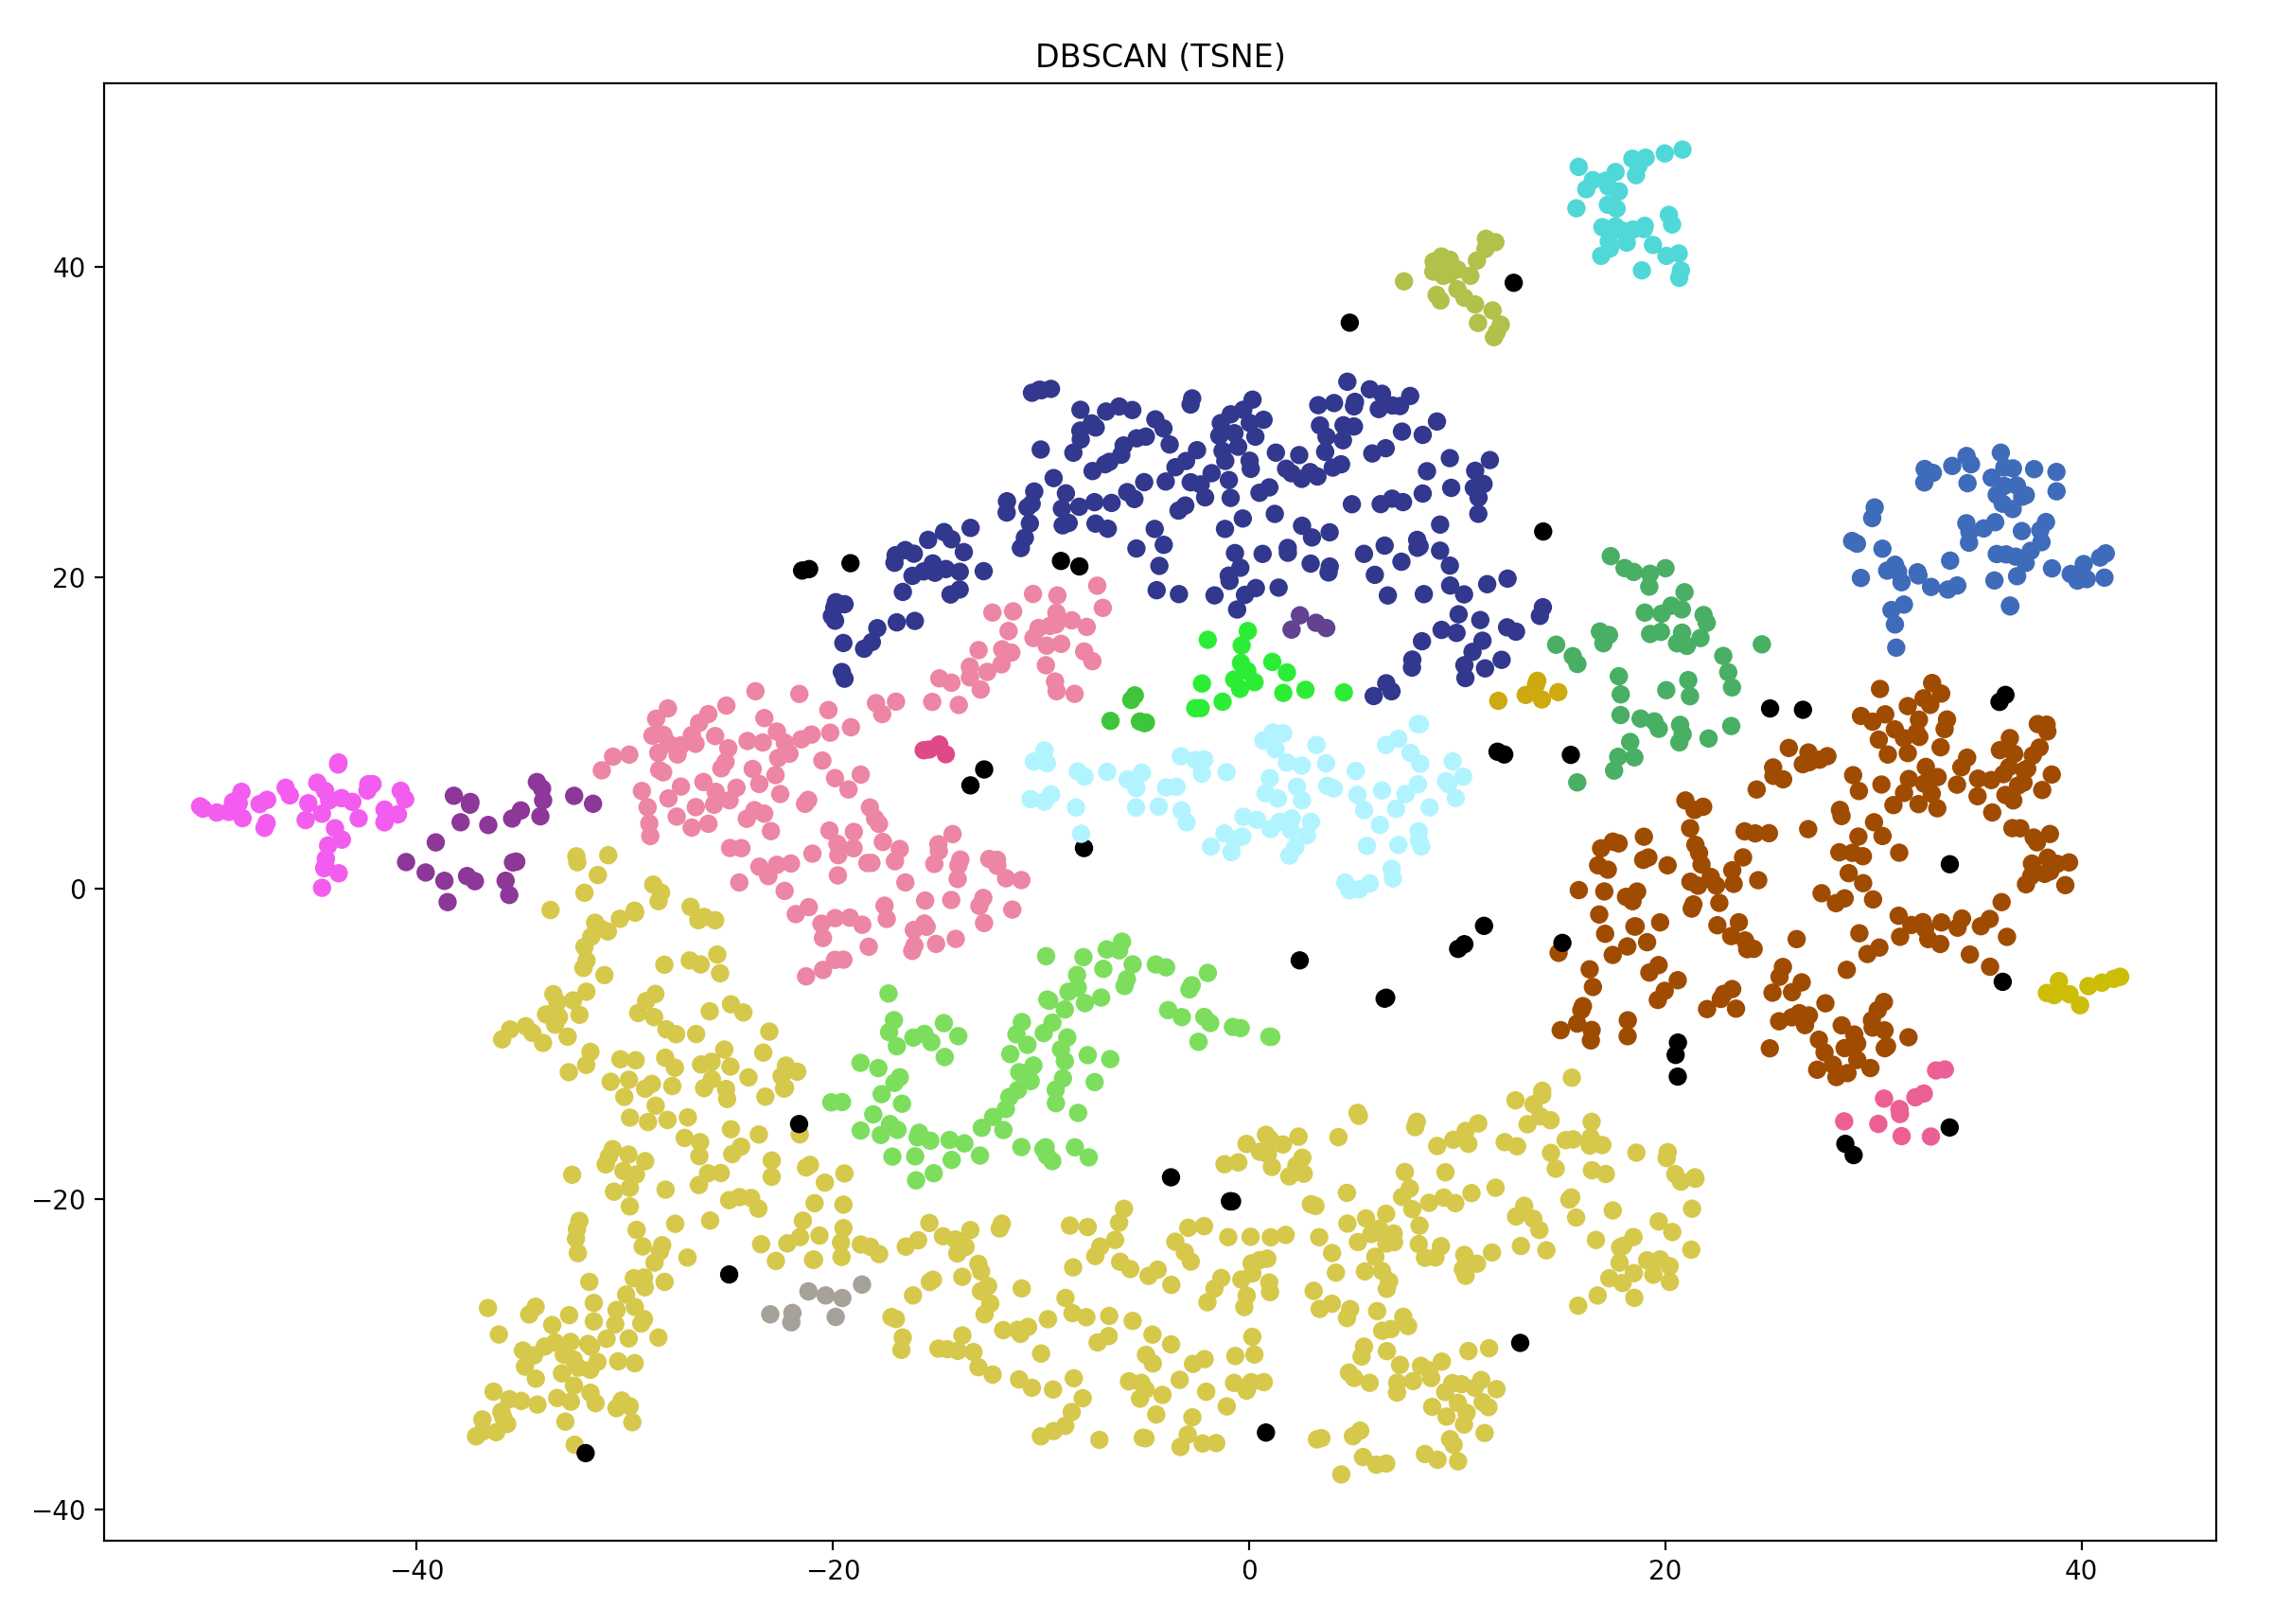
\includegraphics[width=0.9\textwidth]{./images/clusteringResults/1h-4-DBSCAN.png}
  \end{subfigure}%
  \begin{subfigure}{.5\textwidth}
    \centering
    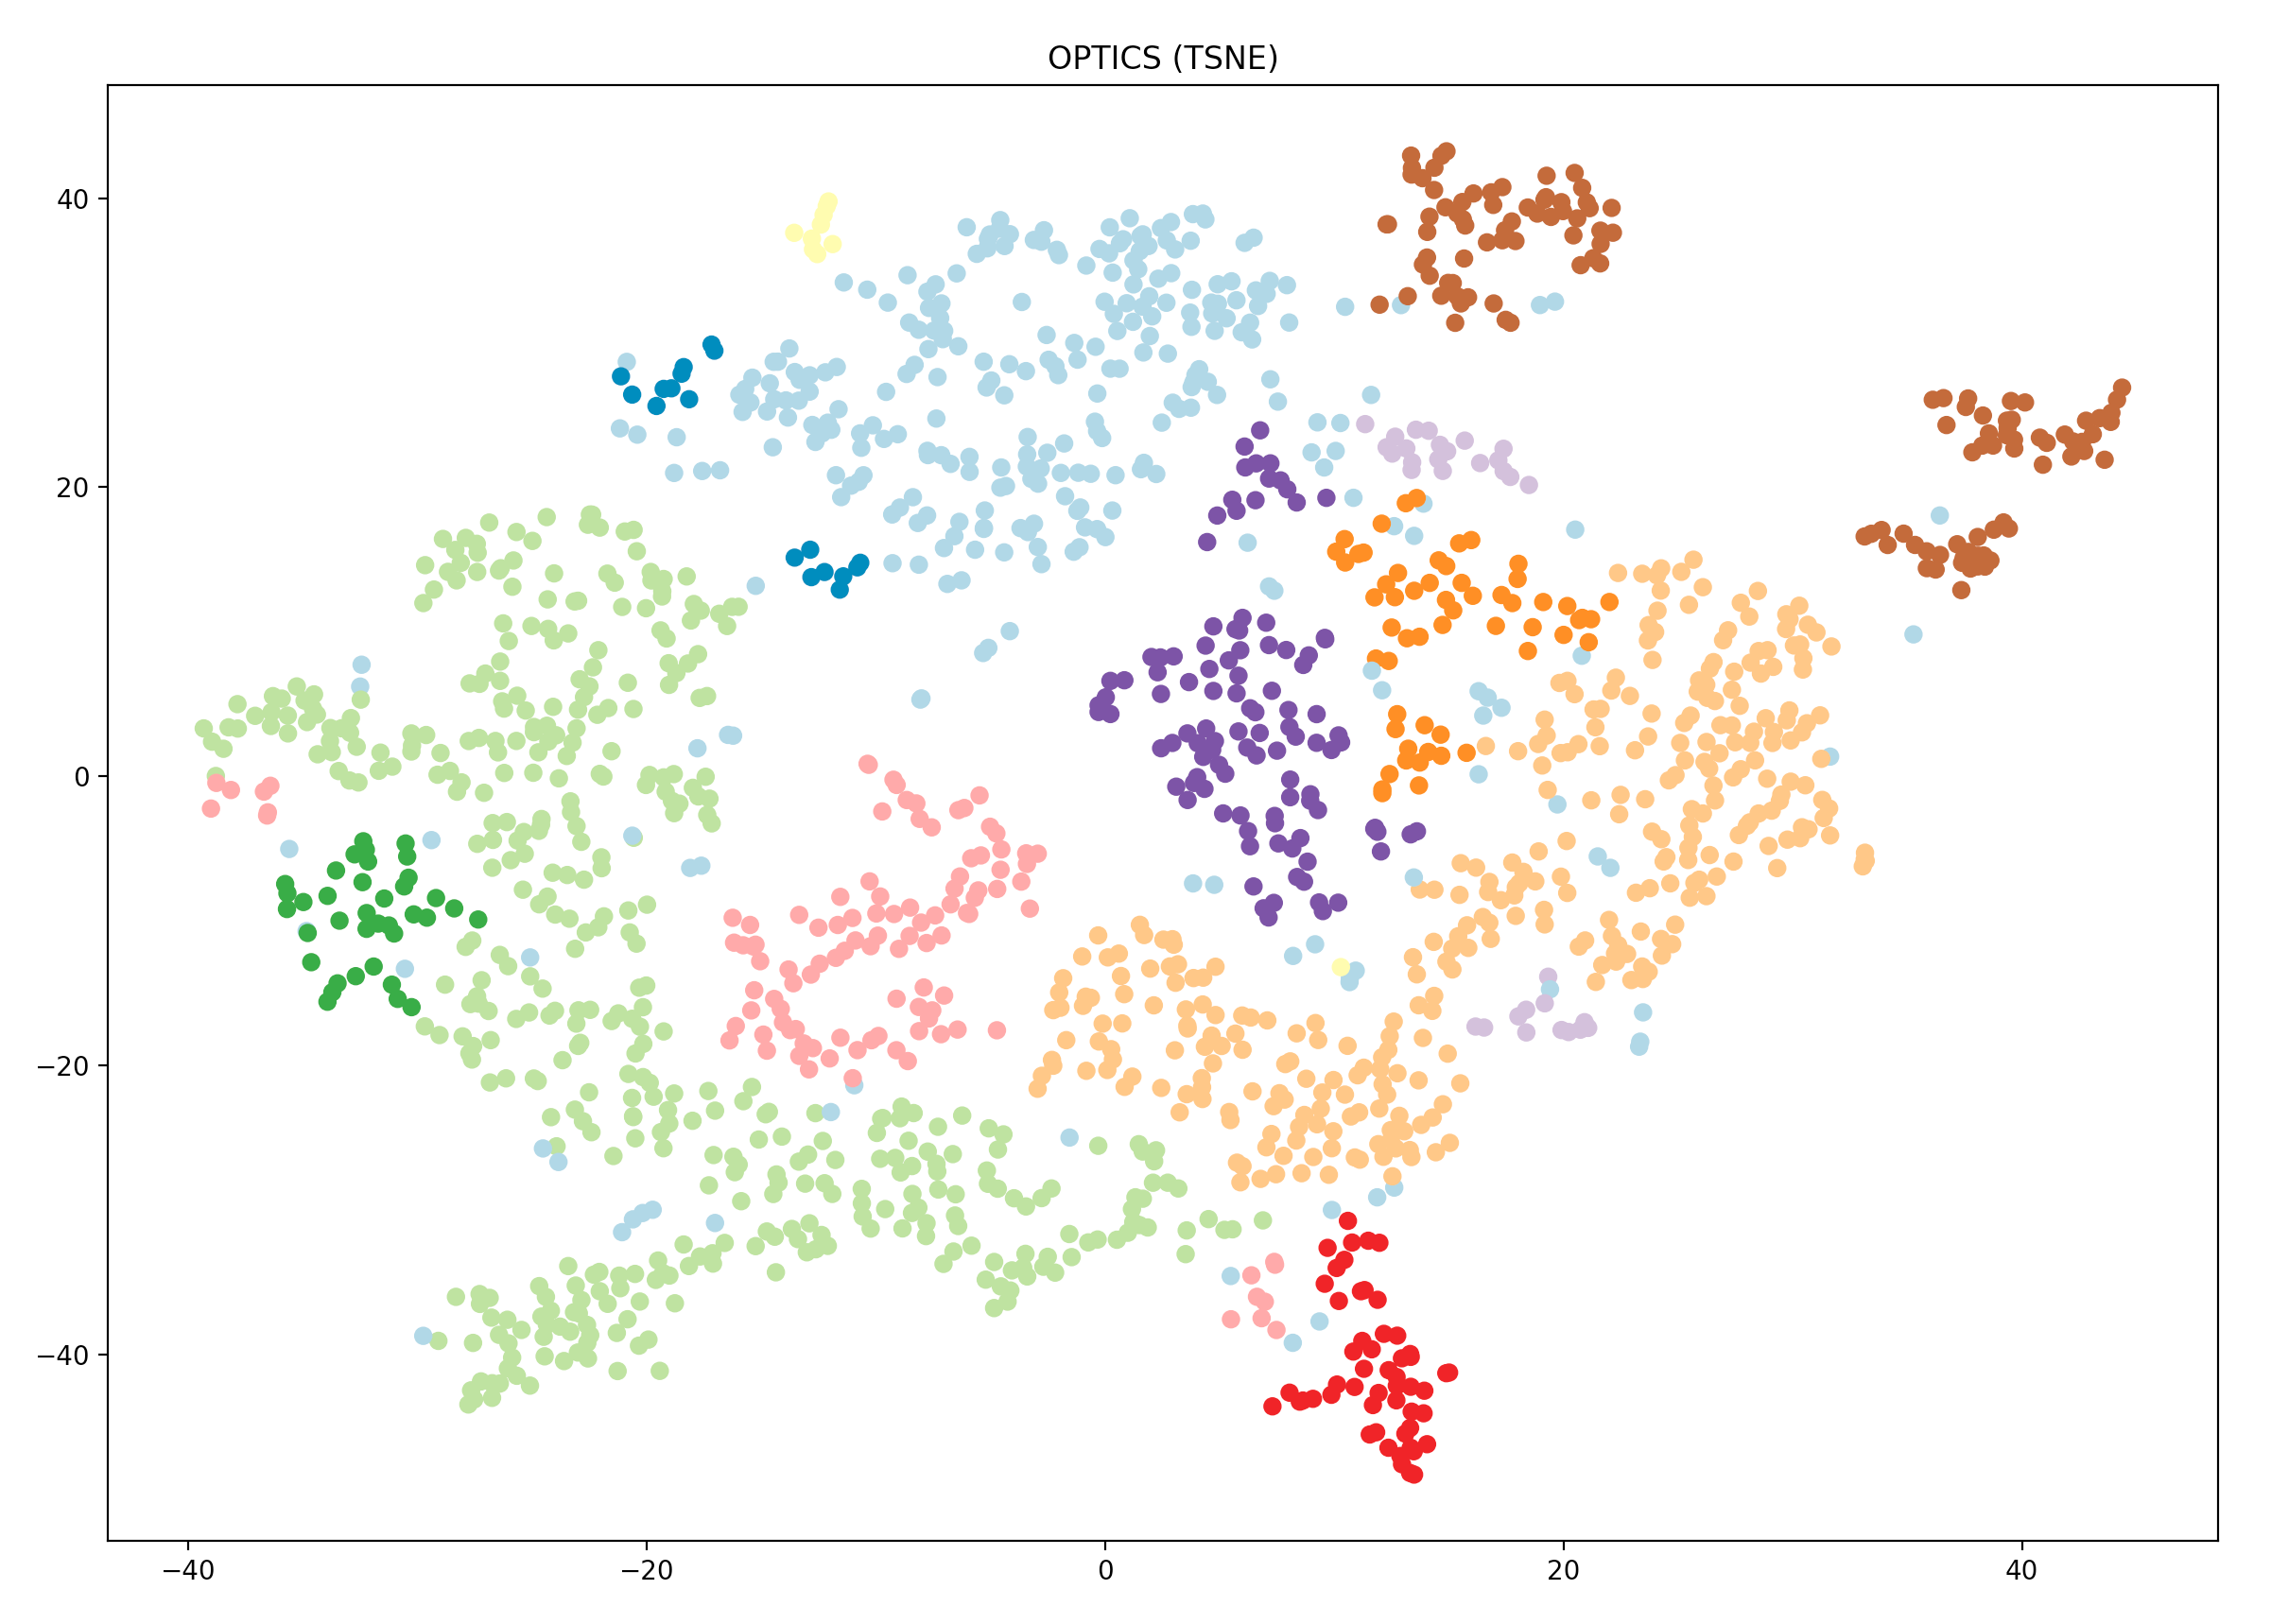
\includegraphics[width=0.9\textwidth]{./images/clusteringResults/1h-4-OPTICS.png}
	\end{subfigure}
	\caption{Comparison of the scatter plots from the DBSCAN (a) and OPTICS (b) clusterings of the average of the 1st column to the 4th column, so the whole \textbf{1 hour} (1h data files: 15 minutes, 30 minutes, 45 minutes \& 1 hour).}
  \label{figure:finalClustering1h-4}
\end{figure}









\subsubsection{3h aggregated data files}

\begin{figure}[H]
	\centering
	\begin{subfigure}{.5\textwidth}
    \centering
    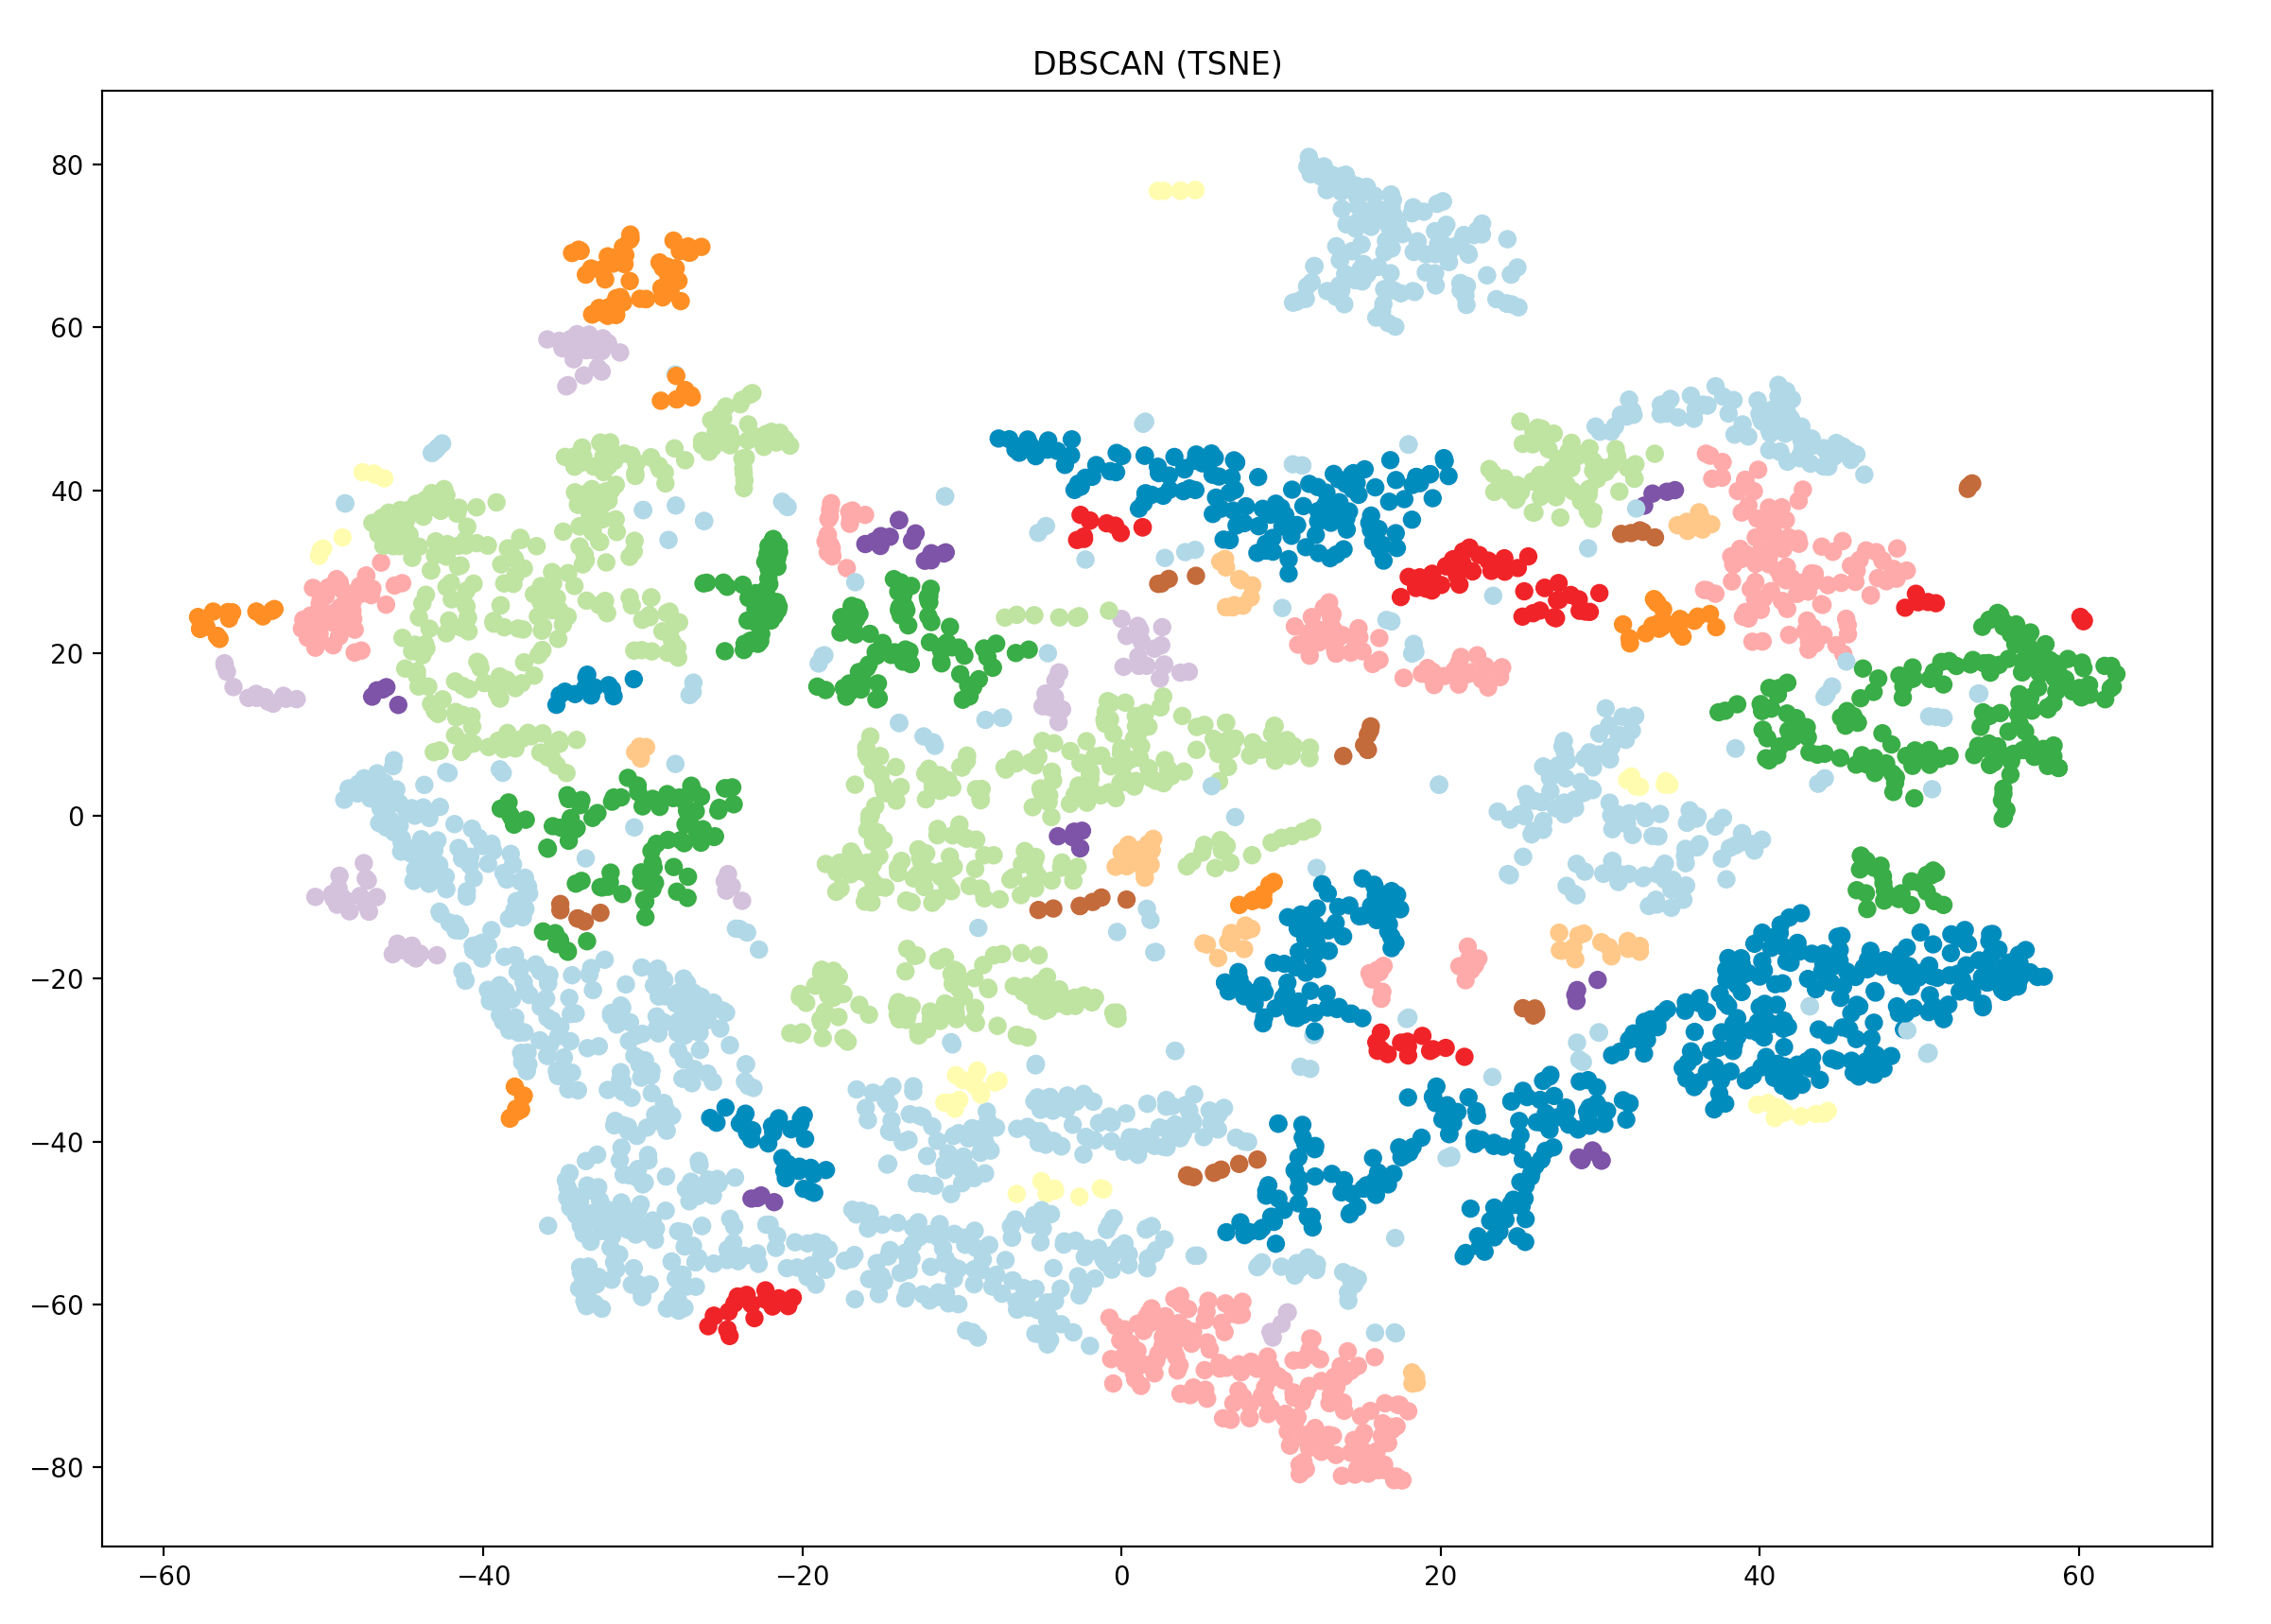
\includegraphics[width=0.9\textwidth]{./images/clusteringResults/3h-1-DBSCAN.png}
  \end{subfigure}%
  \begin{subfigure}{.5\textwidth}
    \centering
    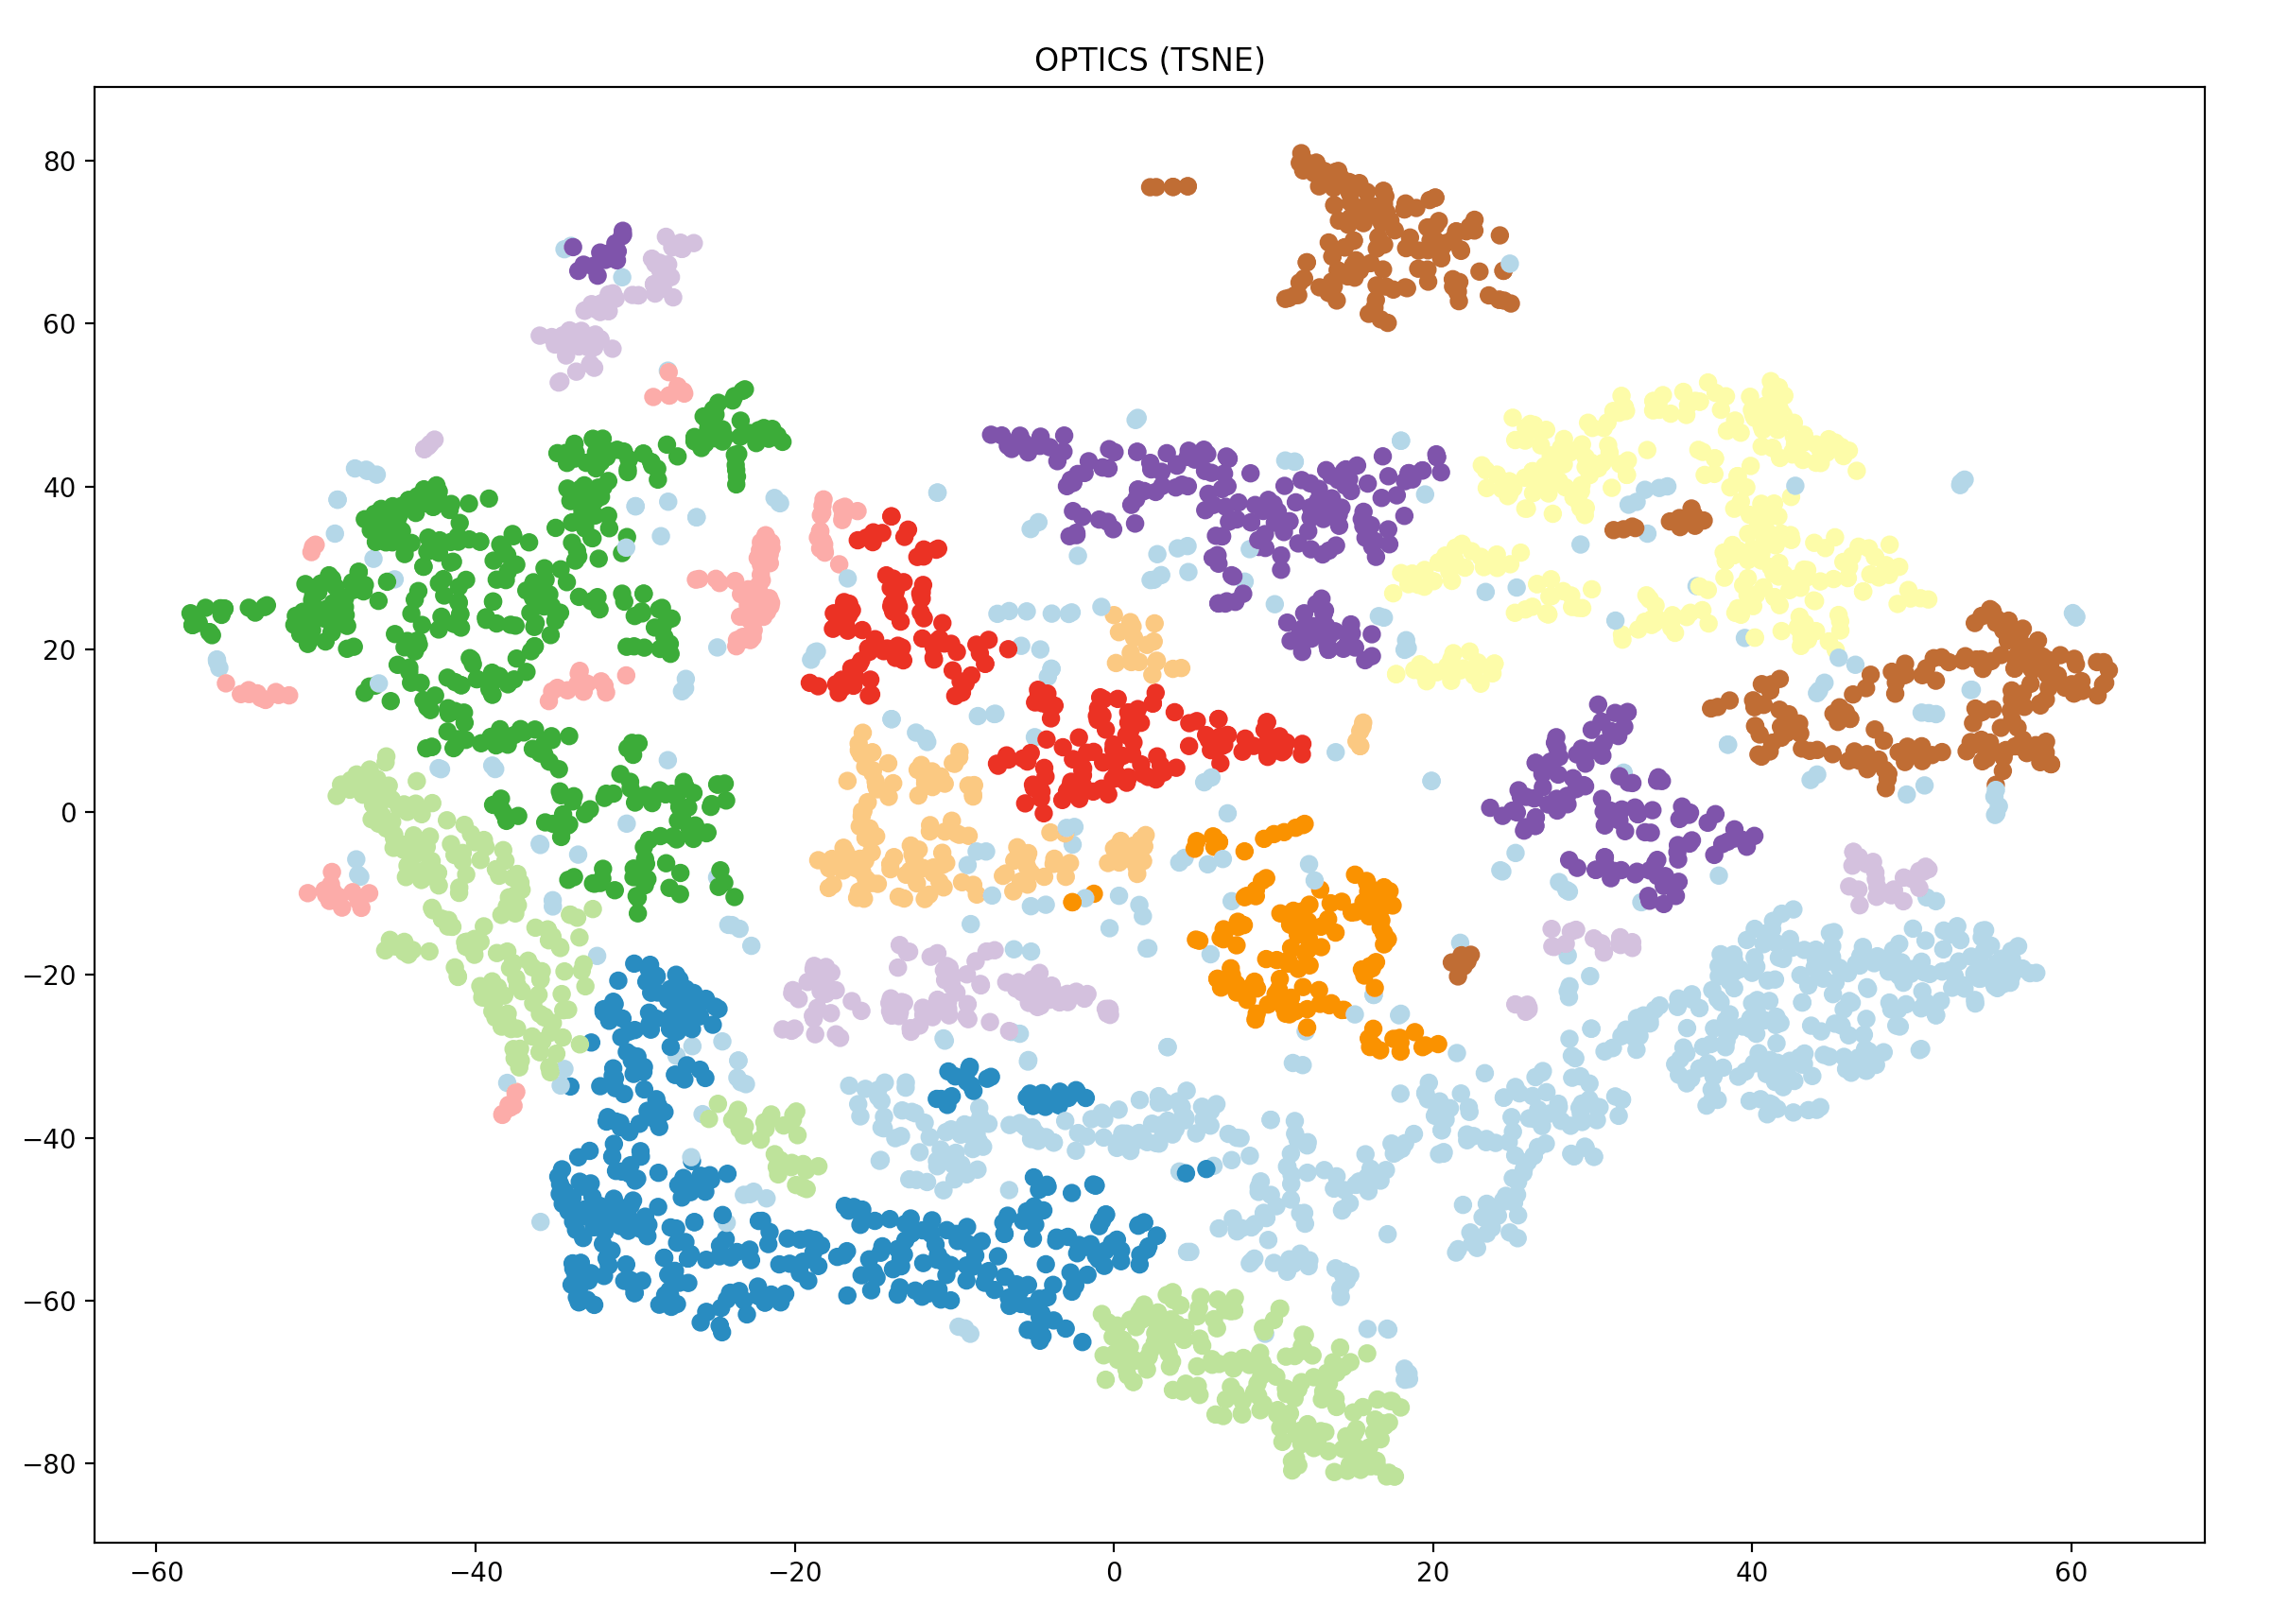
\includegraphics[width=0.9\textwidth]{./images/clusteringResults/3h-1-OPTICS.png}
	\end{subfigure}
	\caption{Comparison of the scatter plots from the DBSCAN (a) and OPTICS (b) clusterings of the 1st column, so the first \textbf{30 minutes} (3h data files: first 30 minutes).}
  \label{figure:finalClustering3h-1}
\end{figure}



\begin{figure}[H]
	\centering
	\begin{subfigure}{.5\textwidth}
    \centering
    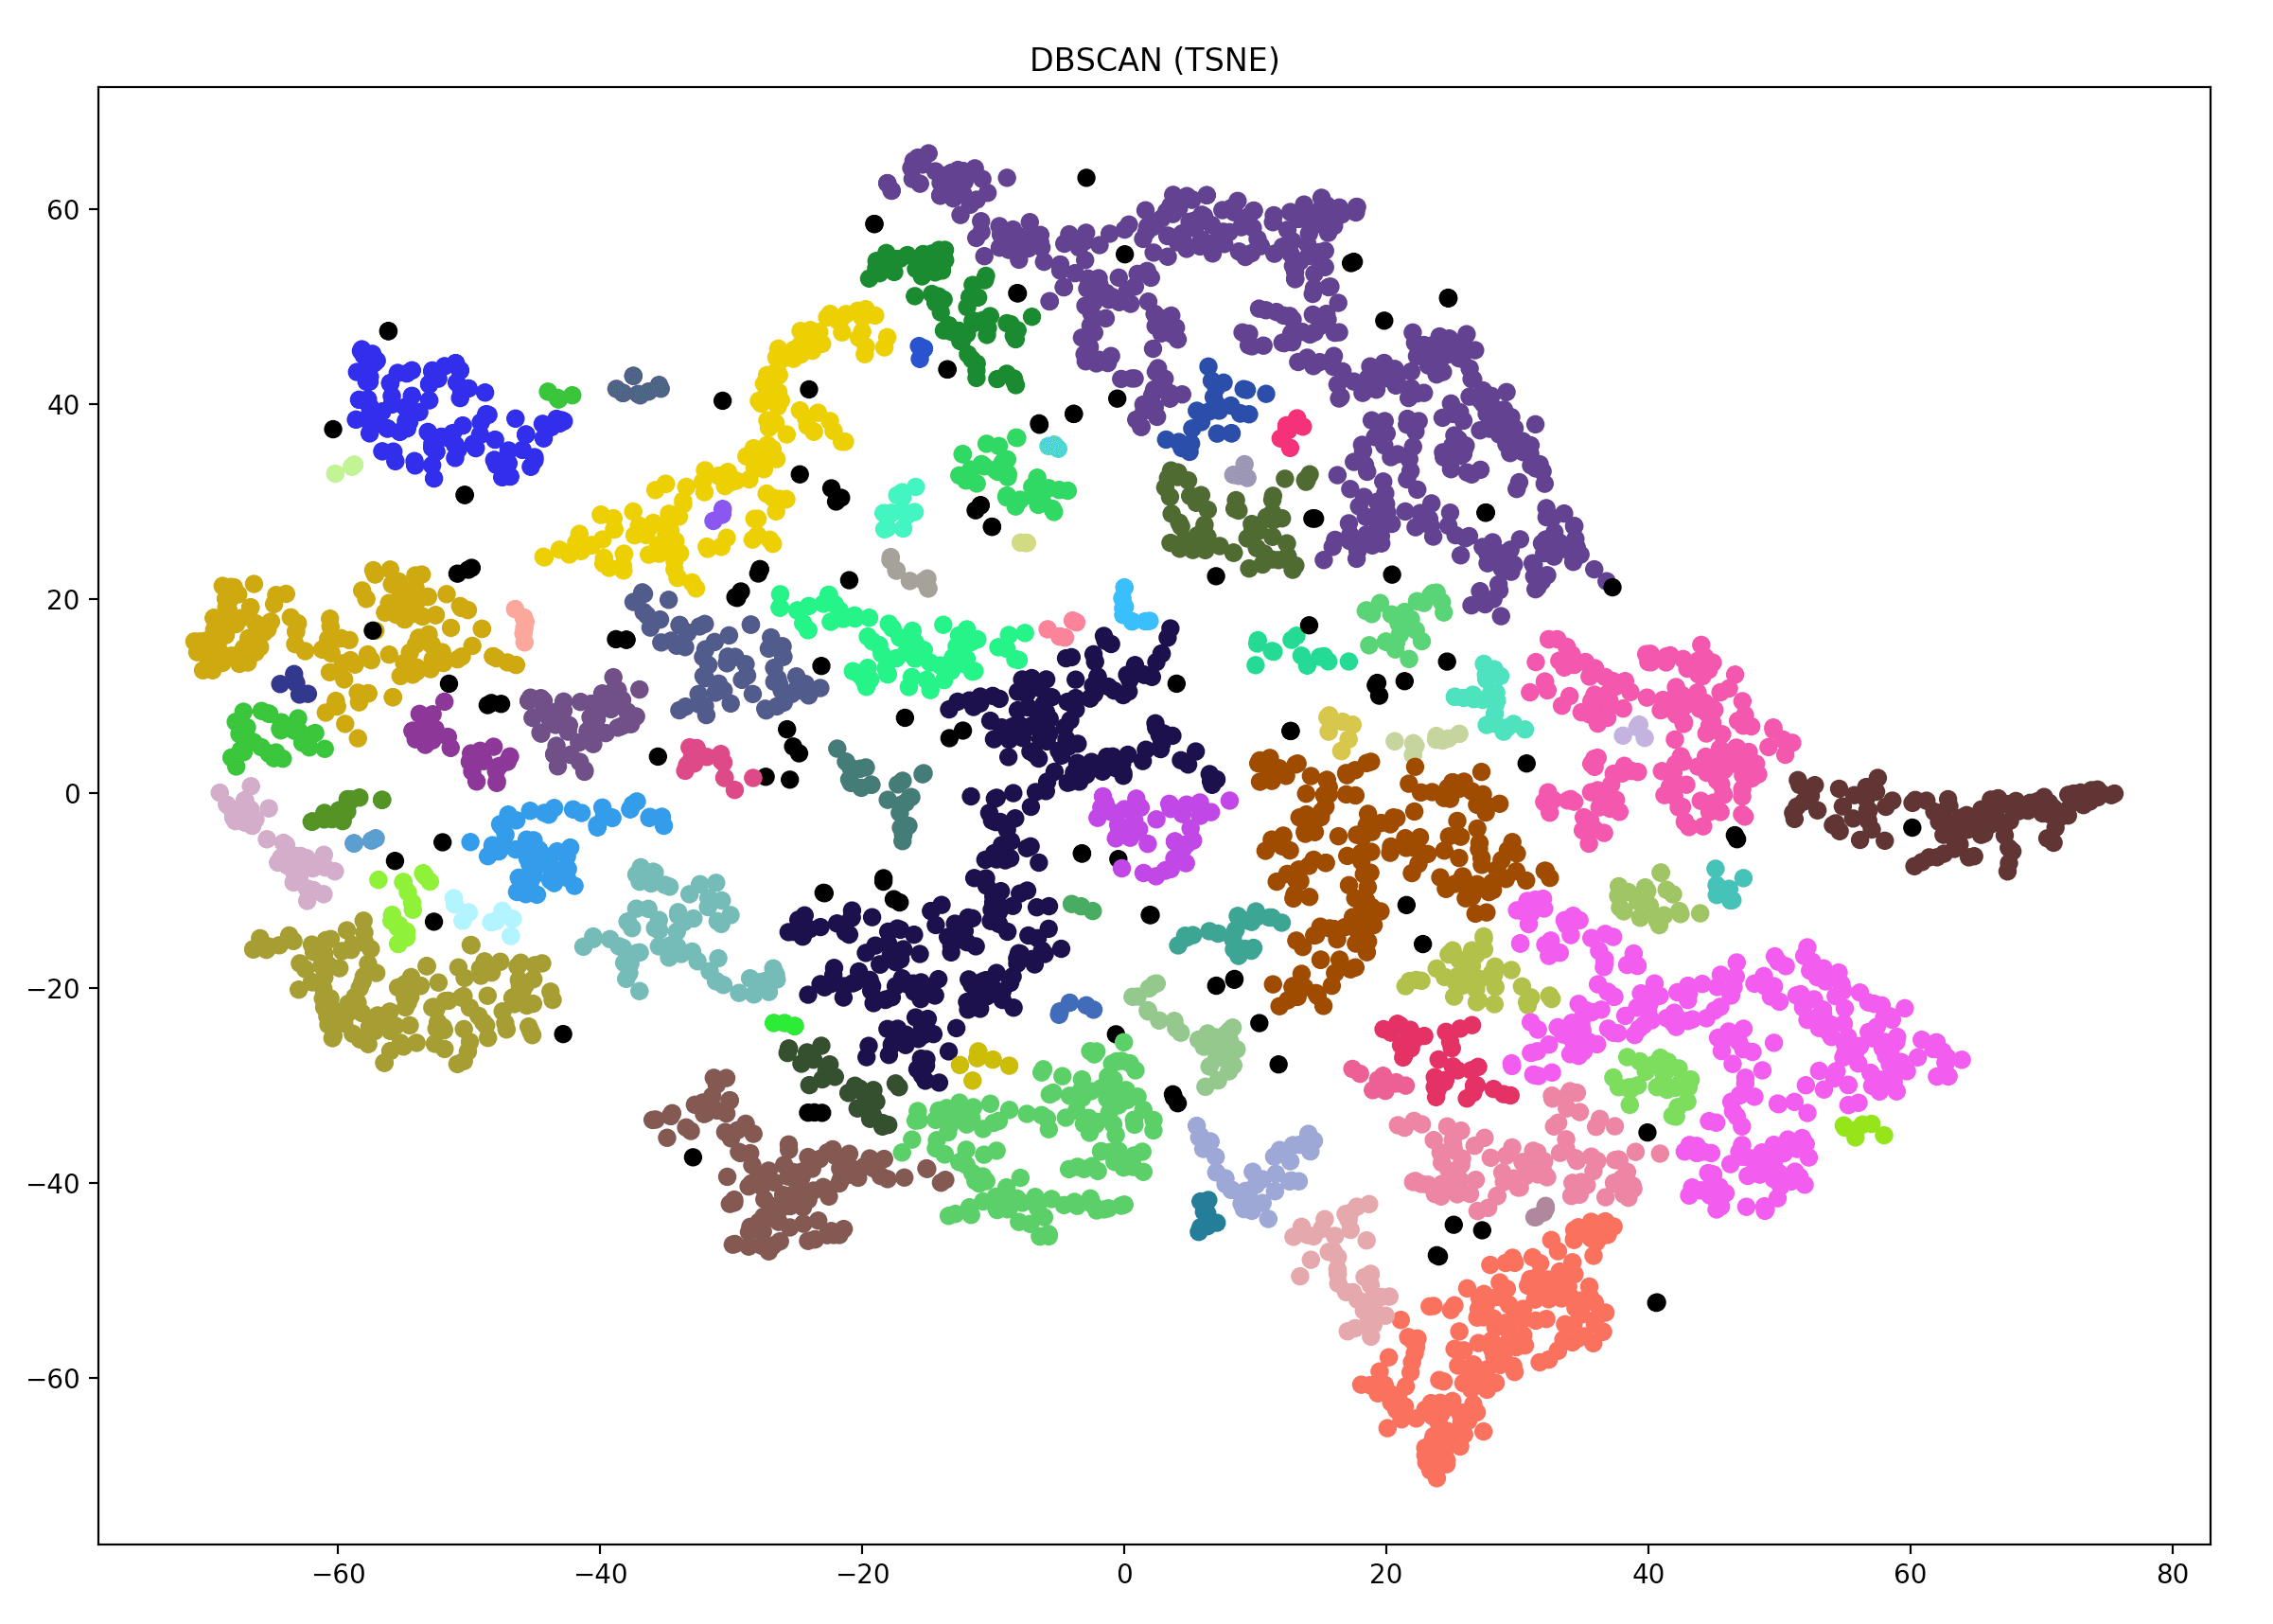
\includegraphics[width=0.9\textwidth]{./images/clusteringResults/3h-2-DBSCAN.png}
  \end{subfigure}%
  \begin{subfigure}{.5\textwidth}
    \centering
    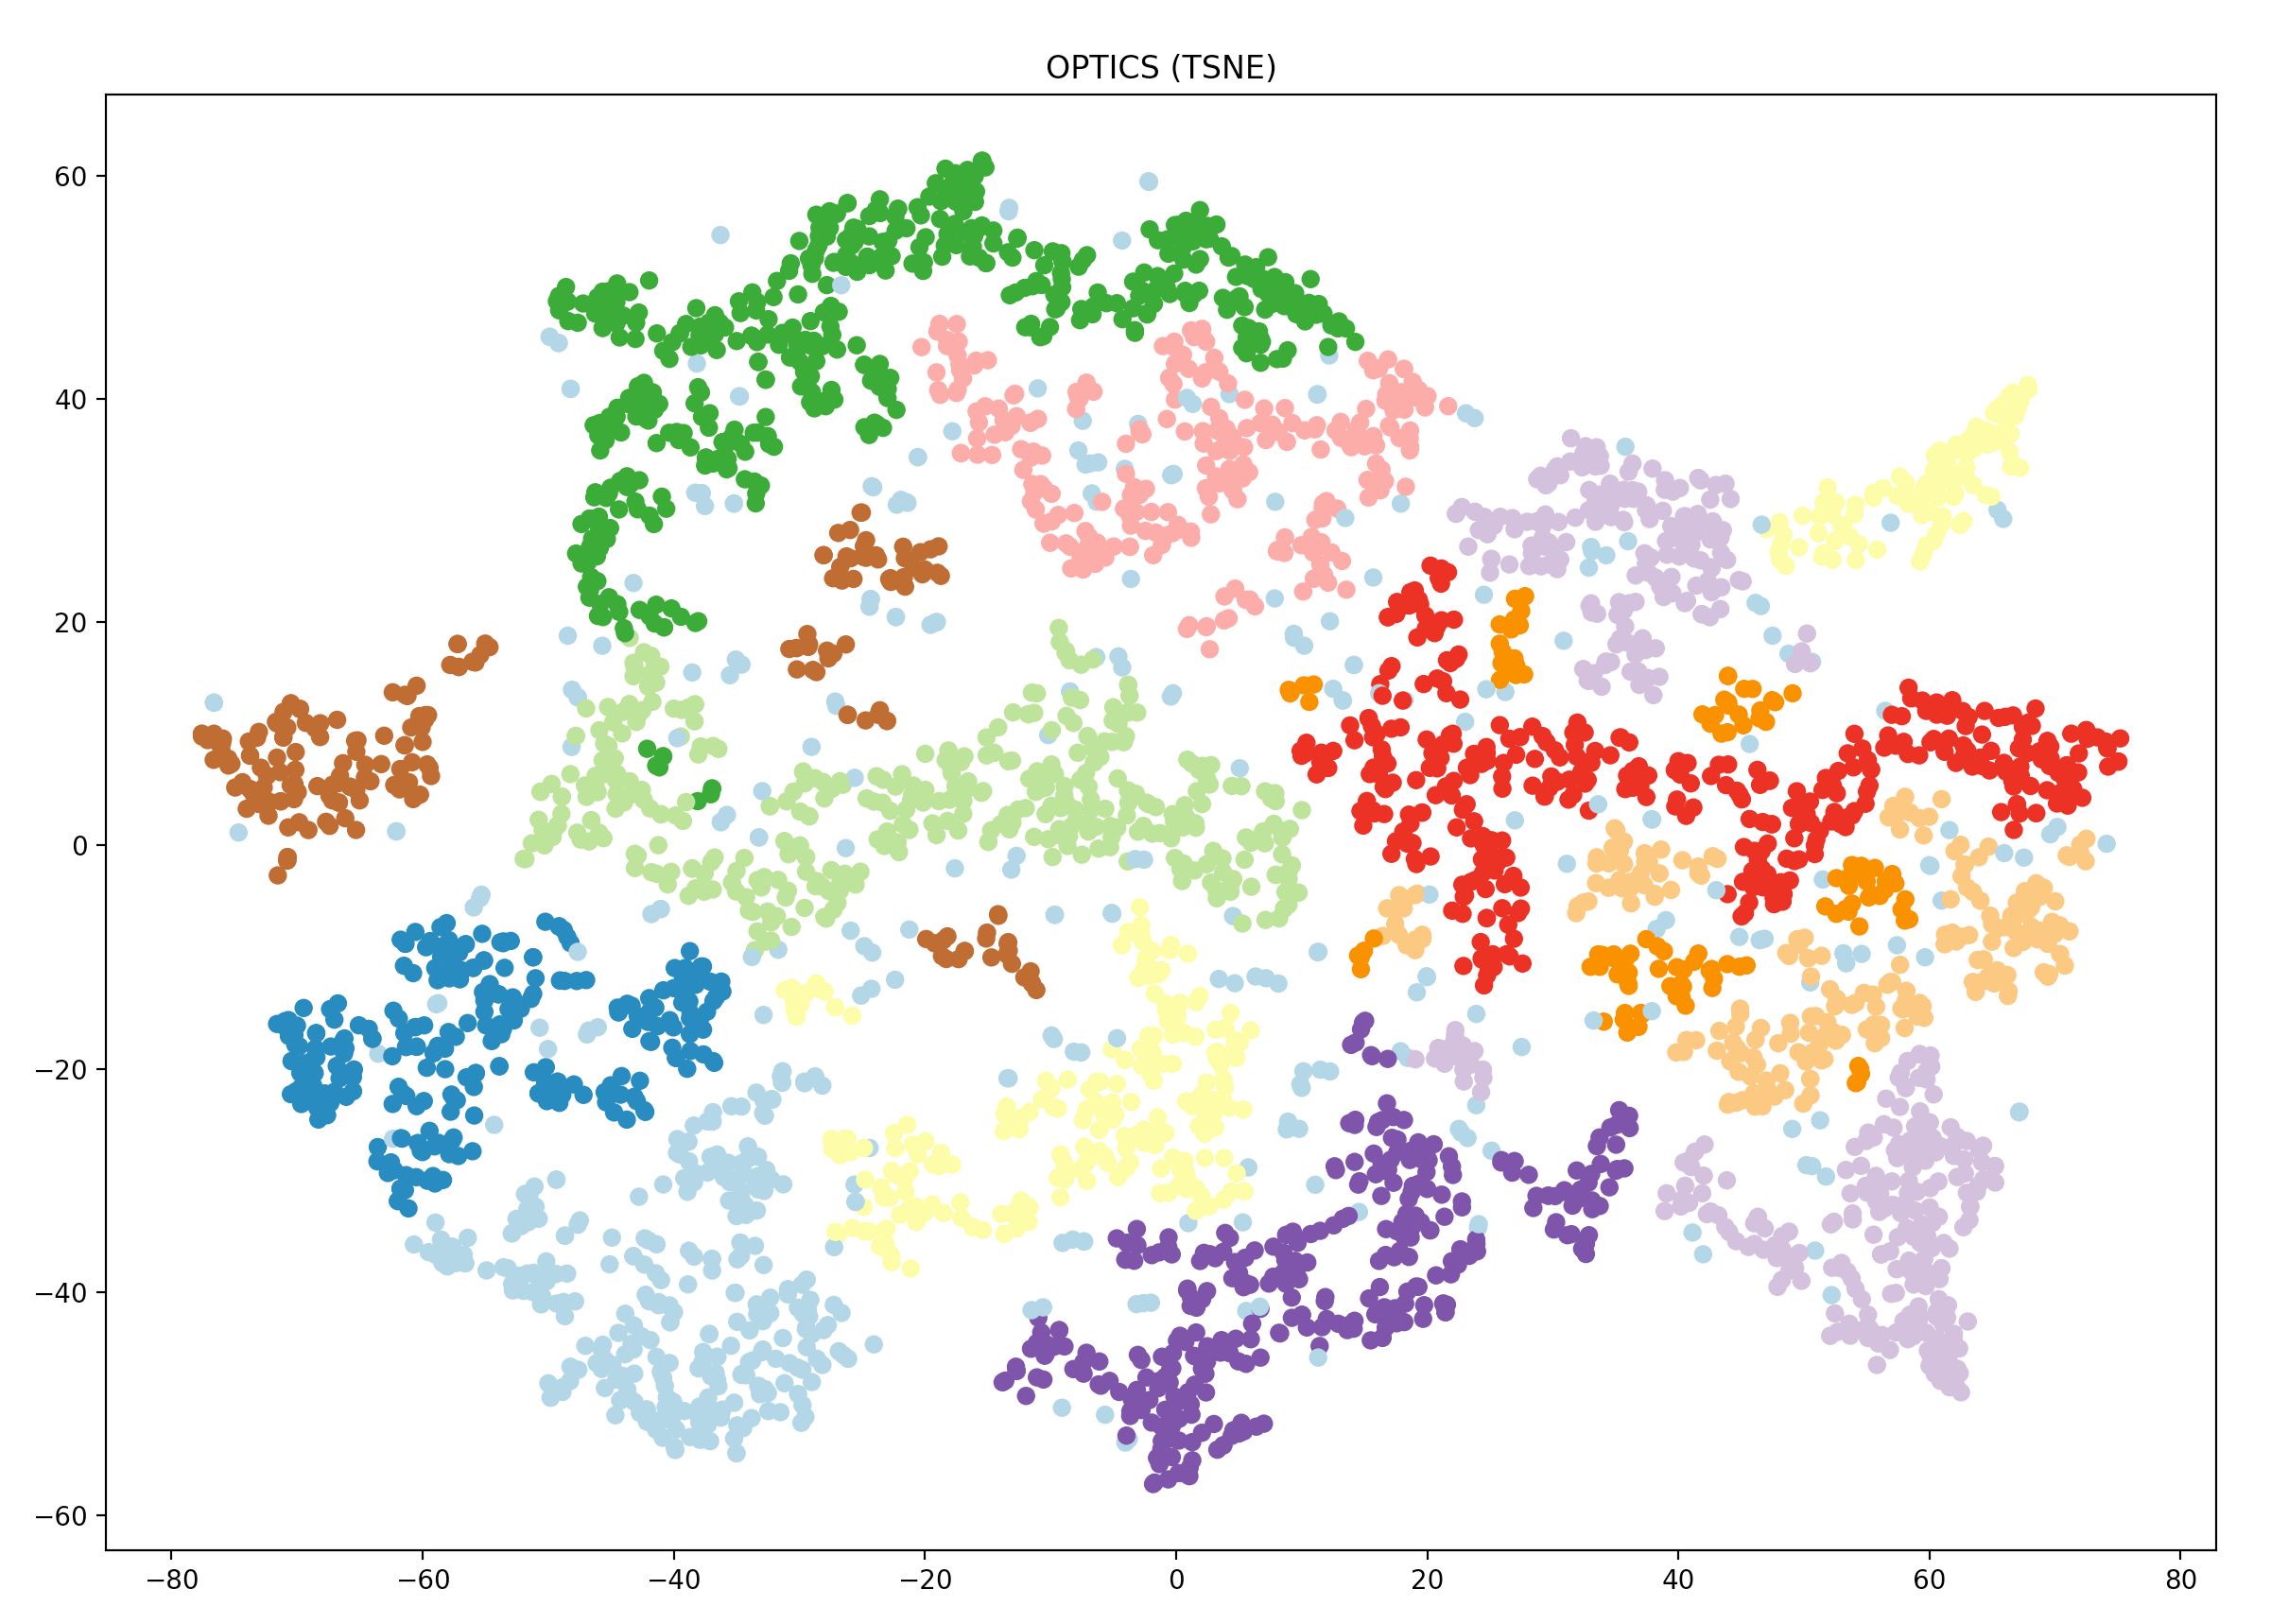
\includegraphics[width=0.9\textwidth]{./images/clusteringResults/3h-2-OPTICS.png}
	\end{subfigure}
	\caption{Comparison of the scatter plots from the DBSCAN (a) and OPTICS (b) clusterings of the average of the 1st column and 2nd column, so the first \textbf{1 hour} (3h data files: 30 minutes \& 1 hour).}
  \label{figure:finalClustering3h-2}
\end{figure}

\begin{figure}[H]
	\centering
	\begin{subfigure}{.5\textwidth}
    \centering
    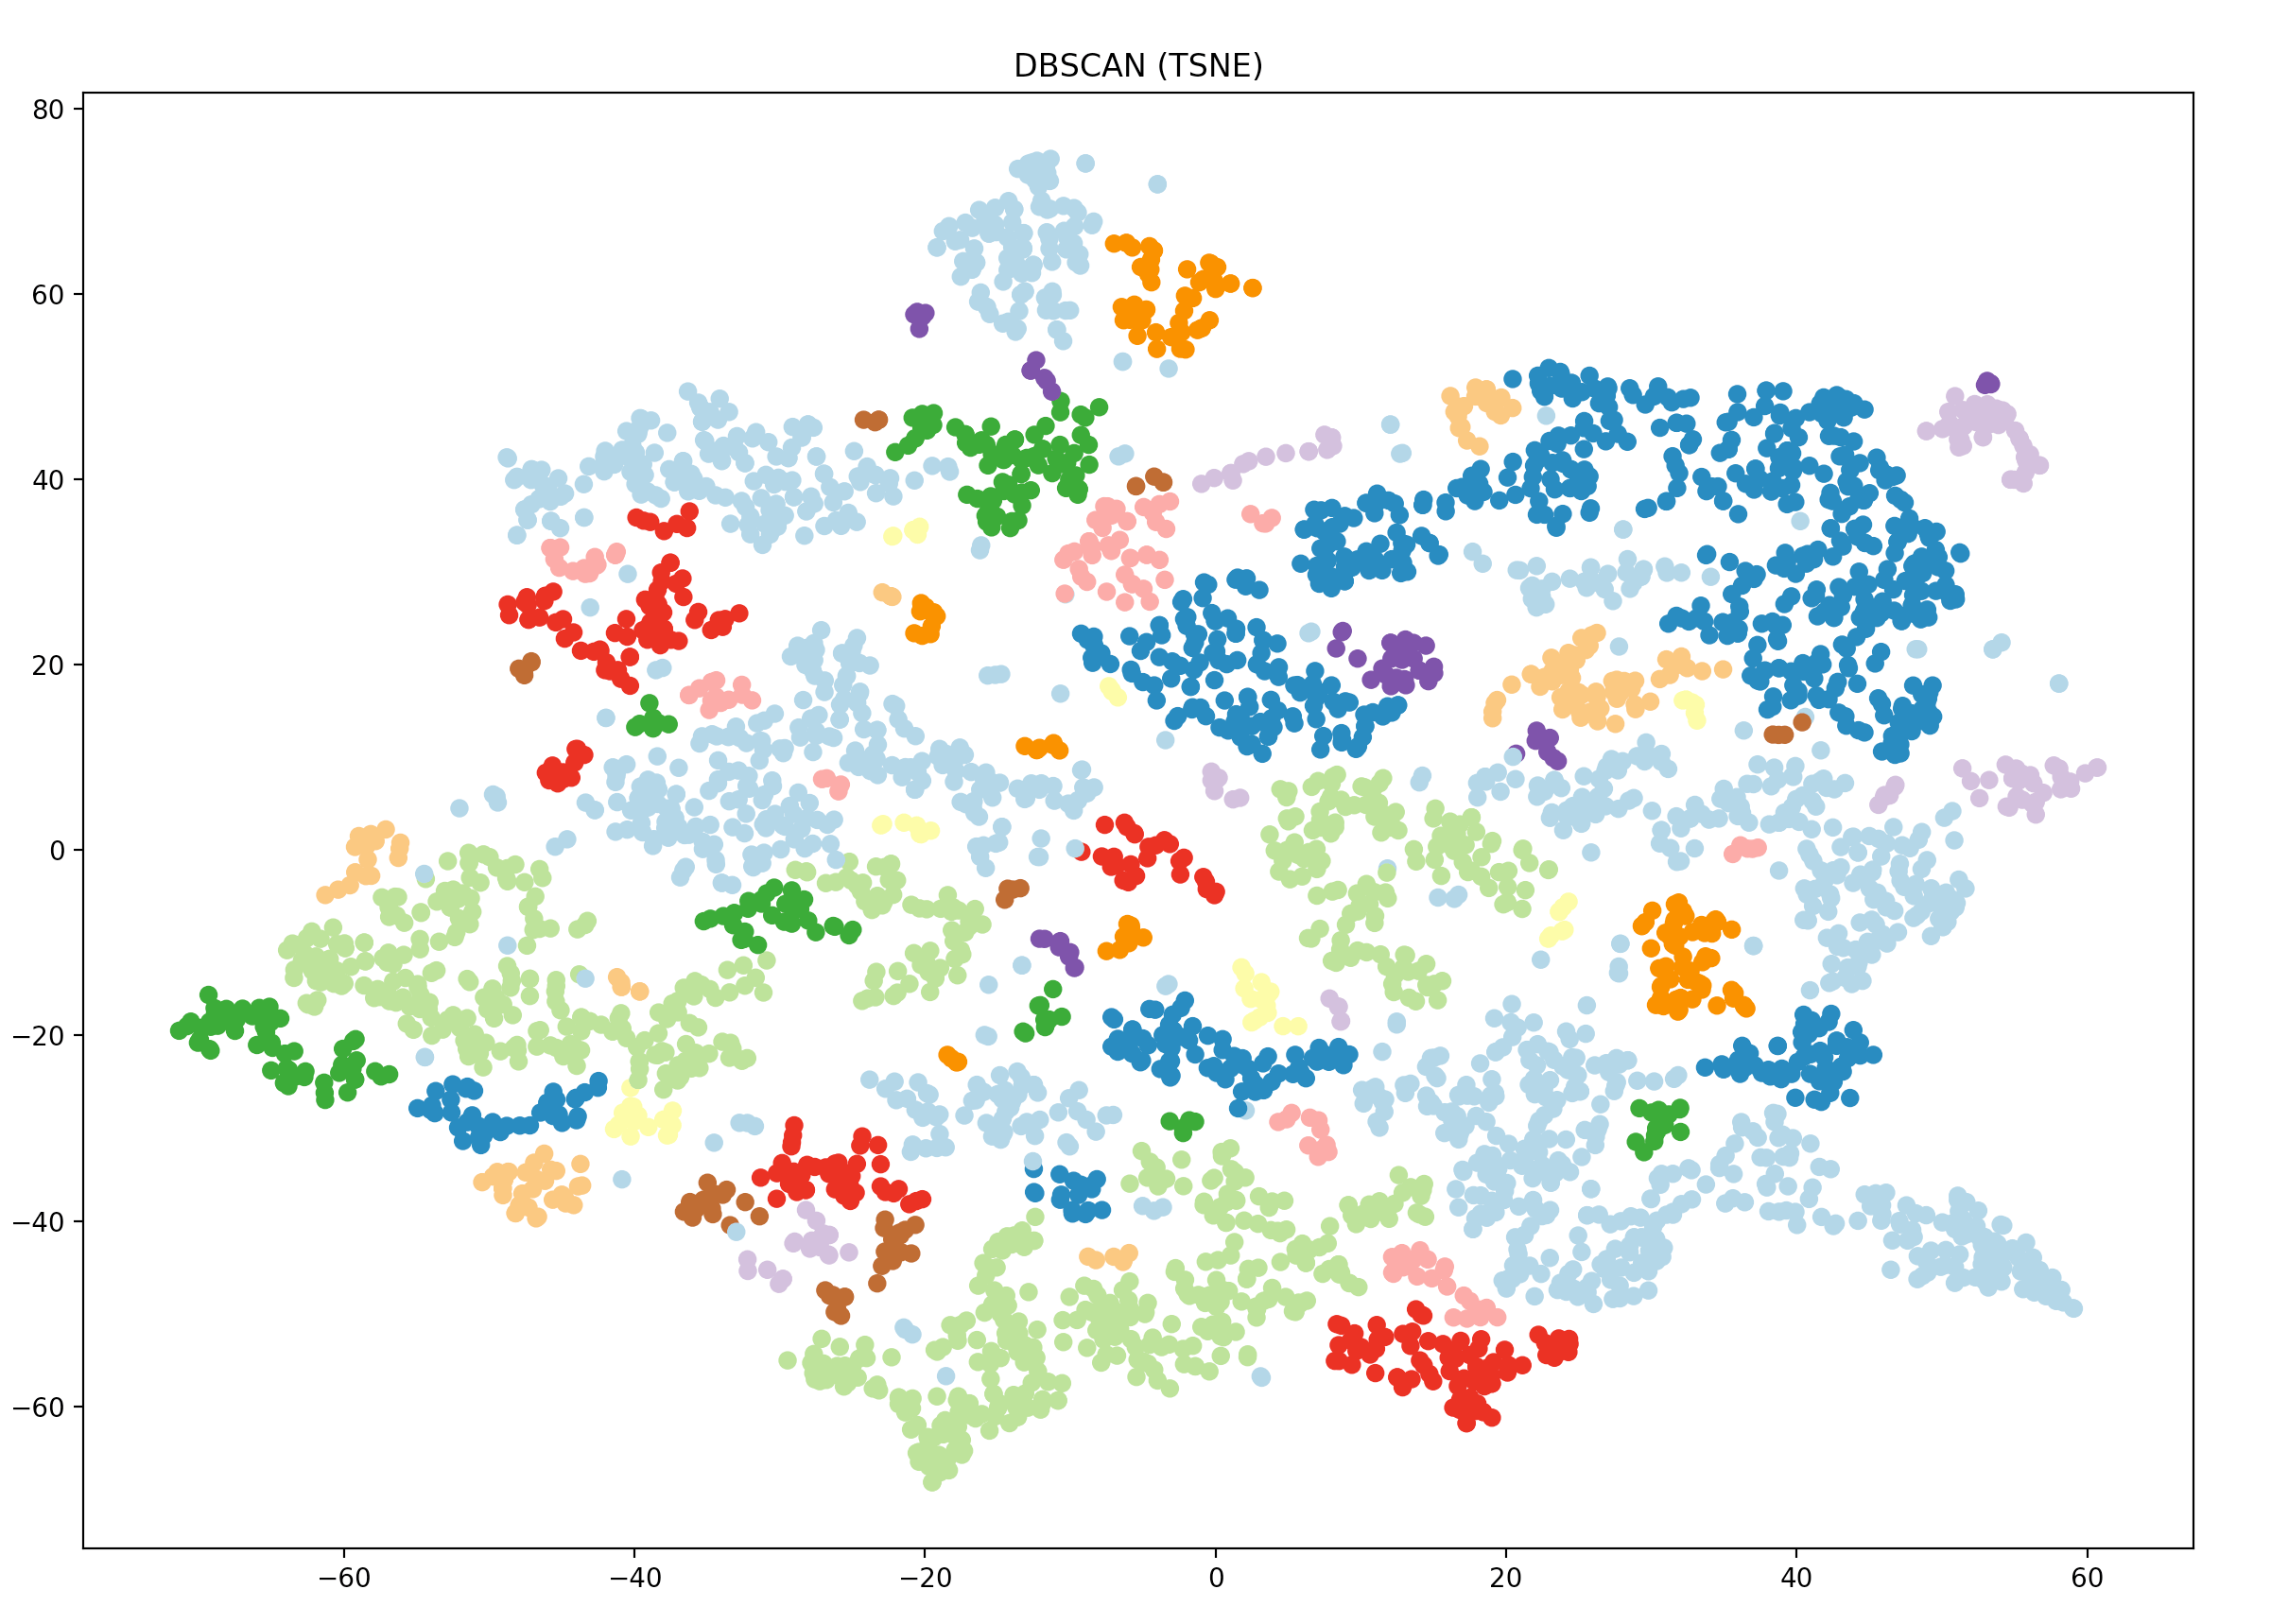
\includegraphics[width=0.9\textwidth]{./images/clusteringResults/3h-3-DBSCAN.png}
  \end{subfigure}%
  \begin{subfigure}{.5\textwidth}
    \centering
    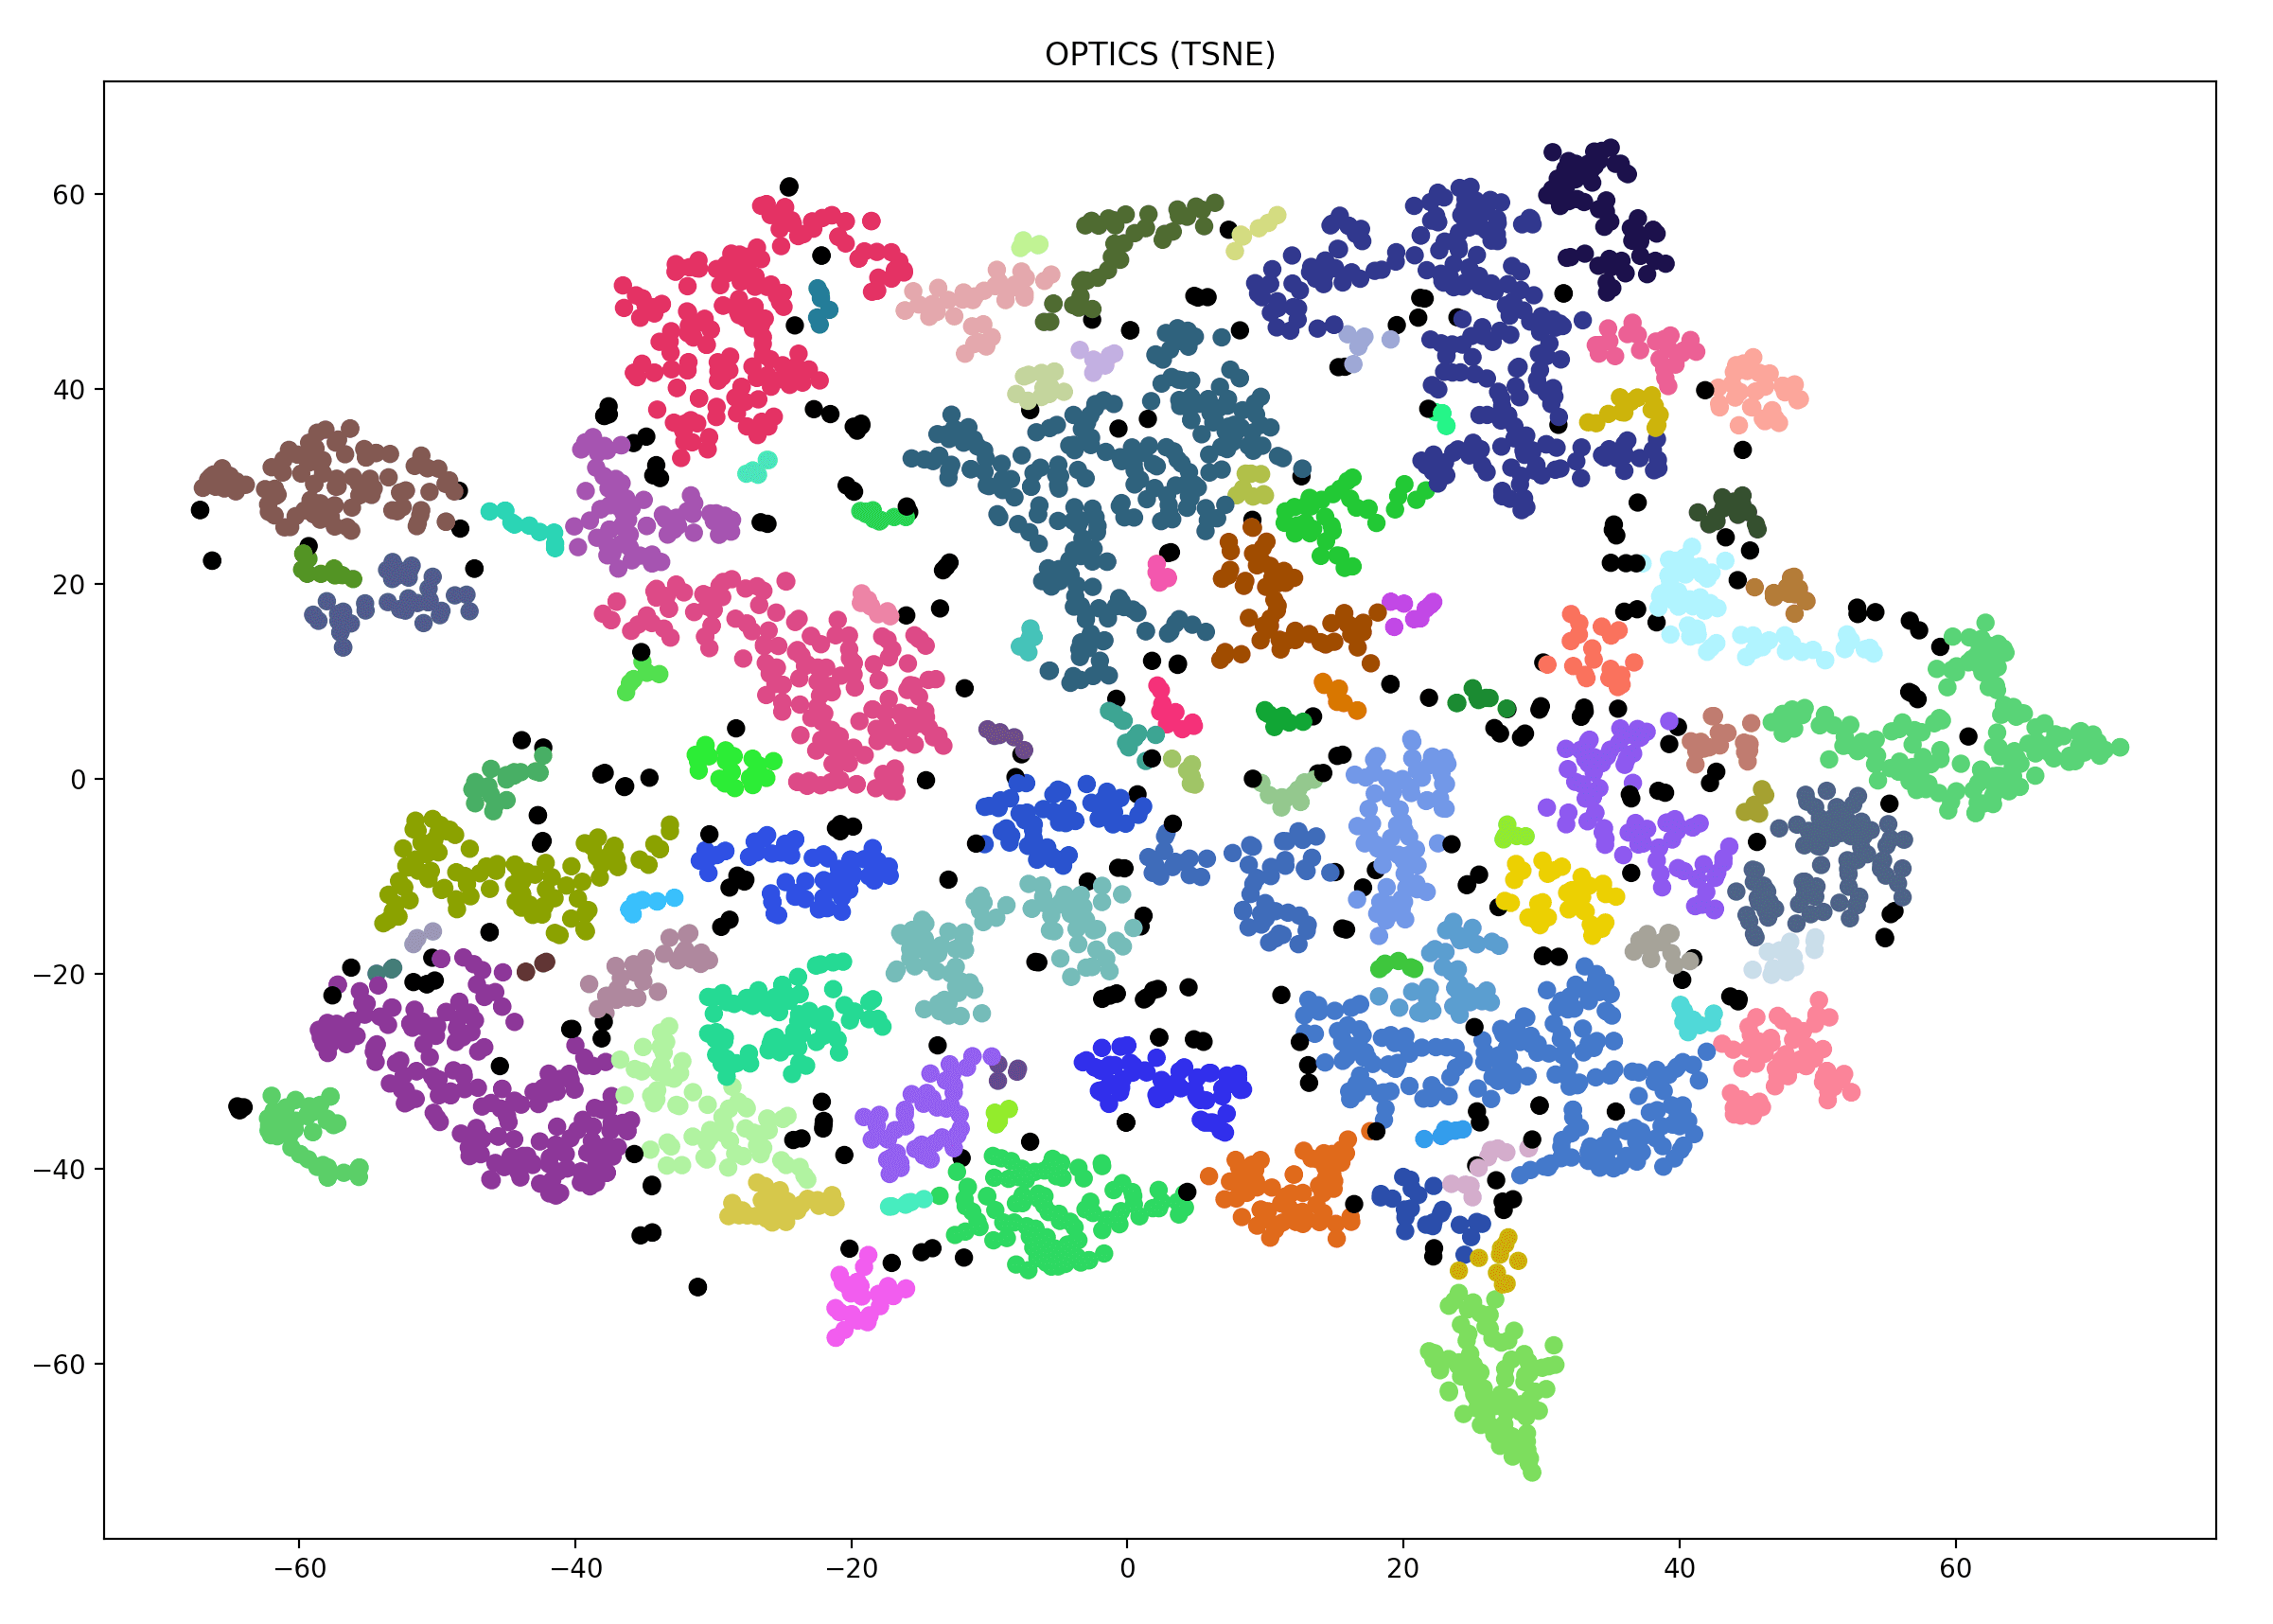
\includegraphics[width=0.9\textwidth]{./images/clusteringResults/3h-3-OPTICS.png}
	\end{subfigure}
	\caption{Comparison of the scatter plots from the DBSCAN (a) and OPTICS (b) clusterings of the average of the 1st column to the 3rd column, so the first \textbf{1.5 hours} (3h data files: 30 minutes, 1 hour \& 1 hour 30 minutes).}
  \label{figure:finalClustering3h-3}
\end{figure}

\begin{figure}[H]
	\centering
	\begin{subfigure}{.5\textwidth}
    \centering
    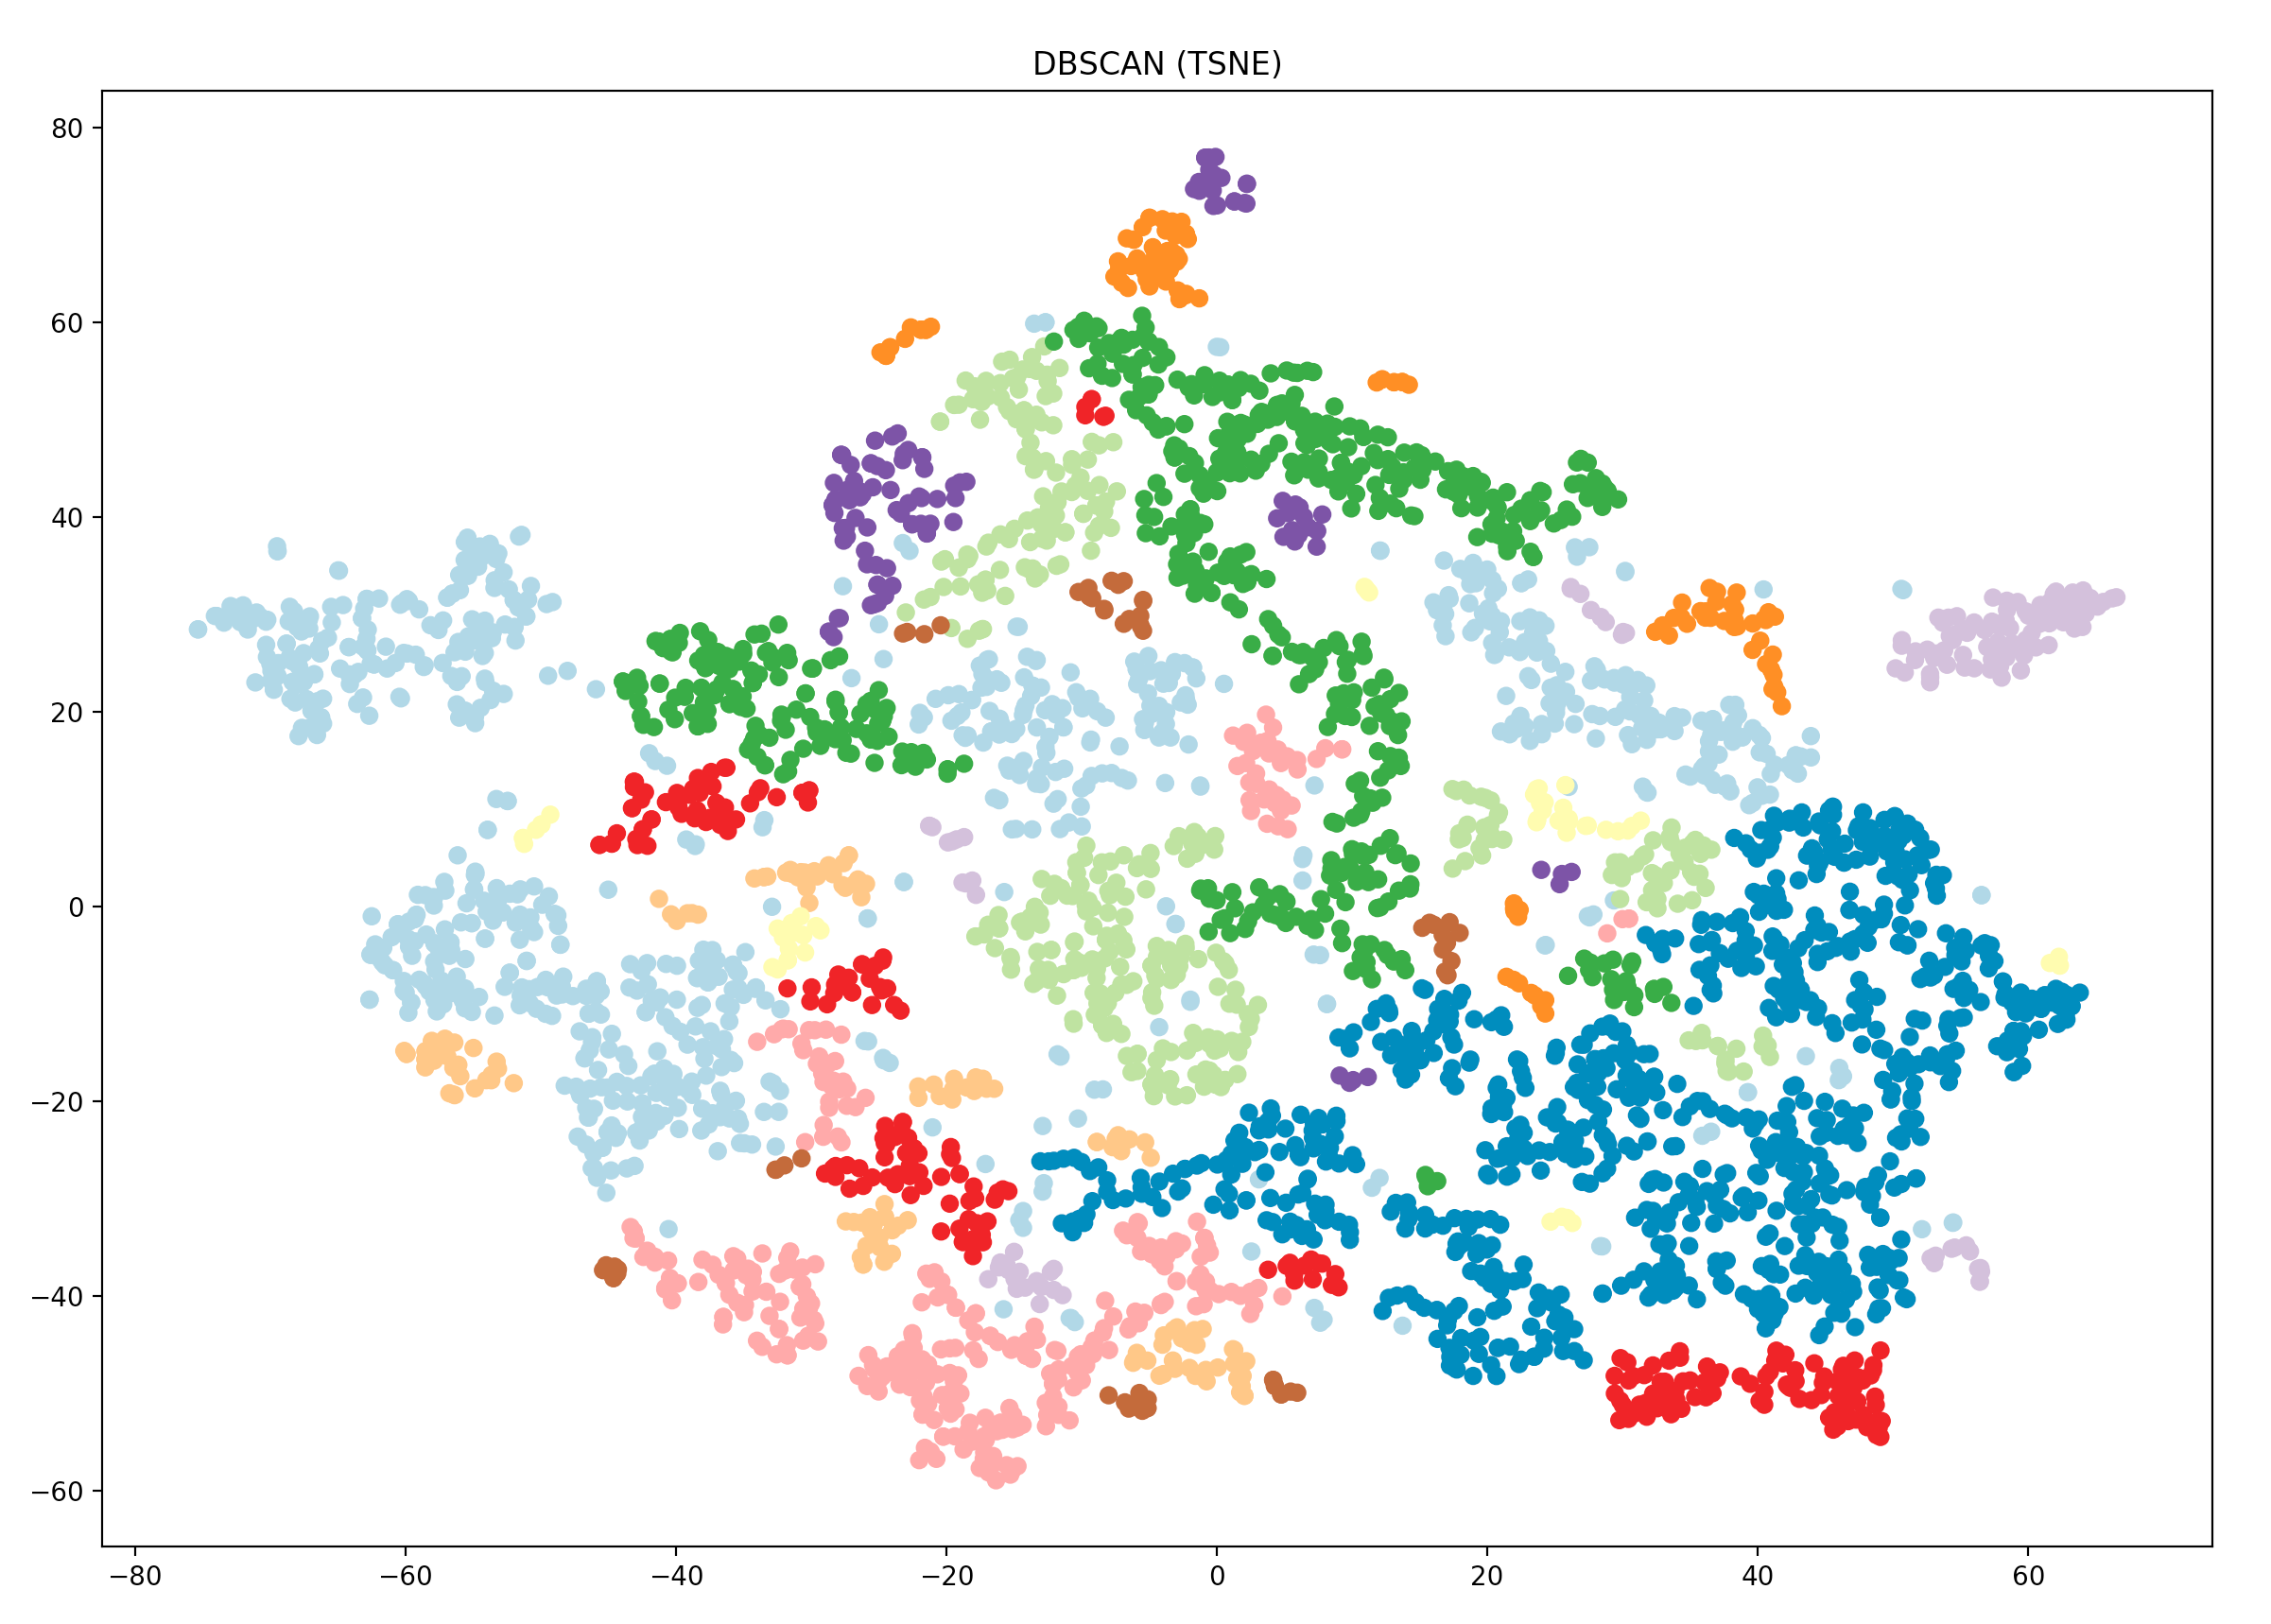
\includegraphics[width=0.9\textwidth]{./images/clusteringResults/3h-4-DBSCAN.png}
  \end{subfigure}%
  \begin{subfigure}{.5\textwidth}
    \centering
    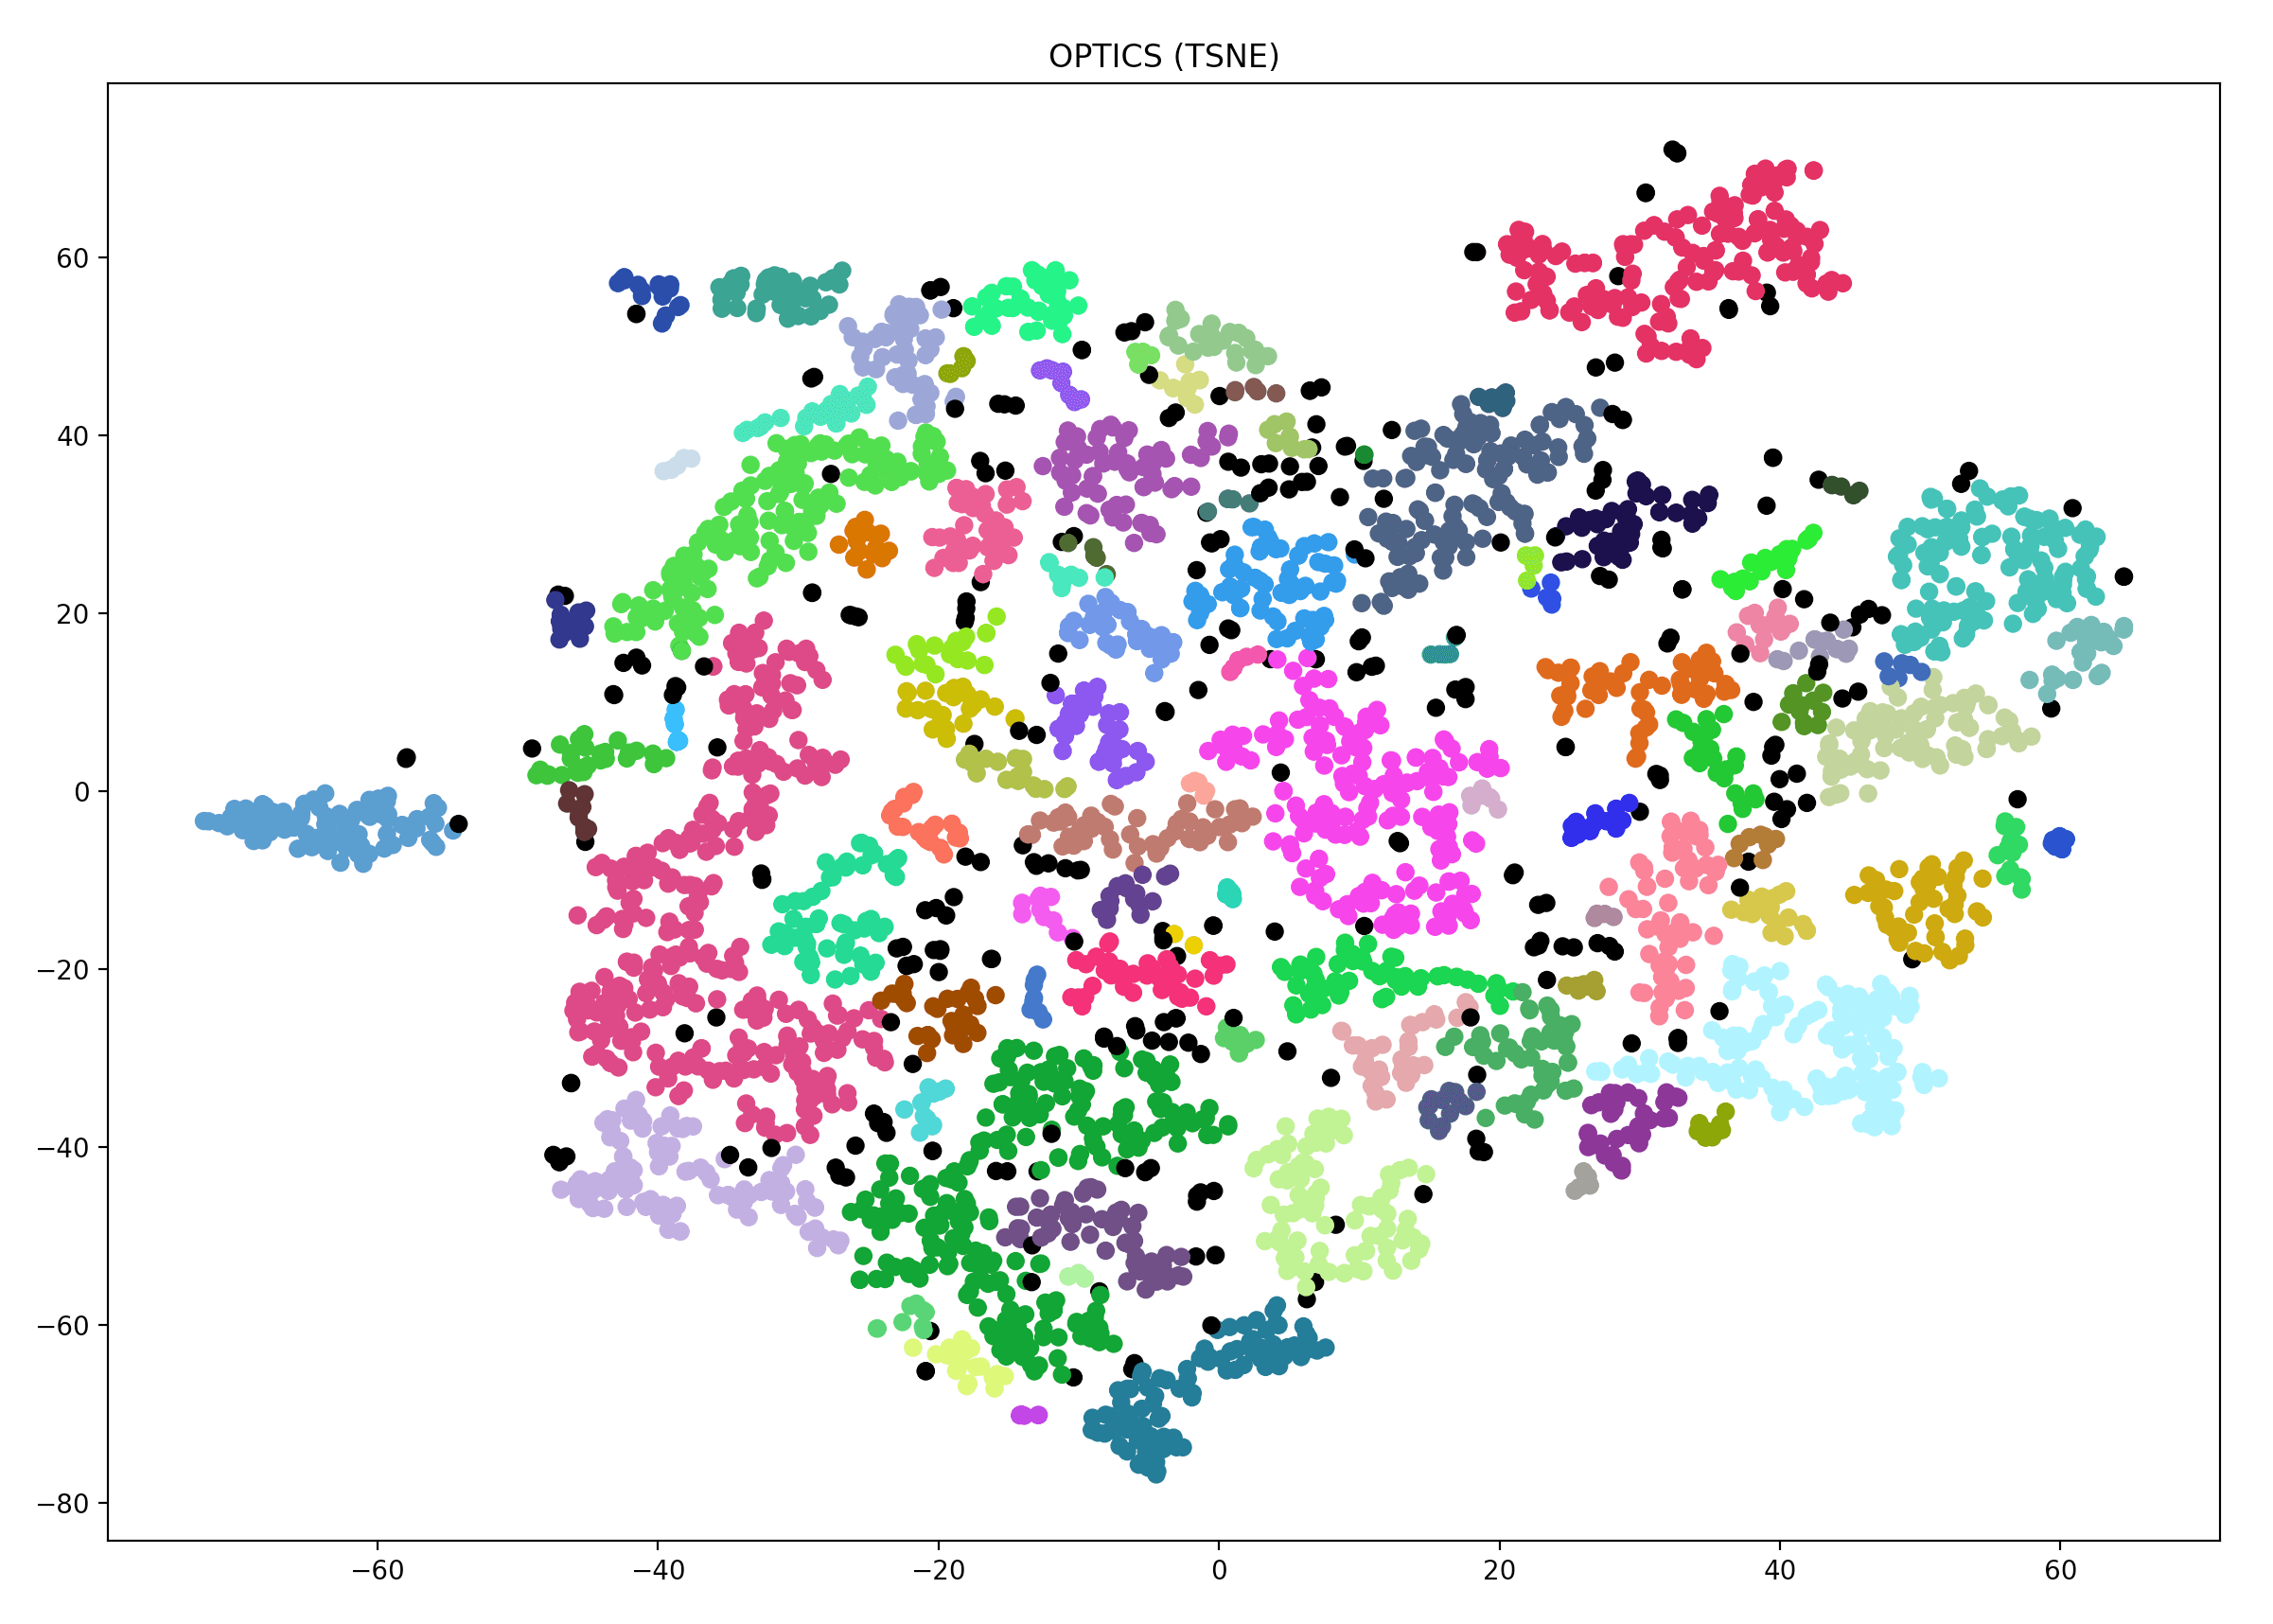
\includegraphics[width=0.9\textwidth]{./images/clusteringResults/3h-4-OPTICS.png}
	\end{subfigure}
	\caption{Comparison of the scatter plots from the DBSCAN (a) and OPTICS (b) clusterings of the average of the 1st column to the 4th column, so the first \textbf{2 hours} (3h data files: 30 minutes, 1 hour, 1 hour 30 minutes \& 2 hours).}
  \label{figure:finalClustering3h-4}
\end{figure}


\begin{figure}[H]
	\centering
	\begin{subfigure}{.5\textwidth}
    \centering
    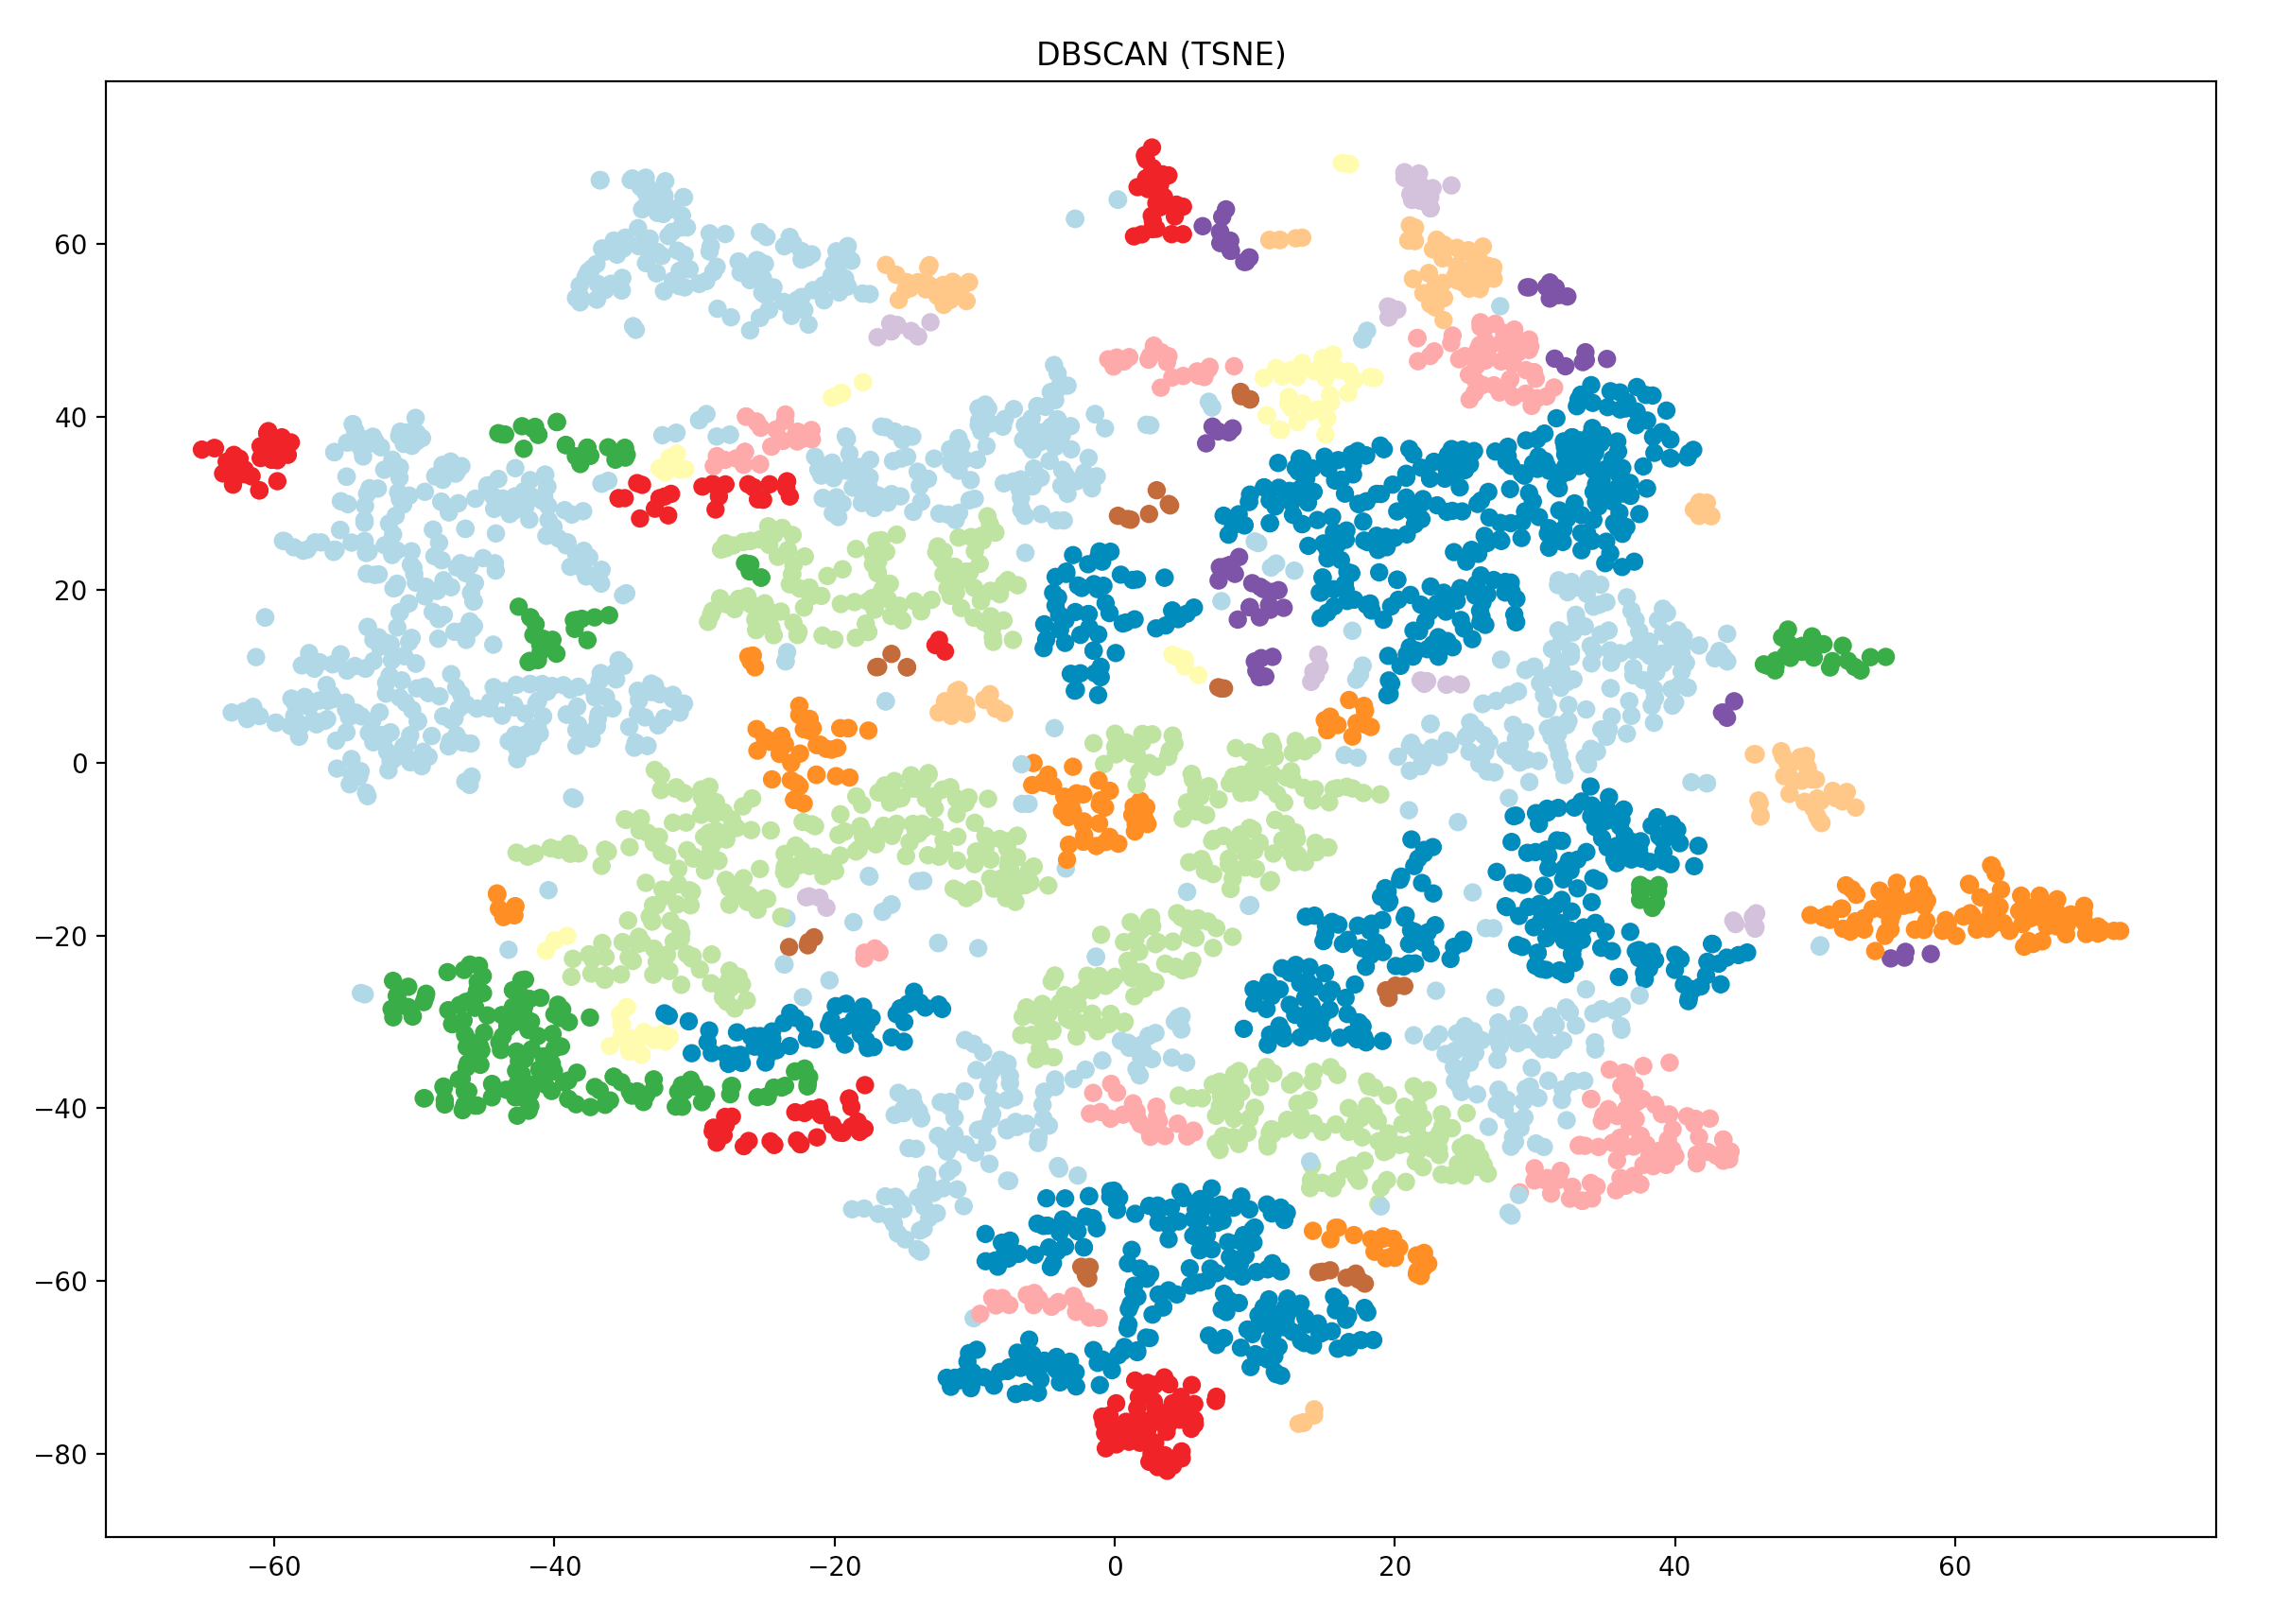
\includegraphics[width=0.9\textwidth]{./images/clusteringResults/3h-5-DBSCAN.png}
  \end{subfigure}%
  \begin{subfigure}{.5\textwidth}
    \centering
    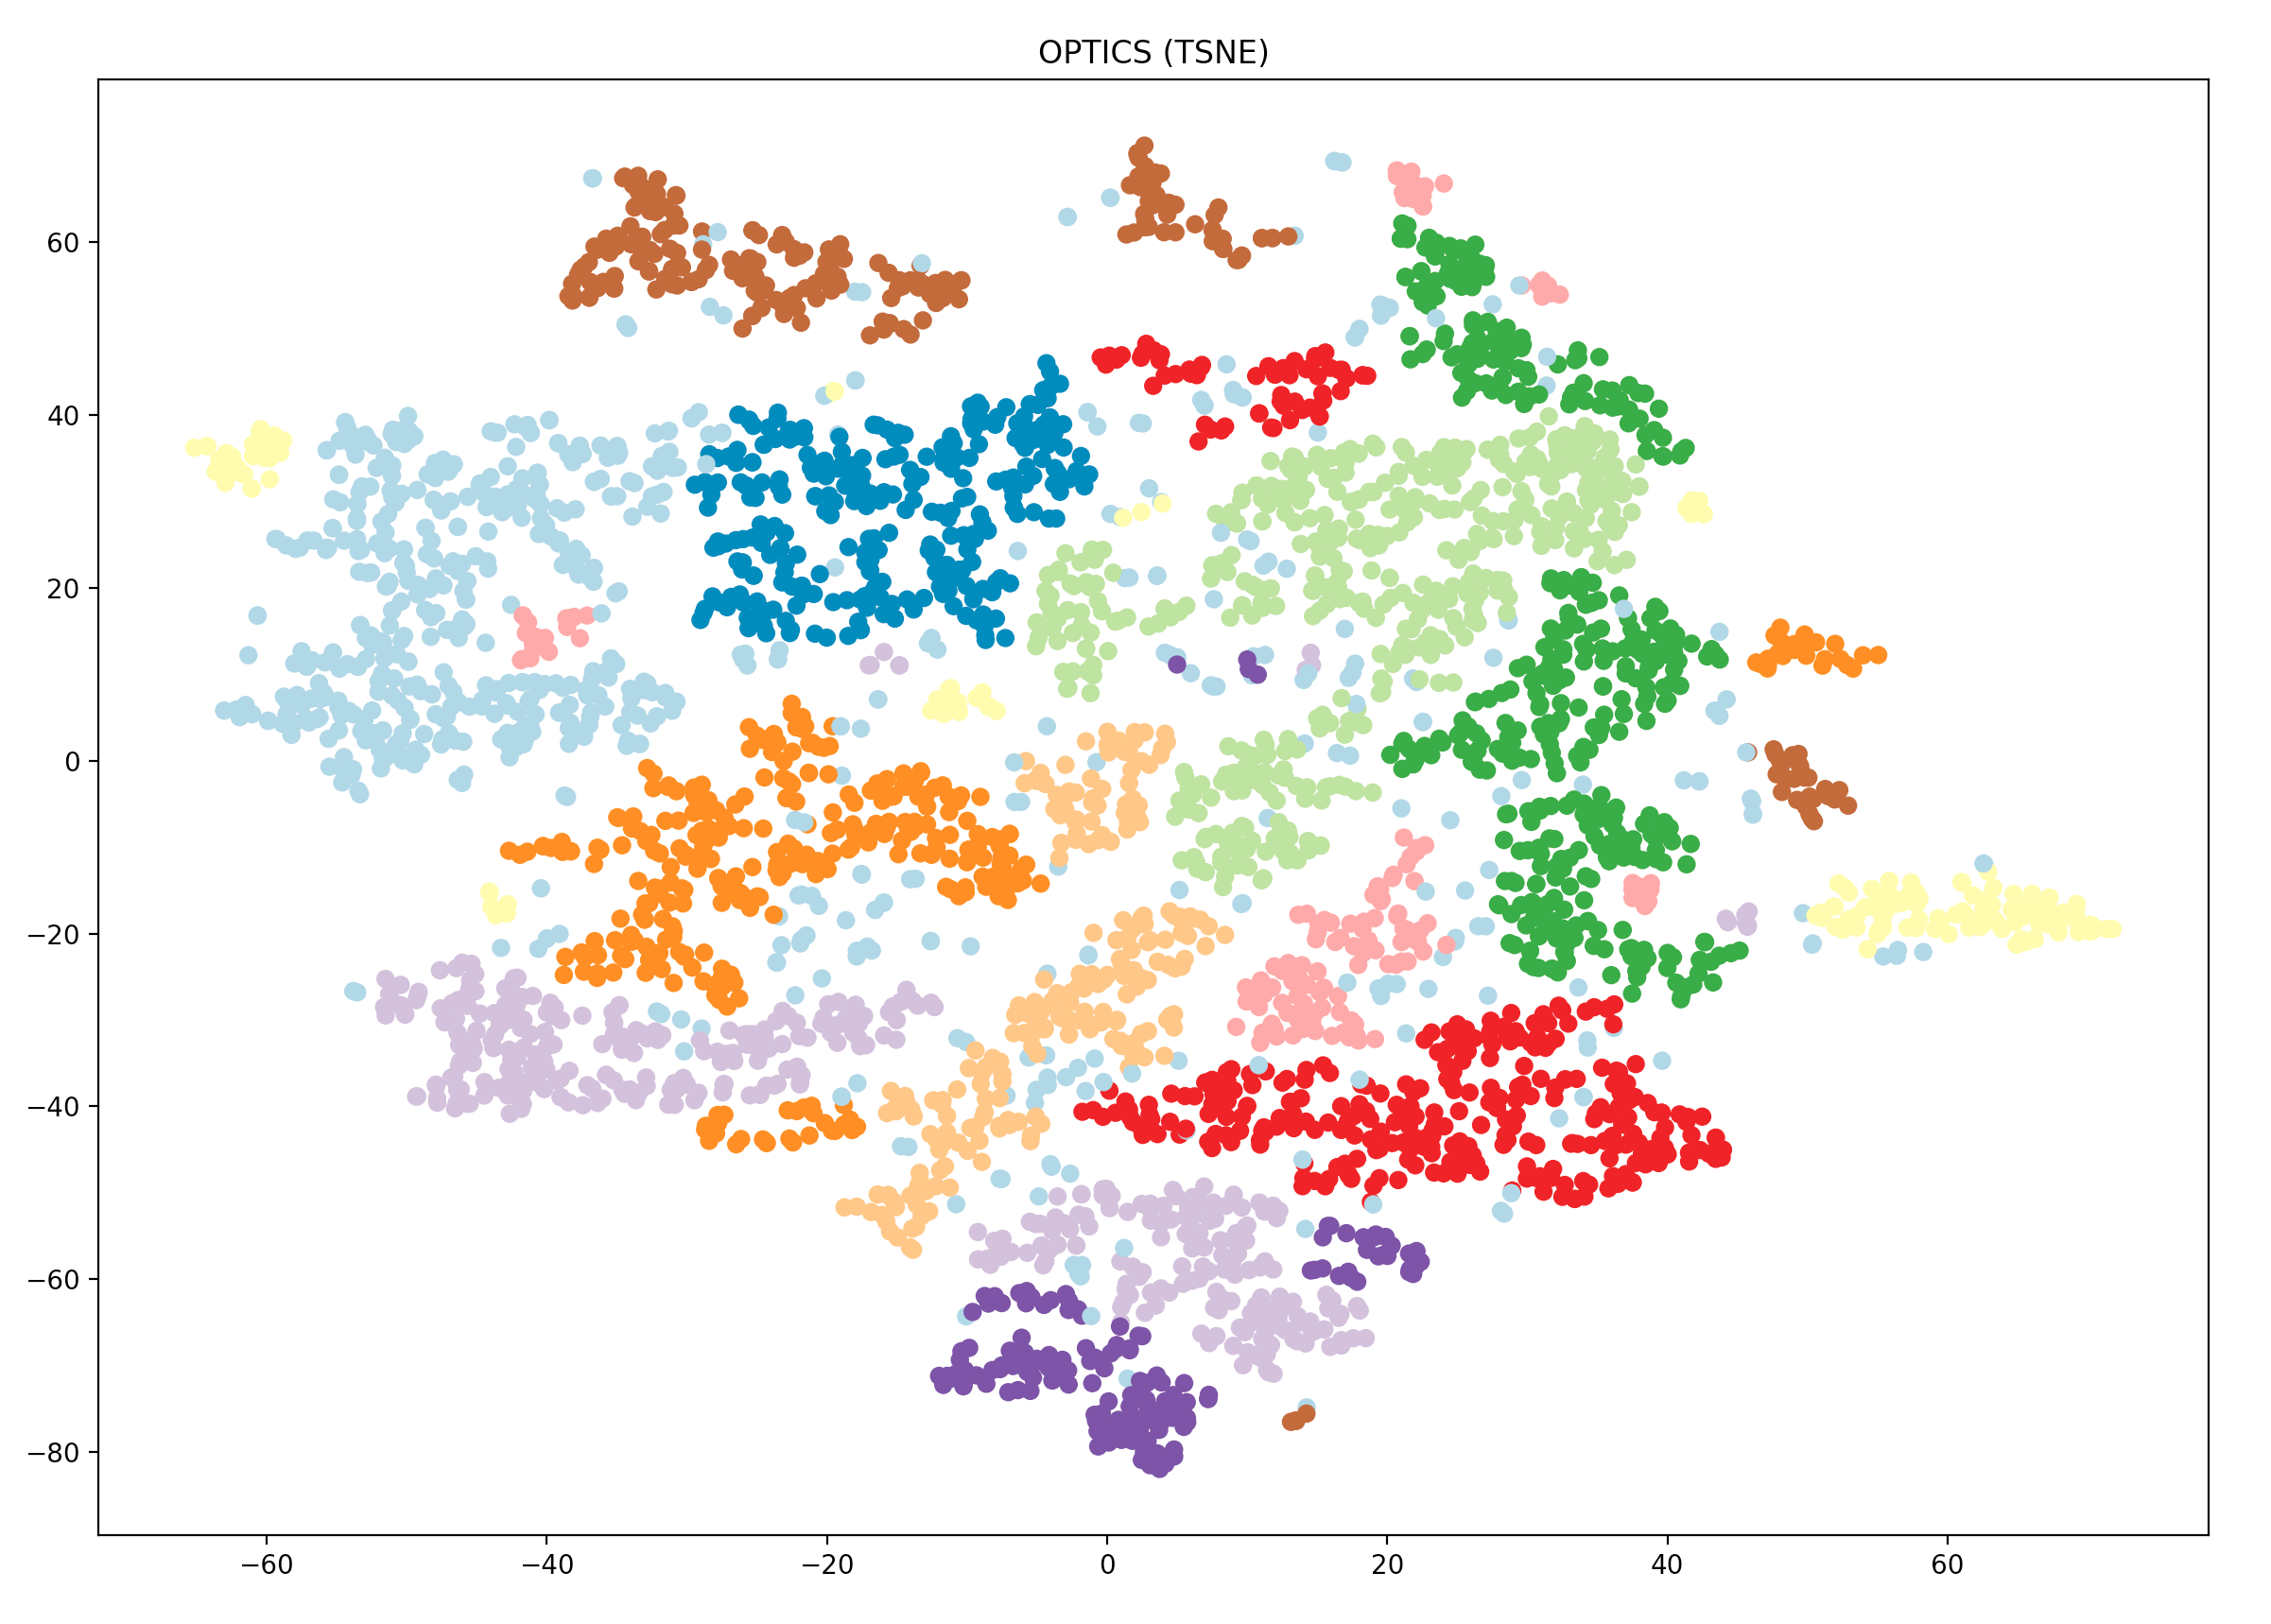
\includegraphics[width=0.9\textwidth]{./images/clusteringResults/3h-5-OPTICS.png}
	\end{subfigure}
	\caption{Comparison of the scatter plots from the DBSCAN (a) and OPTICS (b) clusterings of the average of the 1st column to the 5th column, so the first \textbf{2.5 hours} (3h data files: 30 minutes, 1 hour, 1 hour 30 minutes, 2 hours \& 2 hours 30 minutes).}
  \label{figure:finalClustering3h-5}
\end{figure}


\begin{figure}[H]
	\centering
	\begin{subfigure}{.5\textwidth}
    \centering
    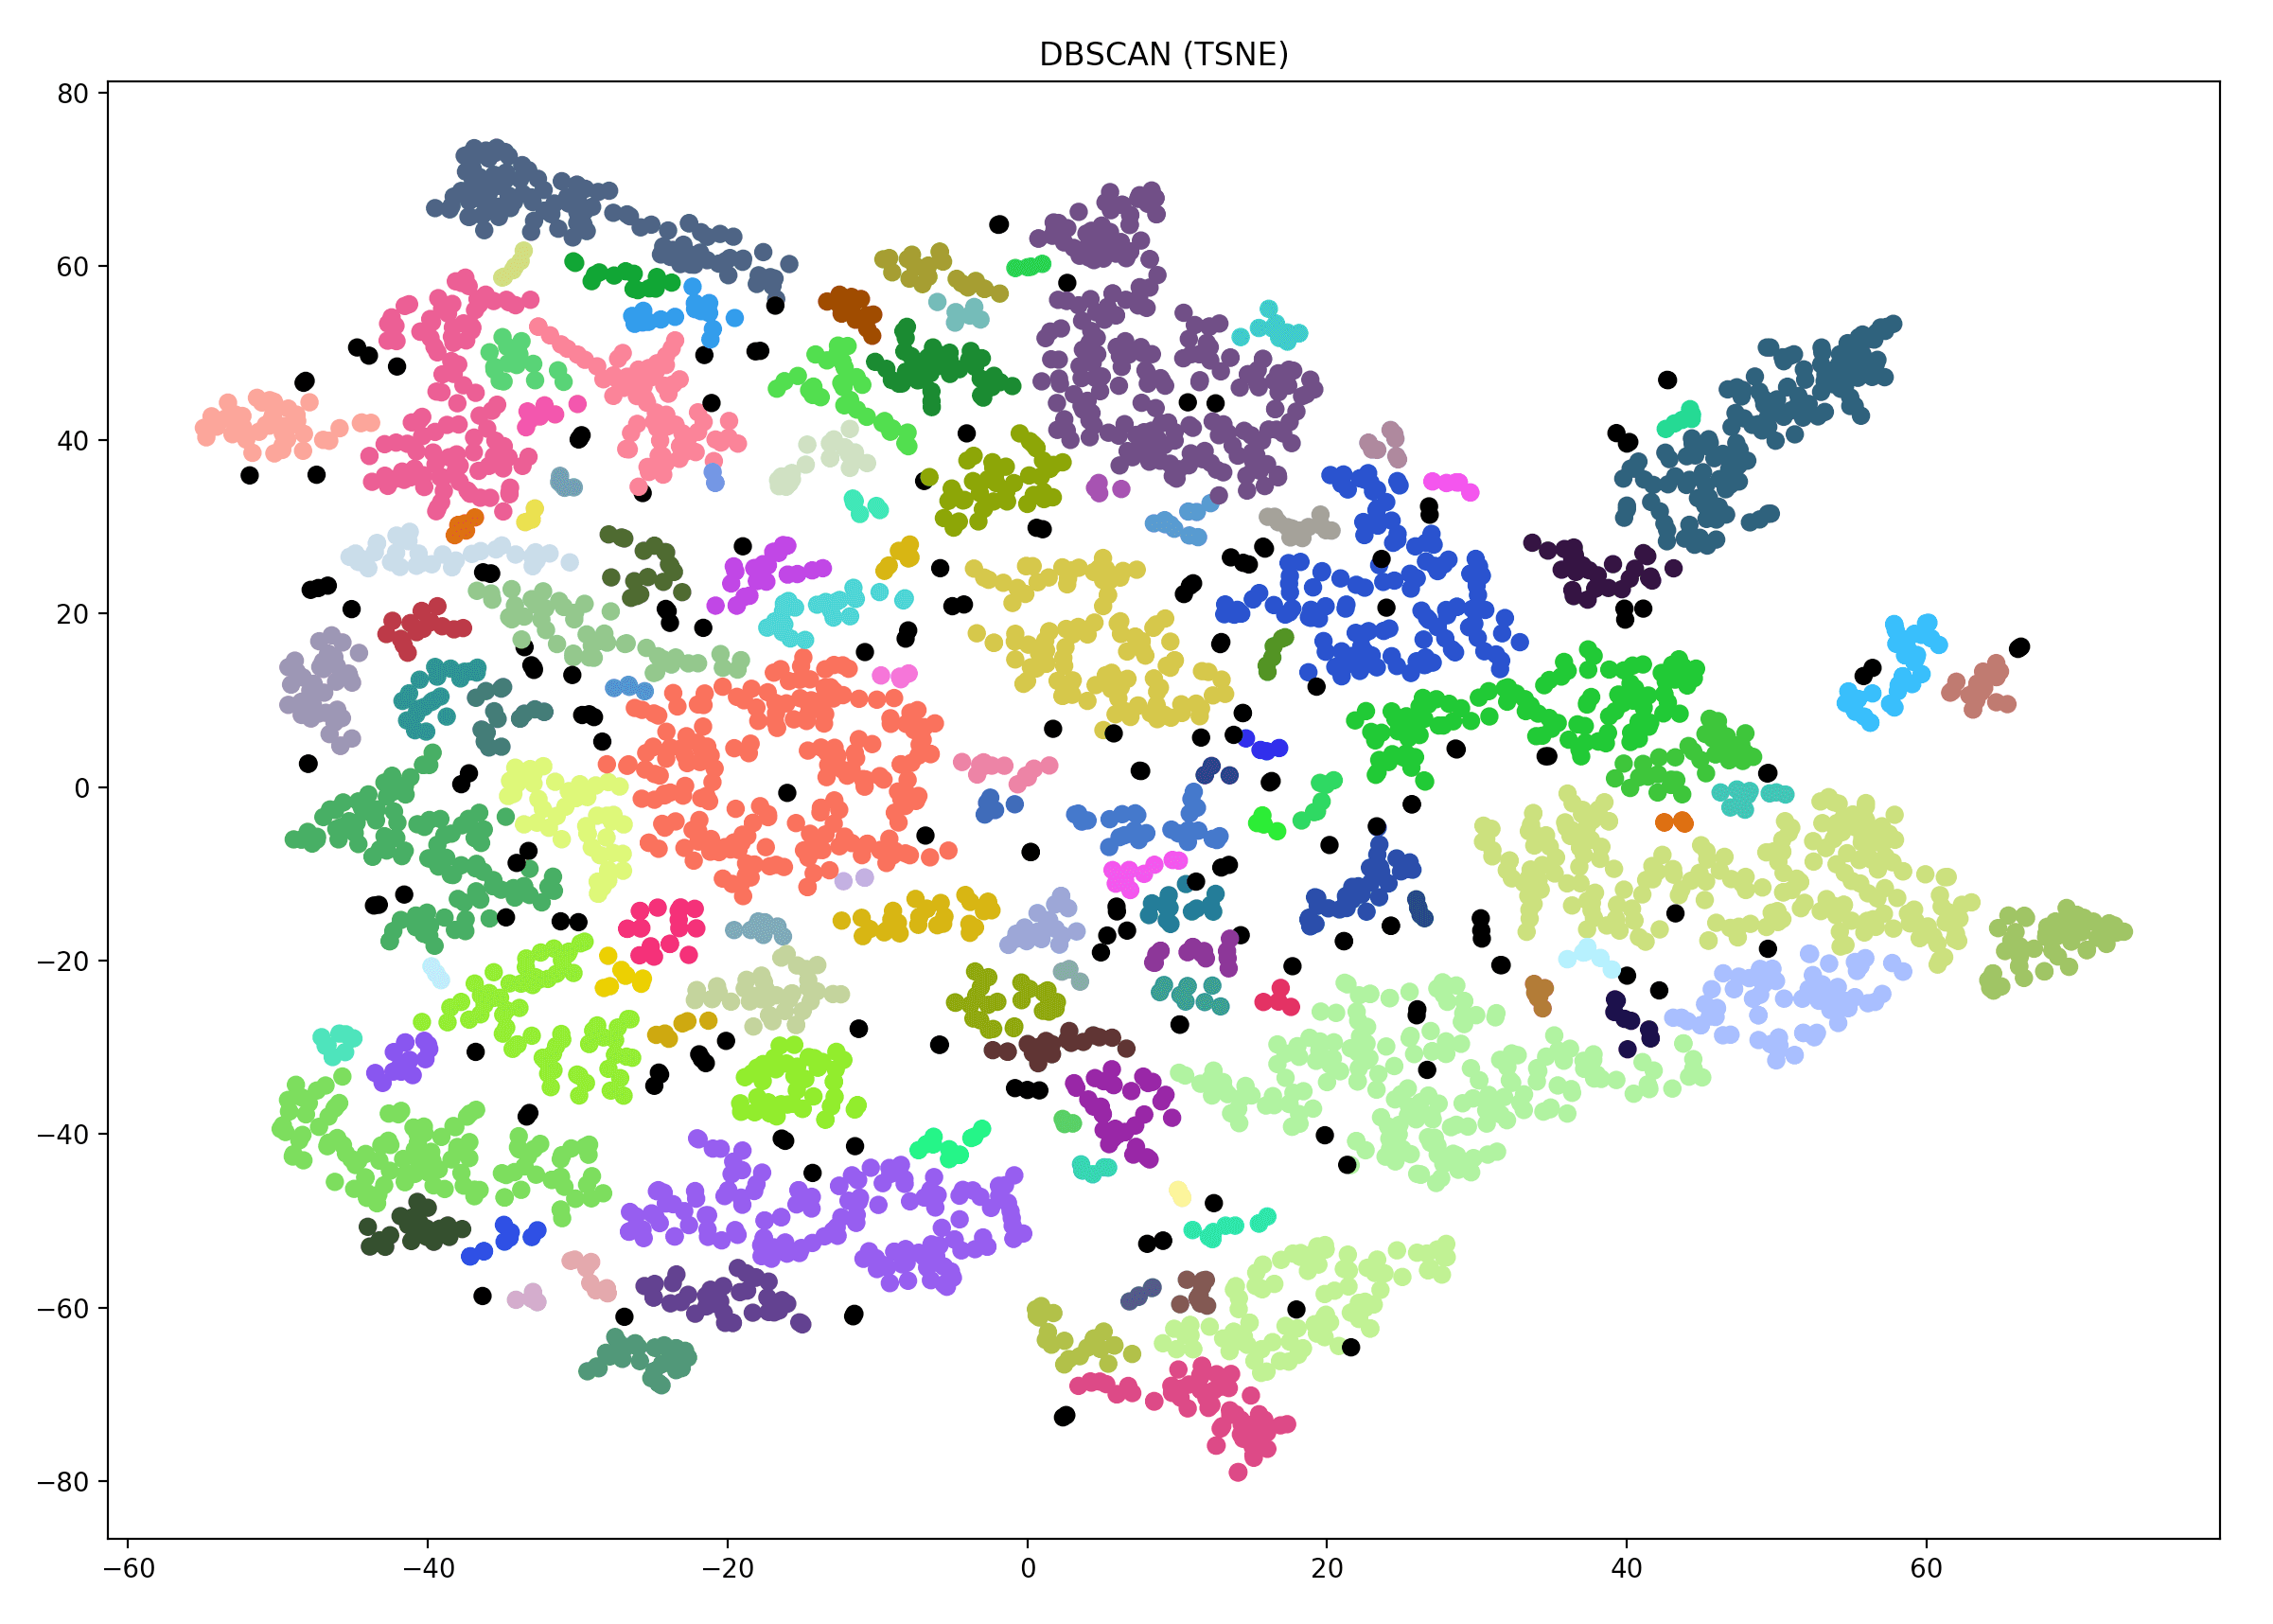
\includegraphics[width=0.9\textwidth]{./images/clusteringResults/3h-6-DBSCAN.png}
  \end{subfigure}%
  \begin{subfigure}{.5\textwidth}
    \centering
    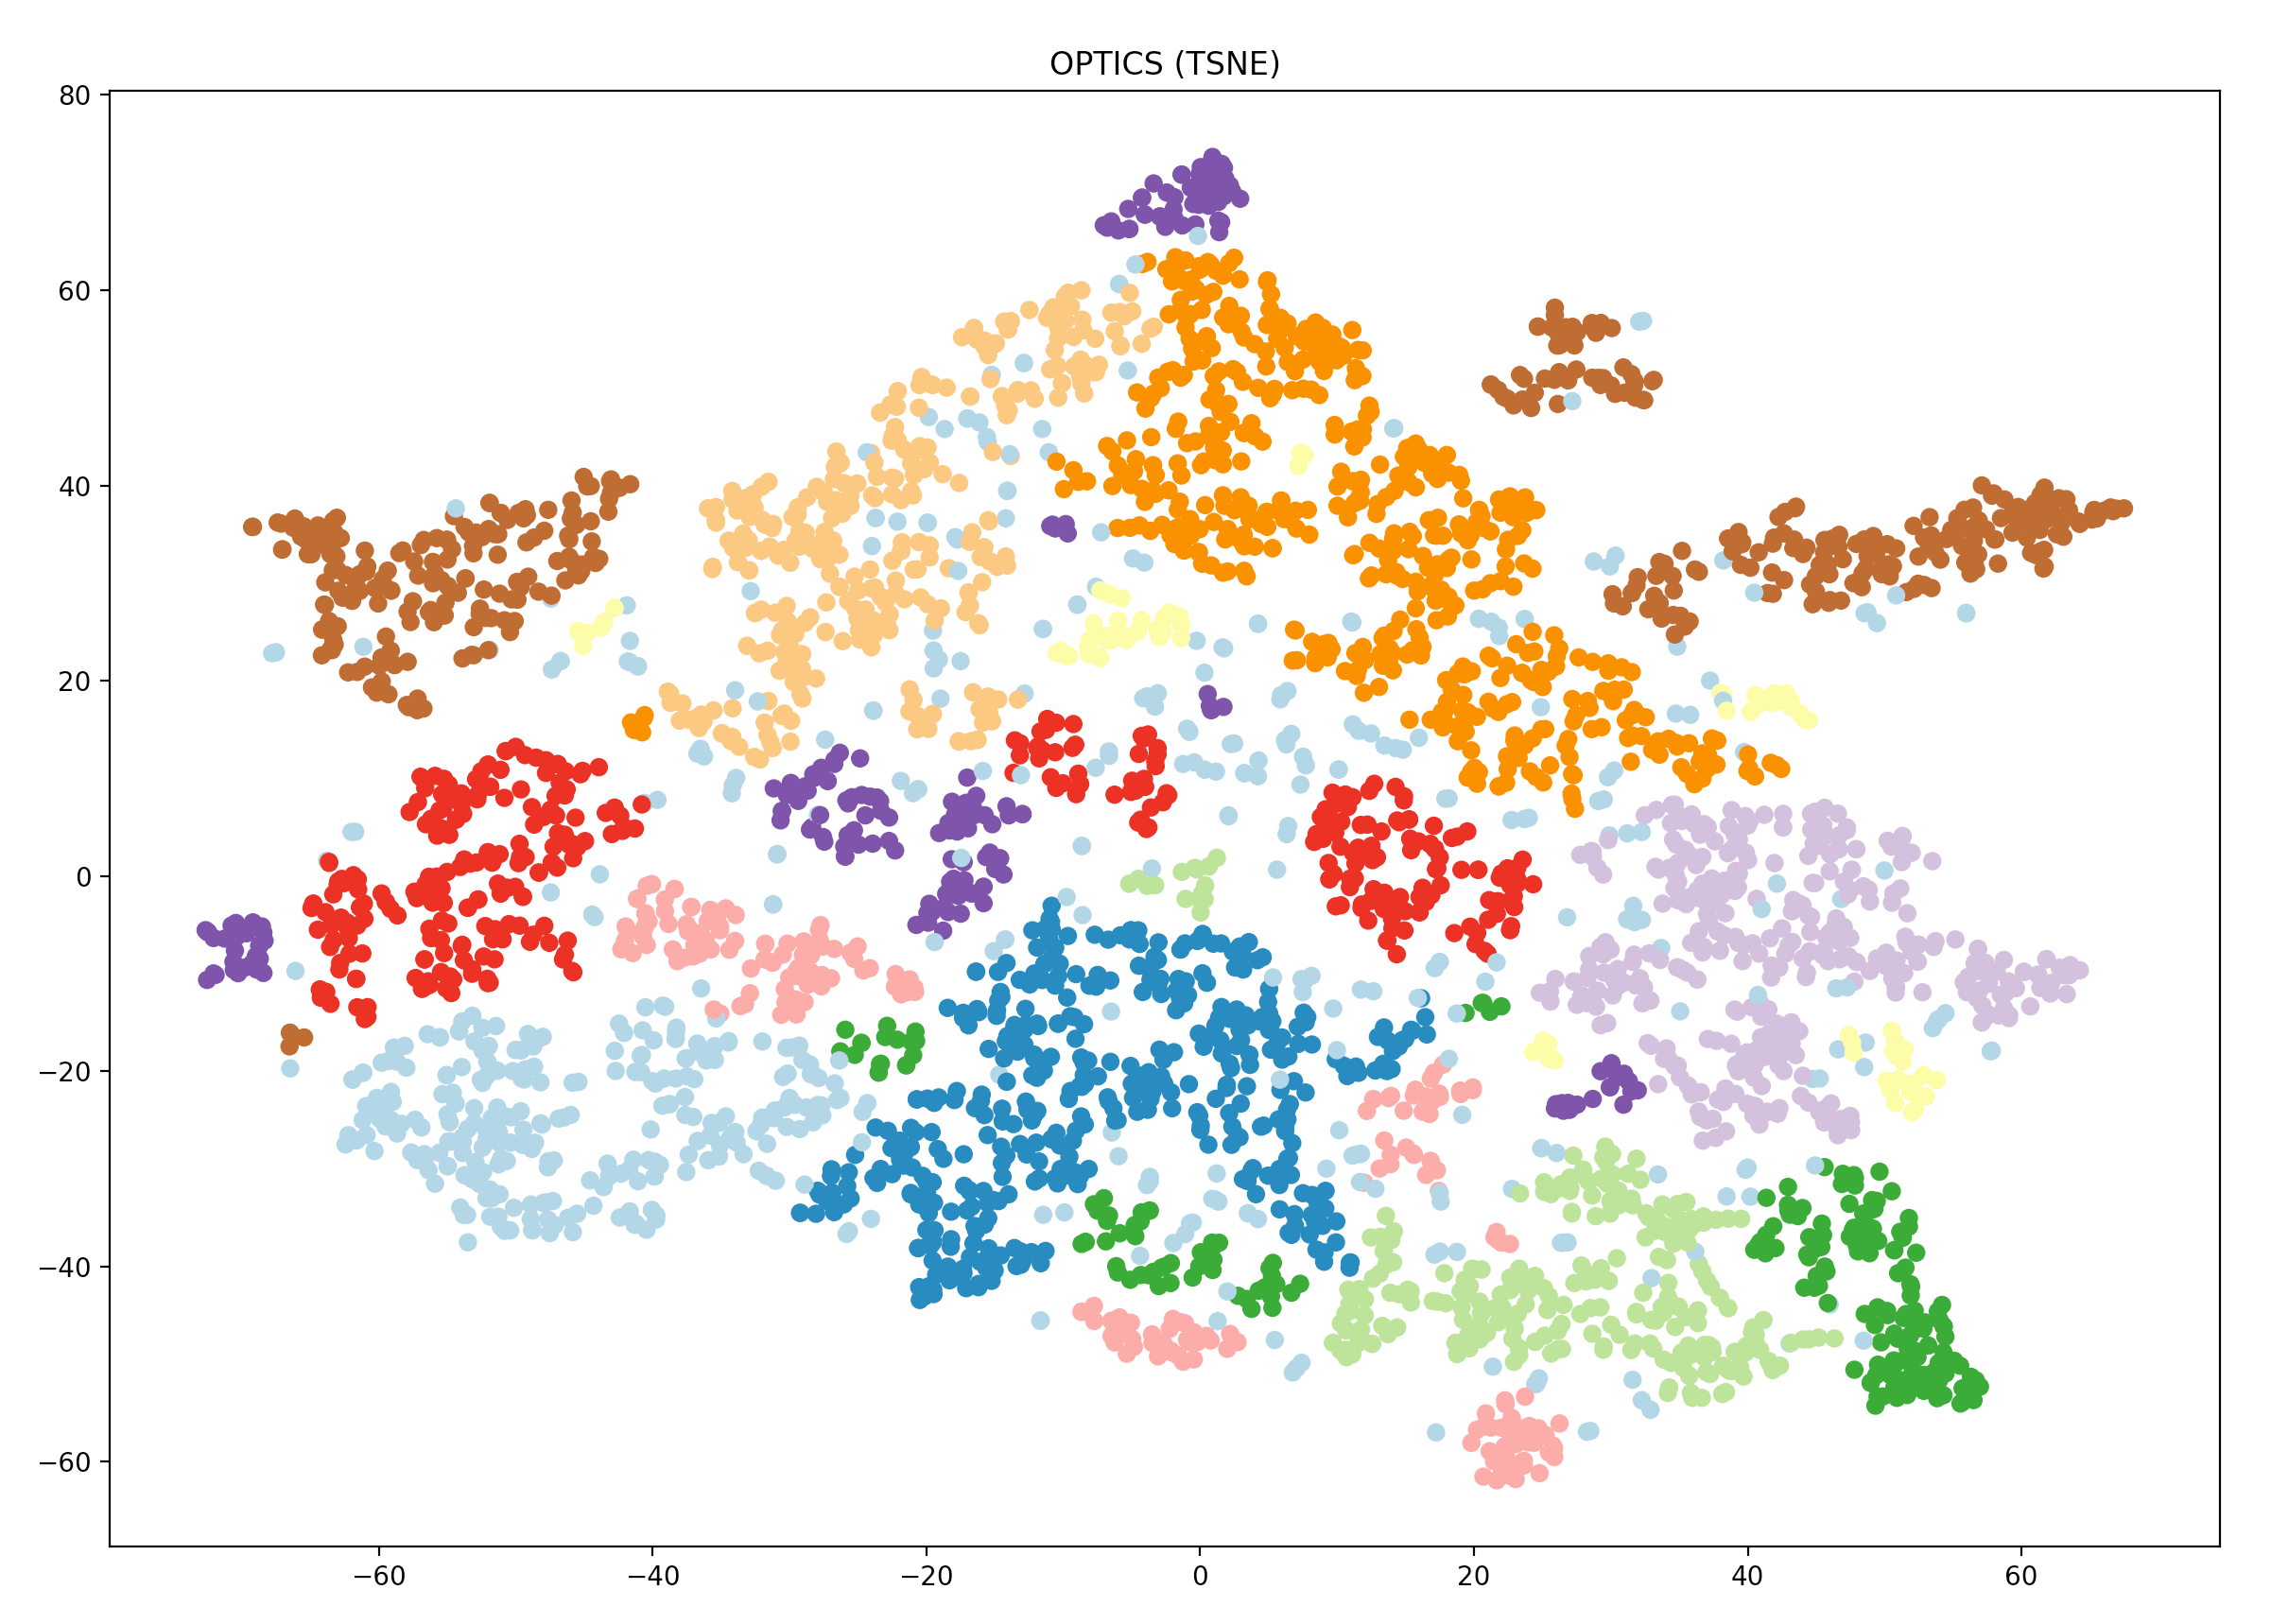
\includegraphics[width=0.9\textwidth]{./images/clusteringResults/3h-6-OPTICS.png}
	\end{subfigure}
	\caption{Comparison of the scatter plots from the DBSCAN (a) and OPTICS (b) clusterings of the average of the 1st column to the 6th column, so all \textbf{3 hours} (3h data files: 30 minutes, 1 hour, 1 hour 30 minutes, 2 hours, 2 hours 30 minutes \& 3 hours).}
  \label{figure:finalClustering3h-6}
\end{figure}


\clearpage

